\chapter{Difference Smooths}
\label{appendix:difference_smooths}

Difference smooths are one way to determine whether two predicted curves are significantly different from one another. In this case, they are done using the \texttt{get\_difference} function in the \texttt{itsadug} package. While \texttt{itsadug} provides a function to plot these difference smooths, for the purpose of this dissertation, I took the same data and produced custom plots to better highlight areas of significance. 

As their name implies, they are calculated as the difference (i.e. subtracting) one curve from the other. As a basic example, if two curves were identical, the difference smooth would be a flat line at zero. If two curves were identical in shape but with different positions vertically, their difference smooth would also be a flat line intersecting the \textit{y}-axis at the value representing the difference between those two curves. When two curves take different shapes, the difference smooth is still one subtracted by the other, but the resulting shape will look somewhat different than either of the two original curves.

For example, a GAM was fit to the following artificual, arbitrary data (from chapter \ref{ch:methodology}), resulting in a smooth for the blue dots and a smooth for the red dots:

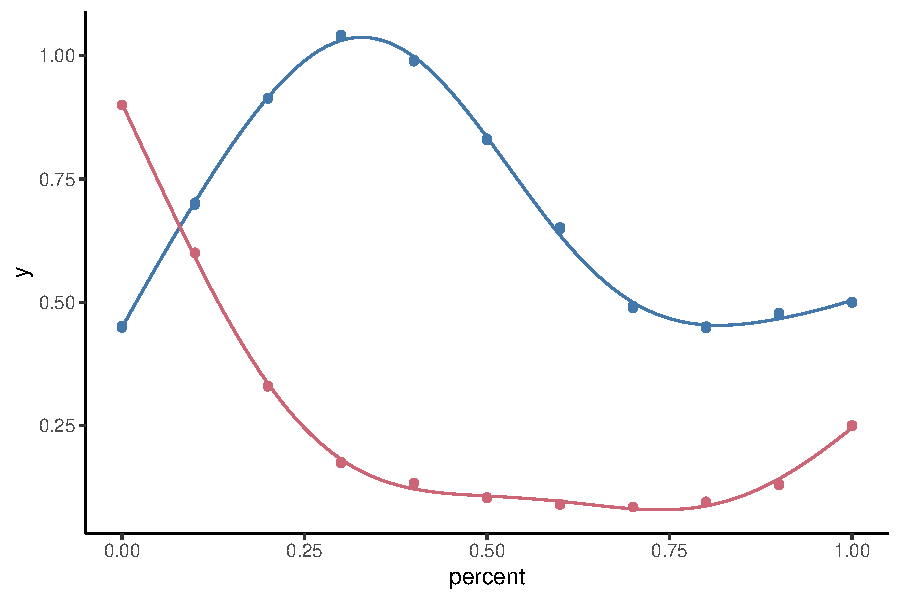
\includegraphics[width = 3in]{Figures/example_plots/sample_diff_smooth_data.pdf}

\noindent
When comparing the blue curve to the red curve, the difference smooth looks like this.

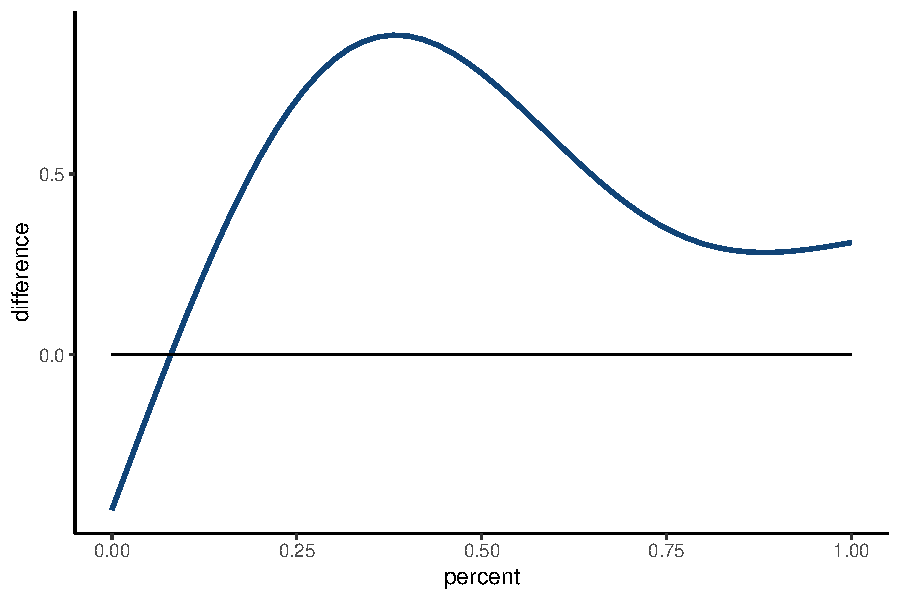
\includegraphics[width = 3in]{Figures/example_plots/sample_diff_smooth.pdf}

\noindent
Here, the blue curve is the reference value, so this smooth represents the blue curve minus the red smooth. For example, looking at the onset in the original data, since the blue curve is lower than the red in the original data, the difference is negative. At 40\% into the duration of the vowel, the blue curve is near its maximum while red is quite low, so the difference smooth is also quite high. As the difference between the two curves gets smaller towards the offset, the difference smooth gets closer to zero.

In addition to the difference smooths themselves, \texttt{get\_difference} also returns 95\% confidence intervals around the smooths. Given a particular time point, the confidence interval includes zero, the difference between the two smooths at that timepoint is not statistically significant. In the sample data, the confidence intervals suggest that the difference between the blue and the red curves is only significant between approximately 20\% and 60\% into the duration of the vowel:

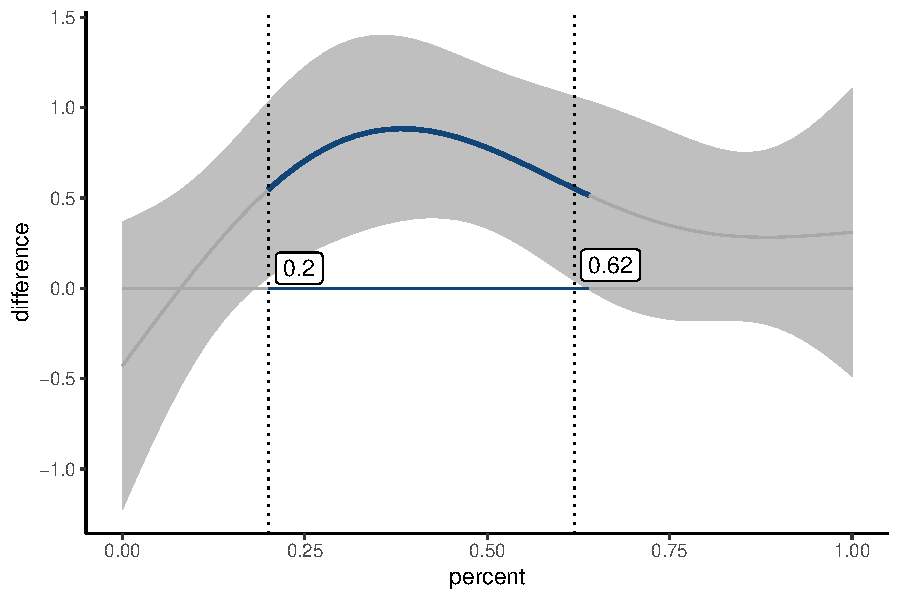
\includegraphics[width = 3in]{Figures/example_plots/sample_diff_smooth_sig.pdf}

Exactly two levels of a factor can be compared using difference smooths. That means that I cannot use them to see if men are different from women generally, but rather, I can see if the F1 of \bat for Millennial women is different from the F1 of \bat for Gen X women. Therefore, for any vowel, there are numerous difference smooths that can be calculated given the models used in this study.

This appendix shows select difference smooths for each vowel. Obviously there is no need to compare F1 to F2 for any vowel, so those are not displayed. Difference smooths that compare generations are presented first as the larger grid of panels. Difference smooths that compare between the sexes are displayed as a separate, smaller grid of plots.

In the generation panels (the larger grid), the plots are organized in columns by sex and by formant. The left half of the panels are the women (in shades of red) and the right half are the men (in shades of blue). Within the sexes, the left columns (i.e. columns 1 and 3) are for F1 and the right columns (i.e. columns 2 and 4) are for F2. At the top of the panels are the formant curves that are being compared. Identical plots are found in the results chapters and are repeated here for reference.

The panels are then arranged in rows by generational pairs, starting with the Silent generation and progressing downward towards the younger generational pairs. So, below those reference F1-F2 plots, the first row of plots is labeled ``silent vs. boomer'' and compares the silent generation to the baby boomer generation. Within that row, the top row of plots (the colored ones) show the formants as spectrograms, with time along the \textit{x}-axis and frequency (in predicted Barks) along the \textit{y}-axis. The predicted curves are displayed with their 95\% confidence intervals. Below them (the grayer images) are the actual difference smooths. Regions that are significant are highlighted with a thicker blue line at the smooth itself and the zero line, with a label representing the timepoint (percent into the duration of the vowel) where that significance starts/stops. In each of these difference smooths, the younger generation's smooth is subtracted from the older generation's. So higher values in the difference smooth are interpreted to mean that the older generation had significantly higher F1 (=lower) and higher F2 (=fronter) curve.

On the next page is a smaller grid of plots showing differences between the sexes. Each row represents differences within a generation, going from oldest to youngest. The left-most column shows the two curves being analyzed in the F1-F2 space, for reference. The middle column compares men and women's F1 values. The right column are their F2 values. Like the larger grid, the colored plots represent spectrograms and the bottom plots represent the actual difference smooths. In each of these difference smooths, the women's smooth is subtracted from the men's. So higher values in the difference smooth are interpreted to mean that the men had significantly higher F1 (=lower) and higher F2 (=fronter) curve.

The sheer amount of information represented in two pages of difference smooths per vowel is admittedly overwhelming. However, if the organization of the panels is considered, the reader will be able to discern information. Furthermore, since the panels are arranged identically across all vowels, learning to read one allows for reading of all of them.


\begin{figure}[p]
    \centering
    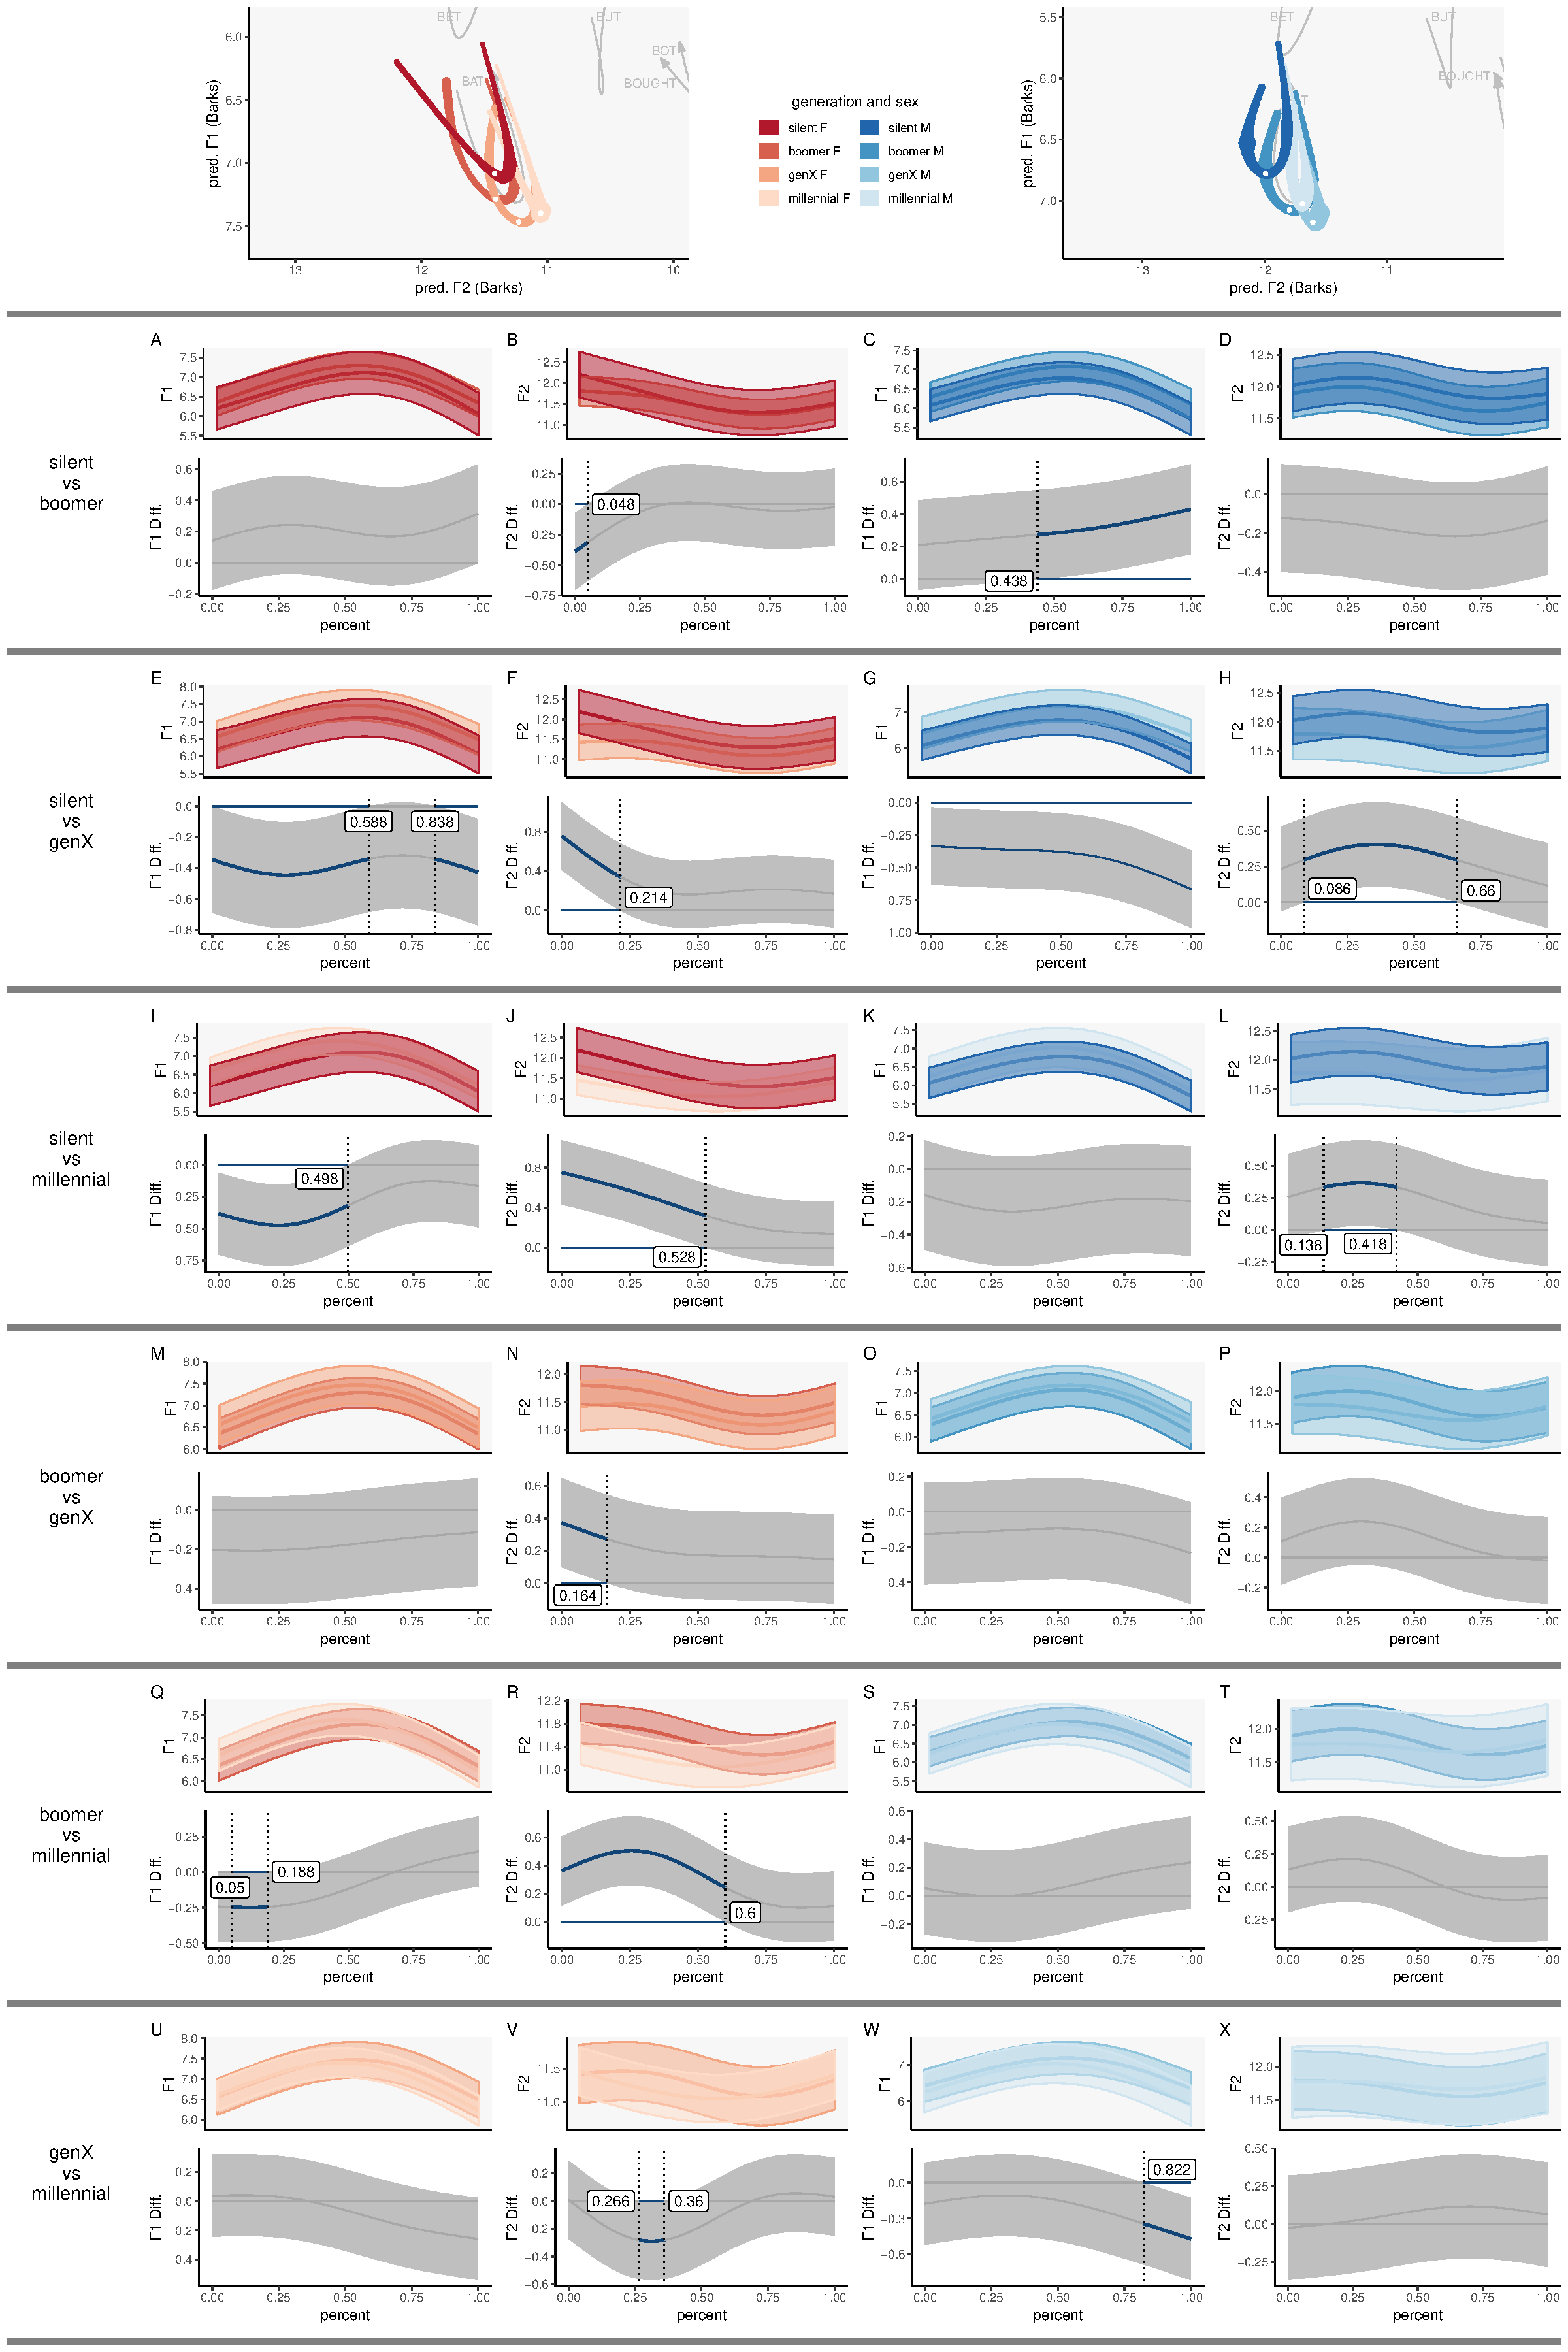
\includegraphics[width=\textwidth]{Figures/BAT/BAT_detailed_generation_panel_plot.pdf}
    \caption{Difference smooths comparing generation pairs for \bat.}
    \label{fig:bat_diff_smooths_gen}
\end{figure}

\begin{figure}[p]
    \centering
    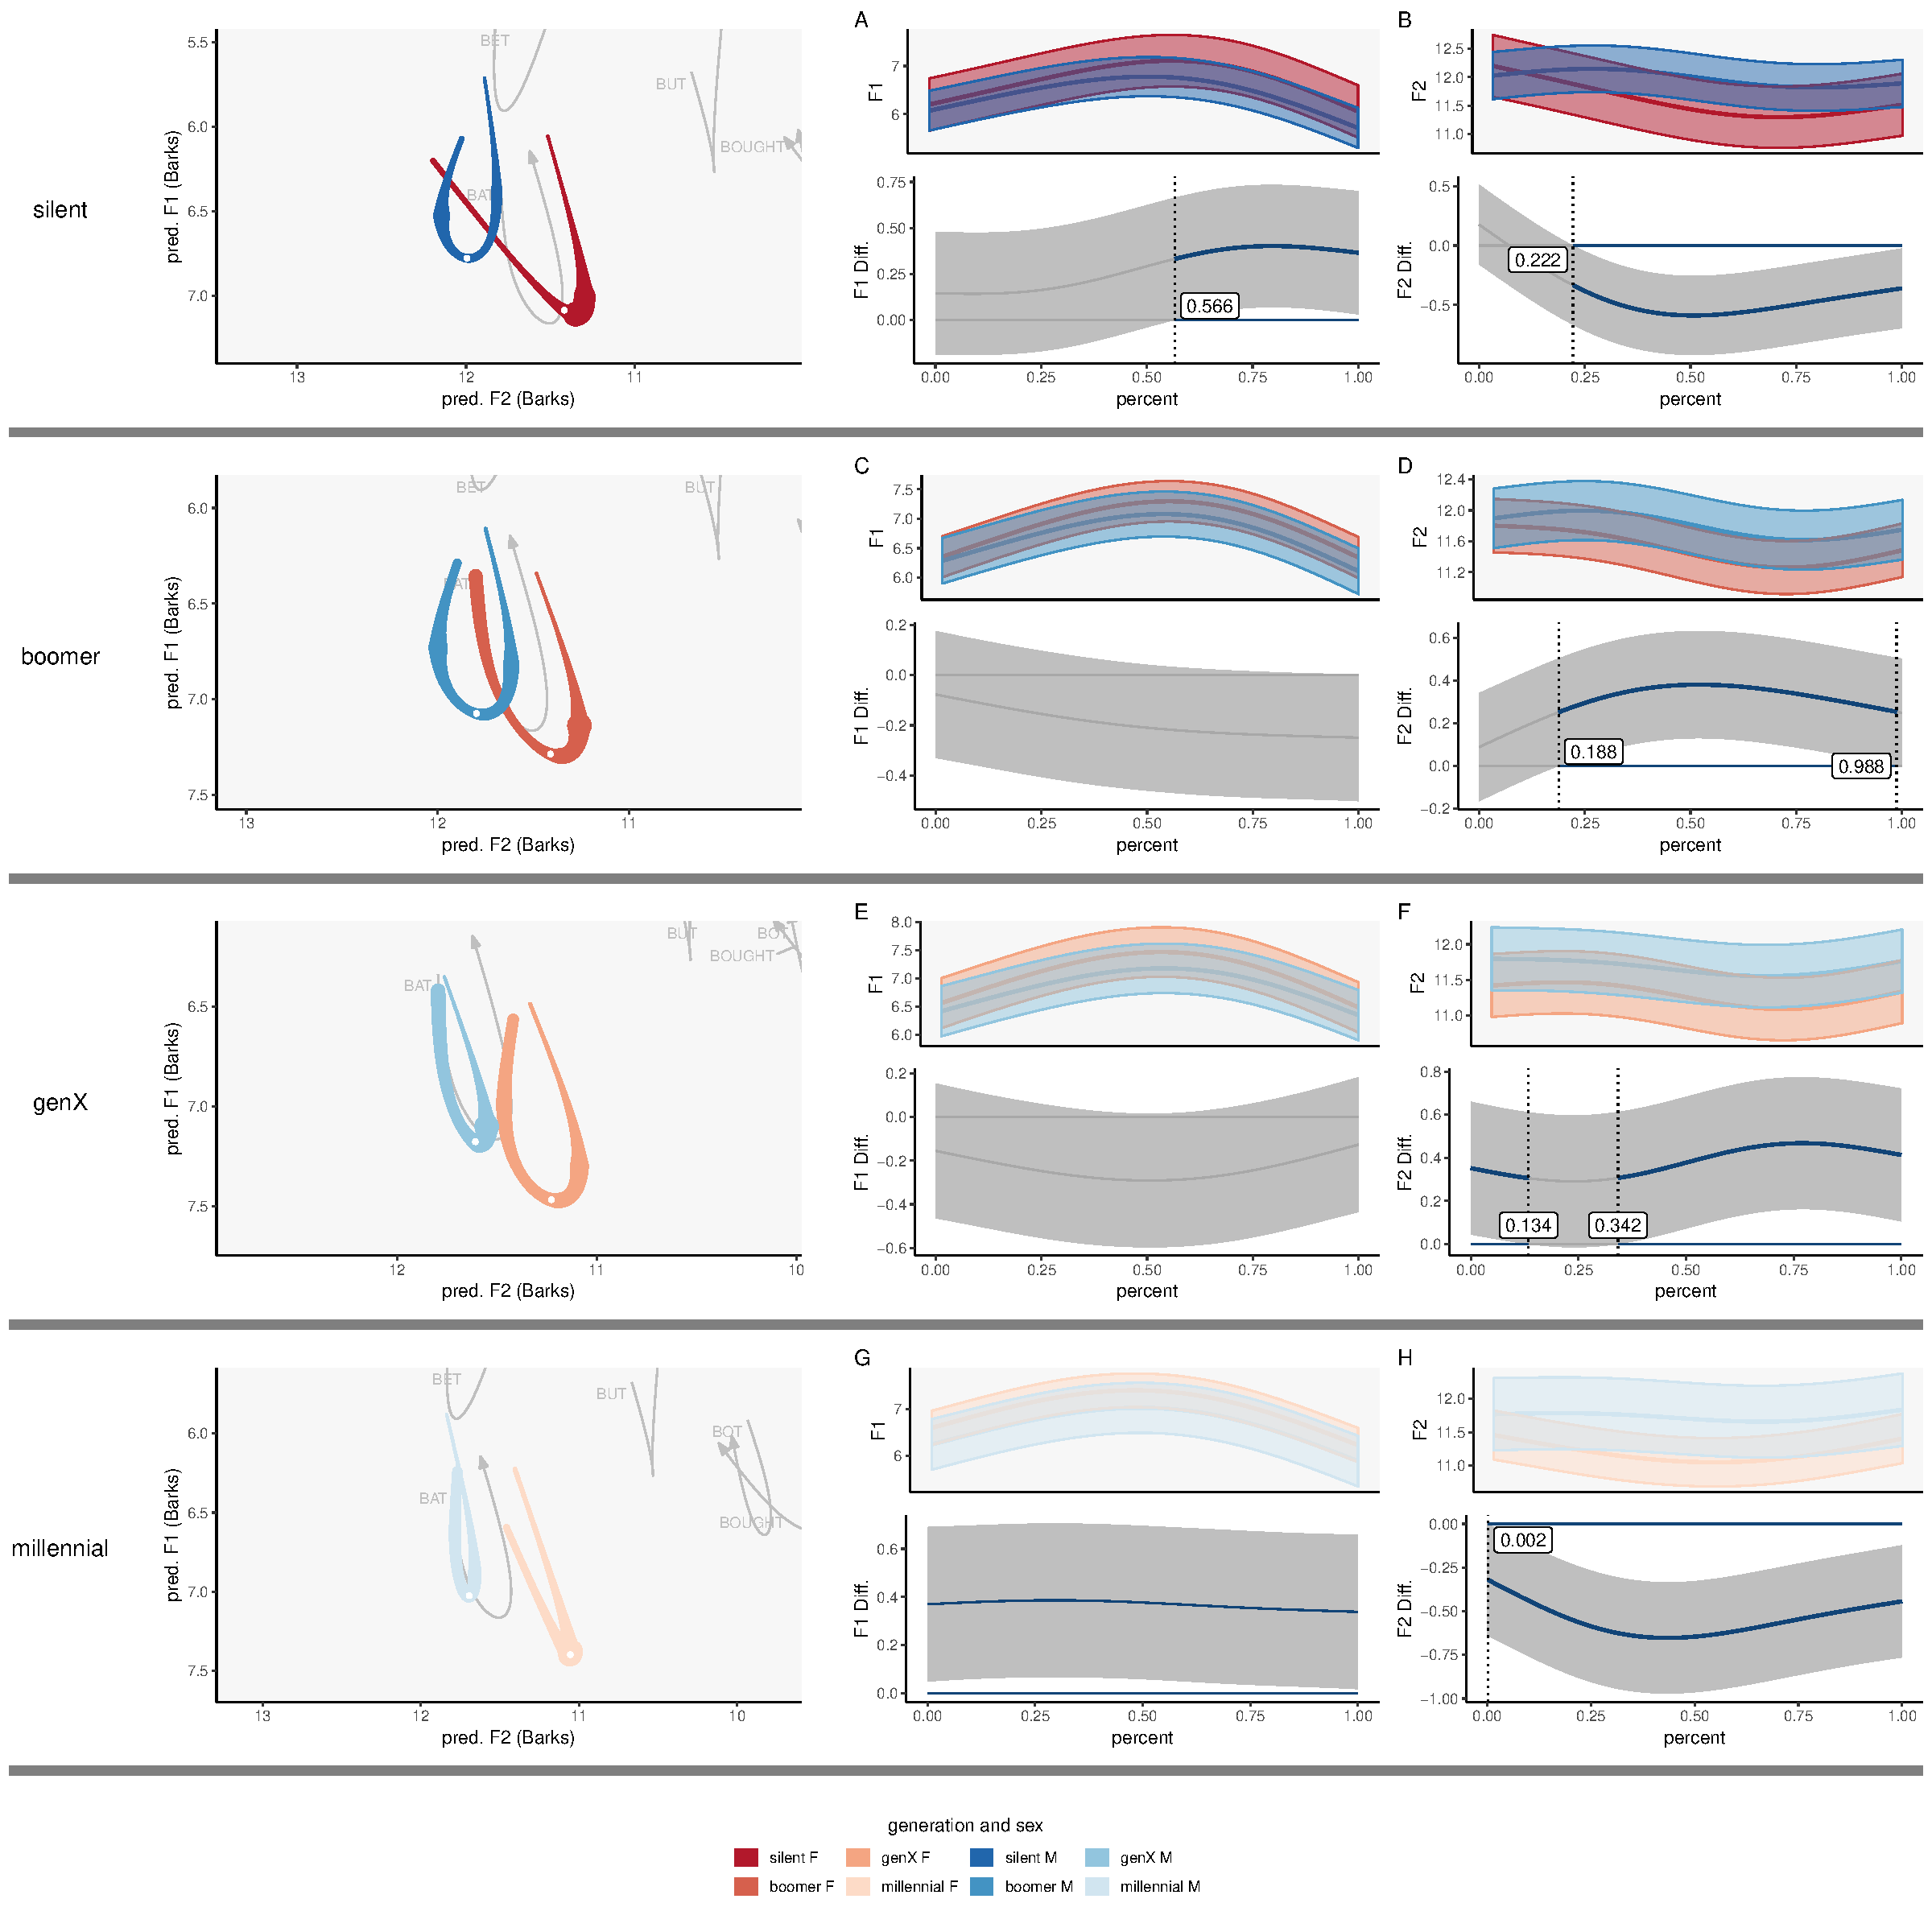
\includegraphics[width=\textwidth]{Figures/BAT/BAT_sex_panel_plot.pdf}
    \caption{Difference smooths comparing the sexes for \bat.}
    \label{fig:bat_diff_smooths_sex_gen}
\end{figure}


\begin{figure}[p]
    \centering
    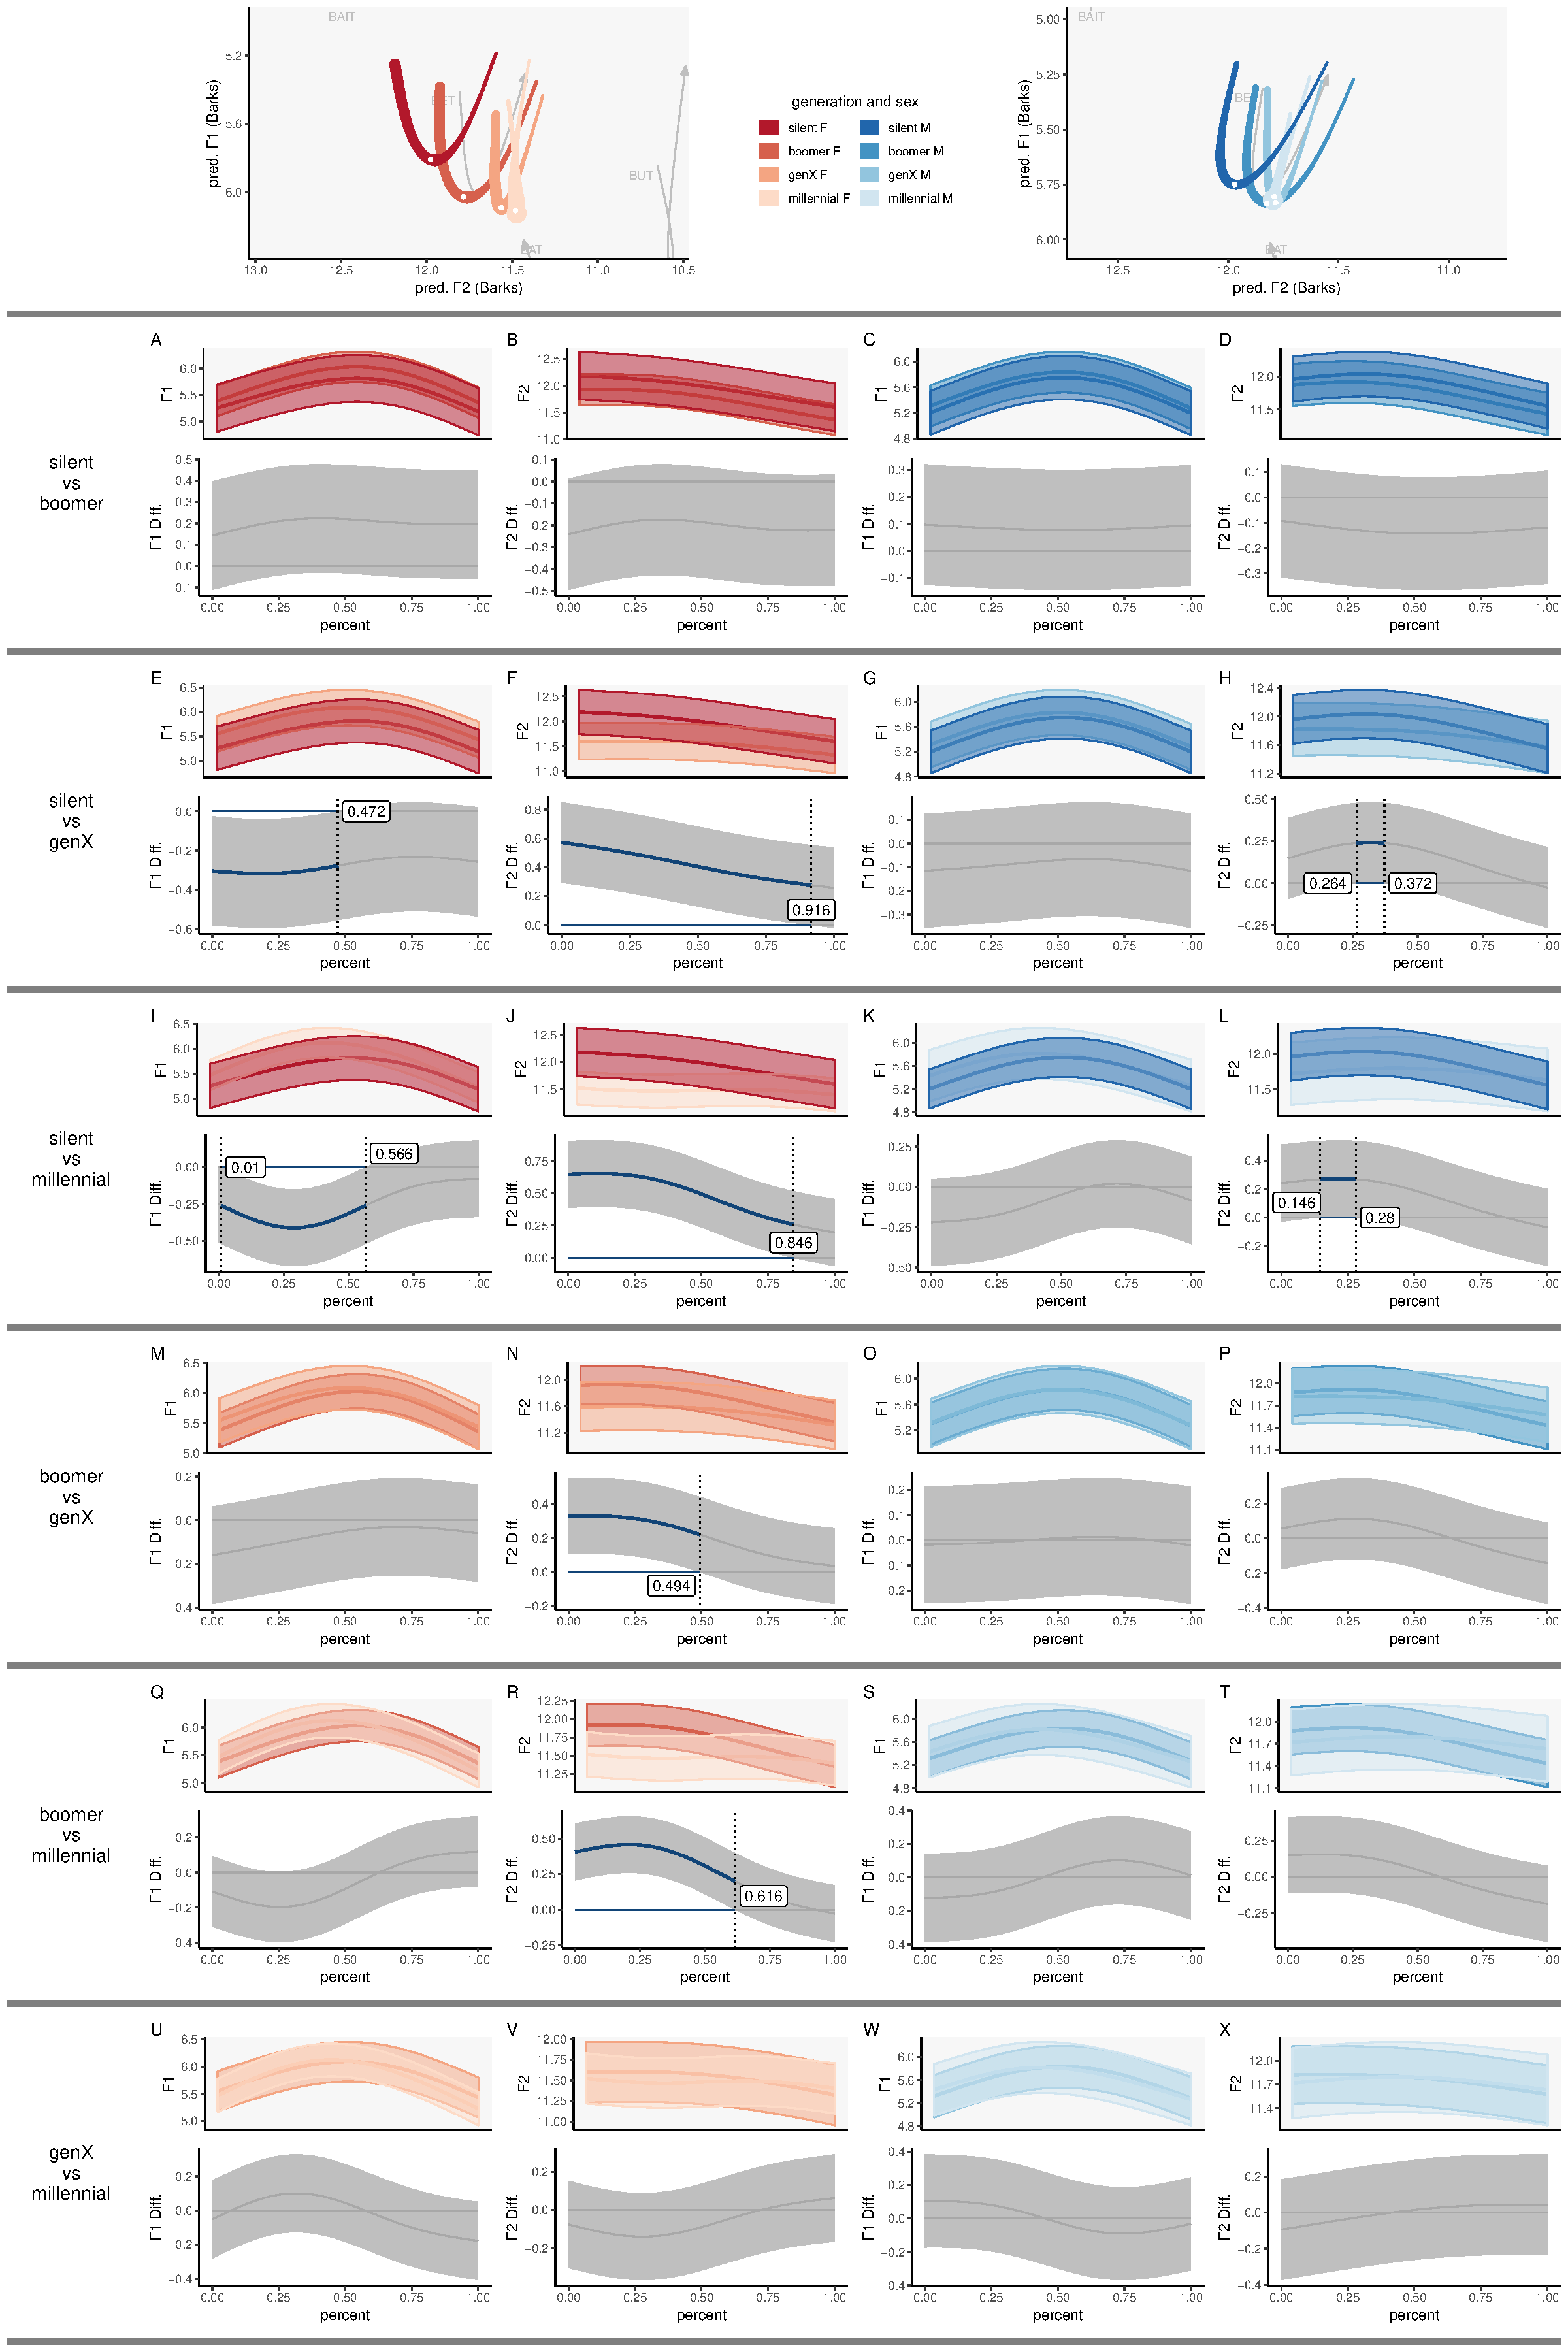
\includegraphics[width=\textwidth]{Figures/BET/BET_detailed_generation_panel_plot.pdf}
    \caption{Difference smooths comparing generation pairs for \bet.}
    \label{fig:bet_diff_smooths_gen}
\end{figure}

\begin{figure}[p]
    \centering
    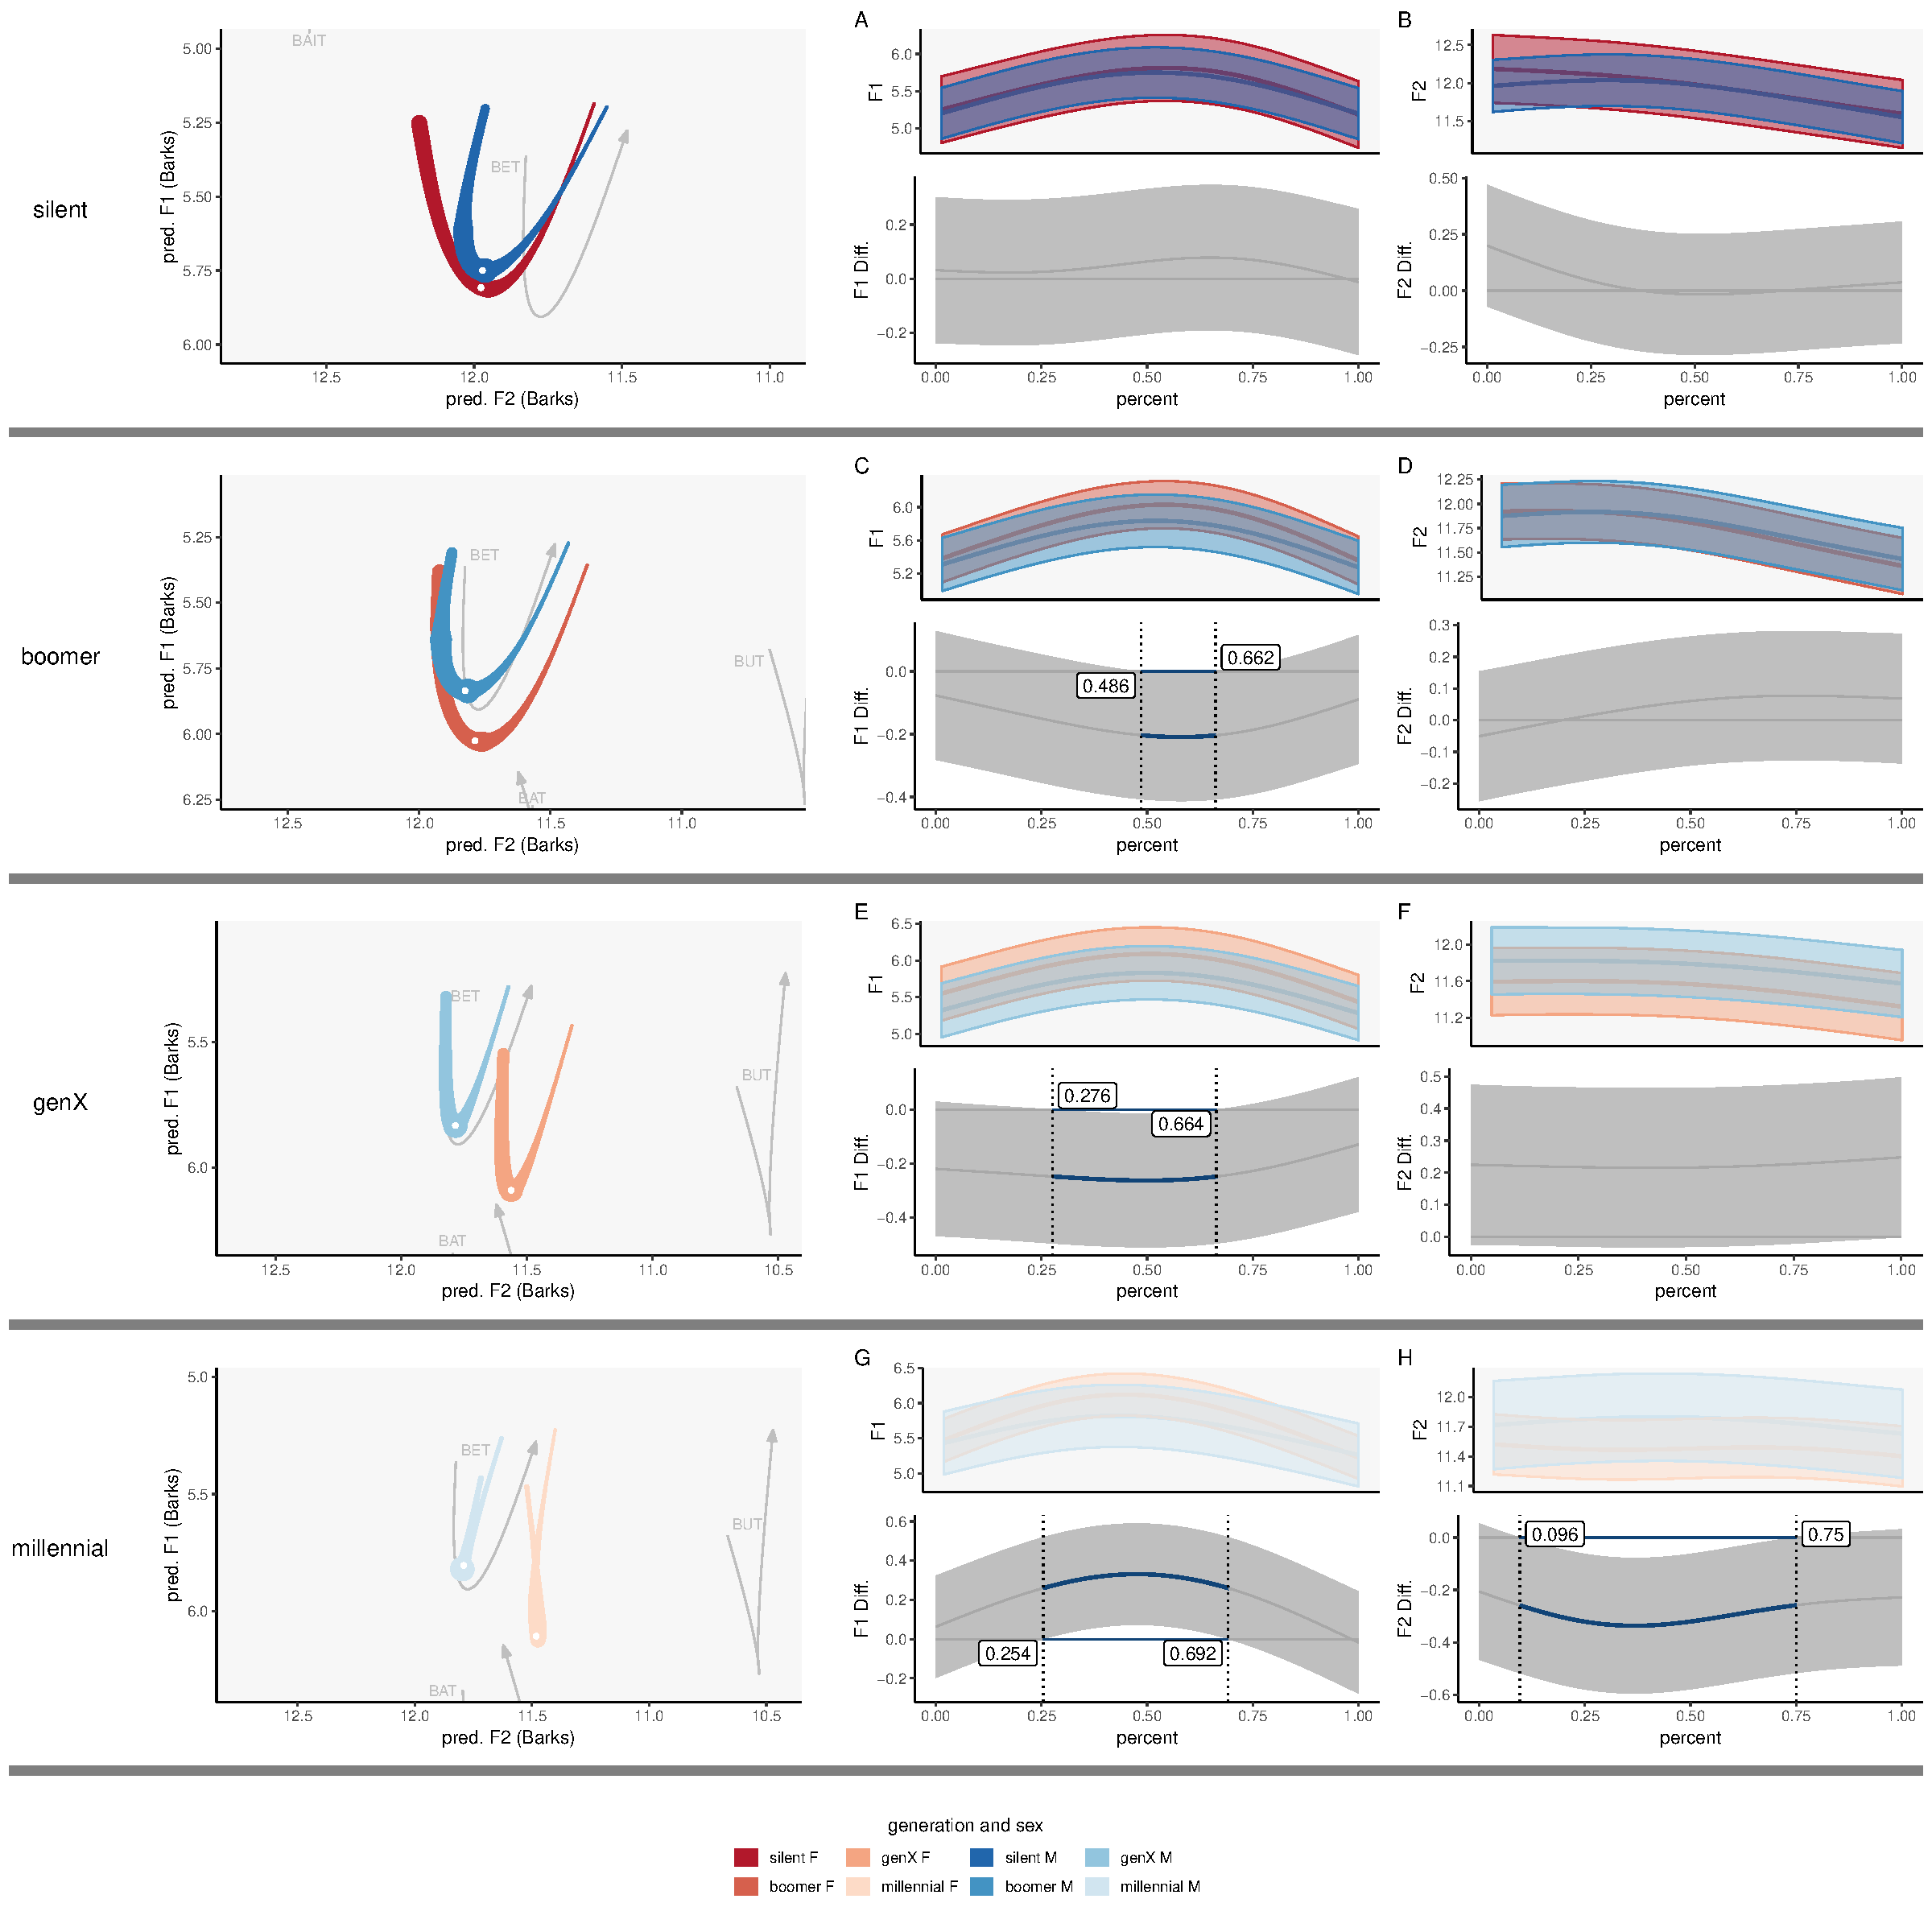
\includegraphics[width=\textwidth]{Figures/BET/BET_sex_panel_plot.pdf}
    \caption{Difference smooths comparing the sexes for \bet.}
    \label{fig:bet_diff_smooths_sex_gen}
\end{figure}



\begin{figure}[p]
    \centering
    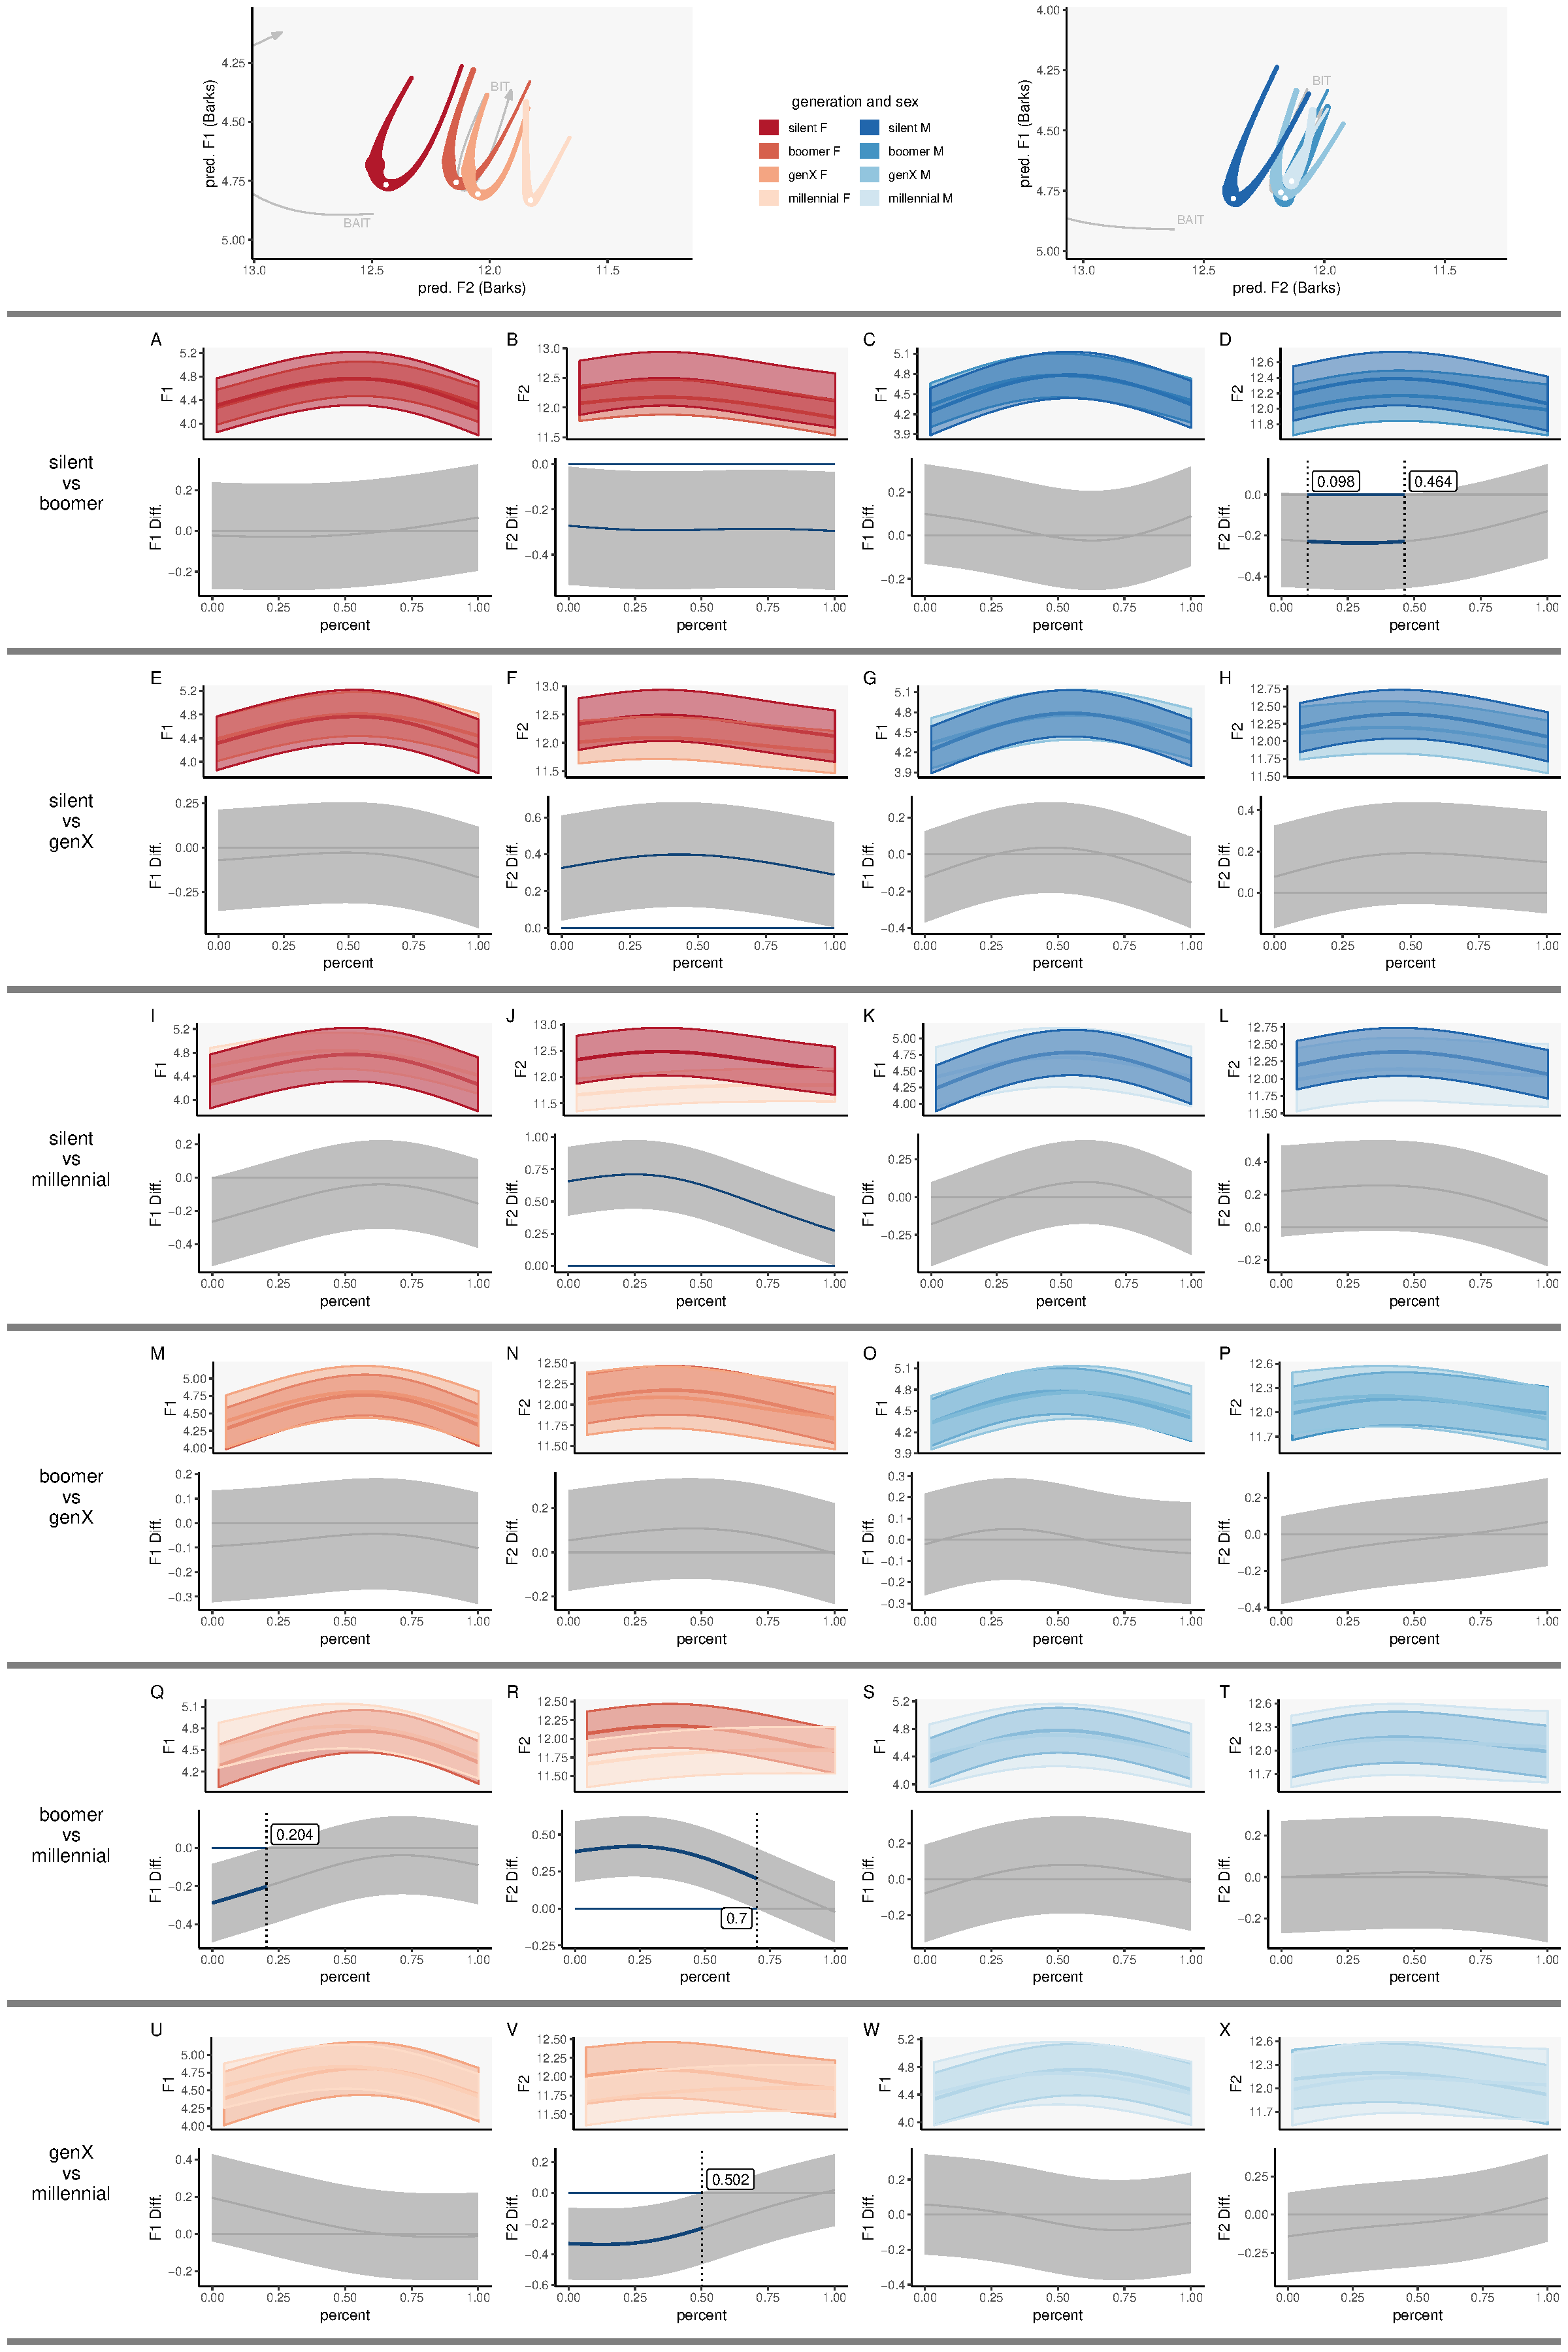
\includegraphics[width=\textwidth]{Figures/BIT/BIT_detailed_generation_panel_plot.pdf}
    \caption{Difference smooths comparing generation pairs for \bit.}
    \label{fig:bit_diff_smooths_gen}
\end{figure}

\begin{figure}[p]
    \centering
    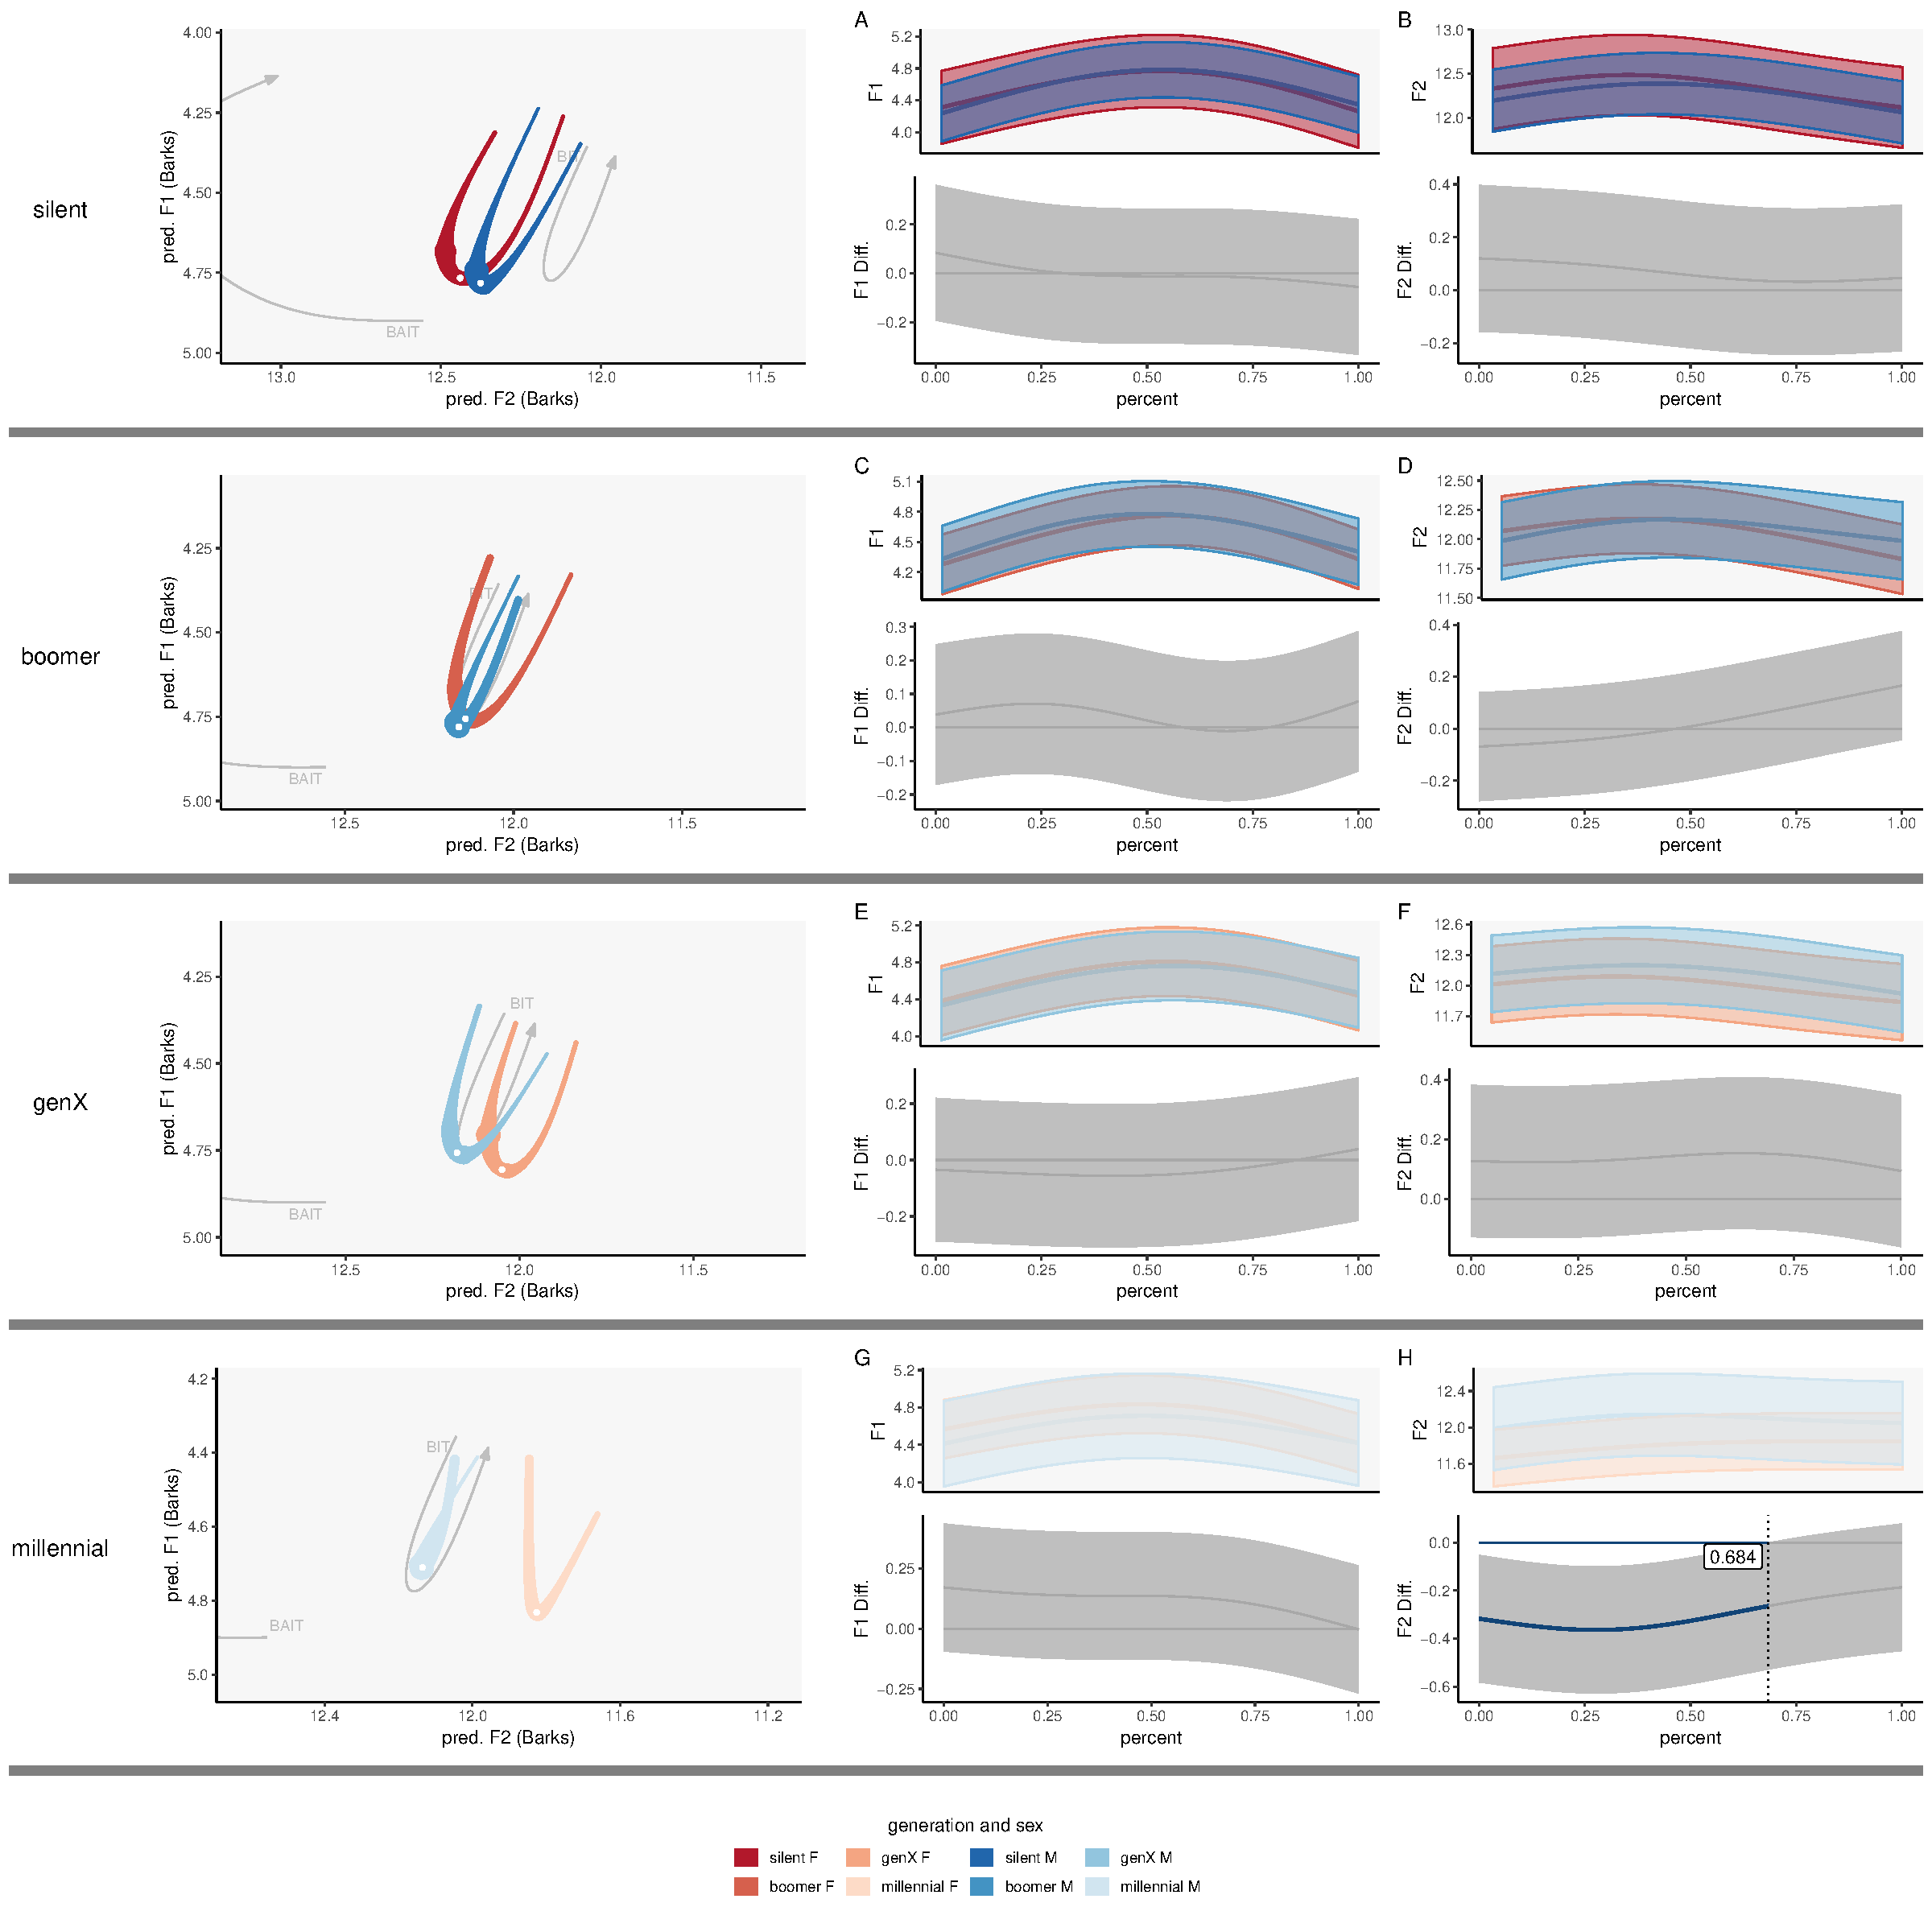
\includegraphics[width=\textwidth]{Figures/BIT/BIT_sex_panel_plot.pdf}
    \caption{Difference smooths comparing the sexes for \bit.}
    \label{fig:bit_diff_smooths_sex_gen}
\end{figure}



\begin{figure}[p]
    \centering
    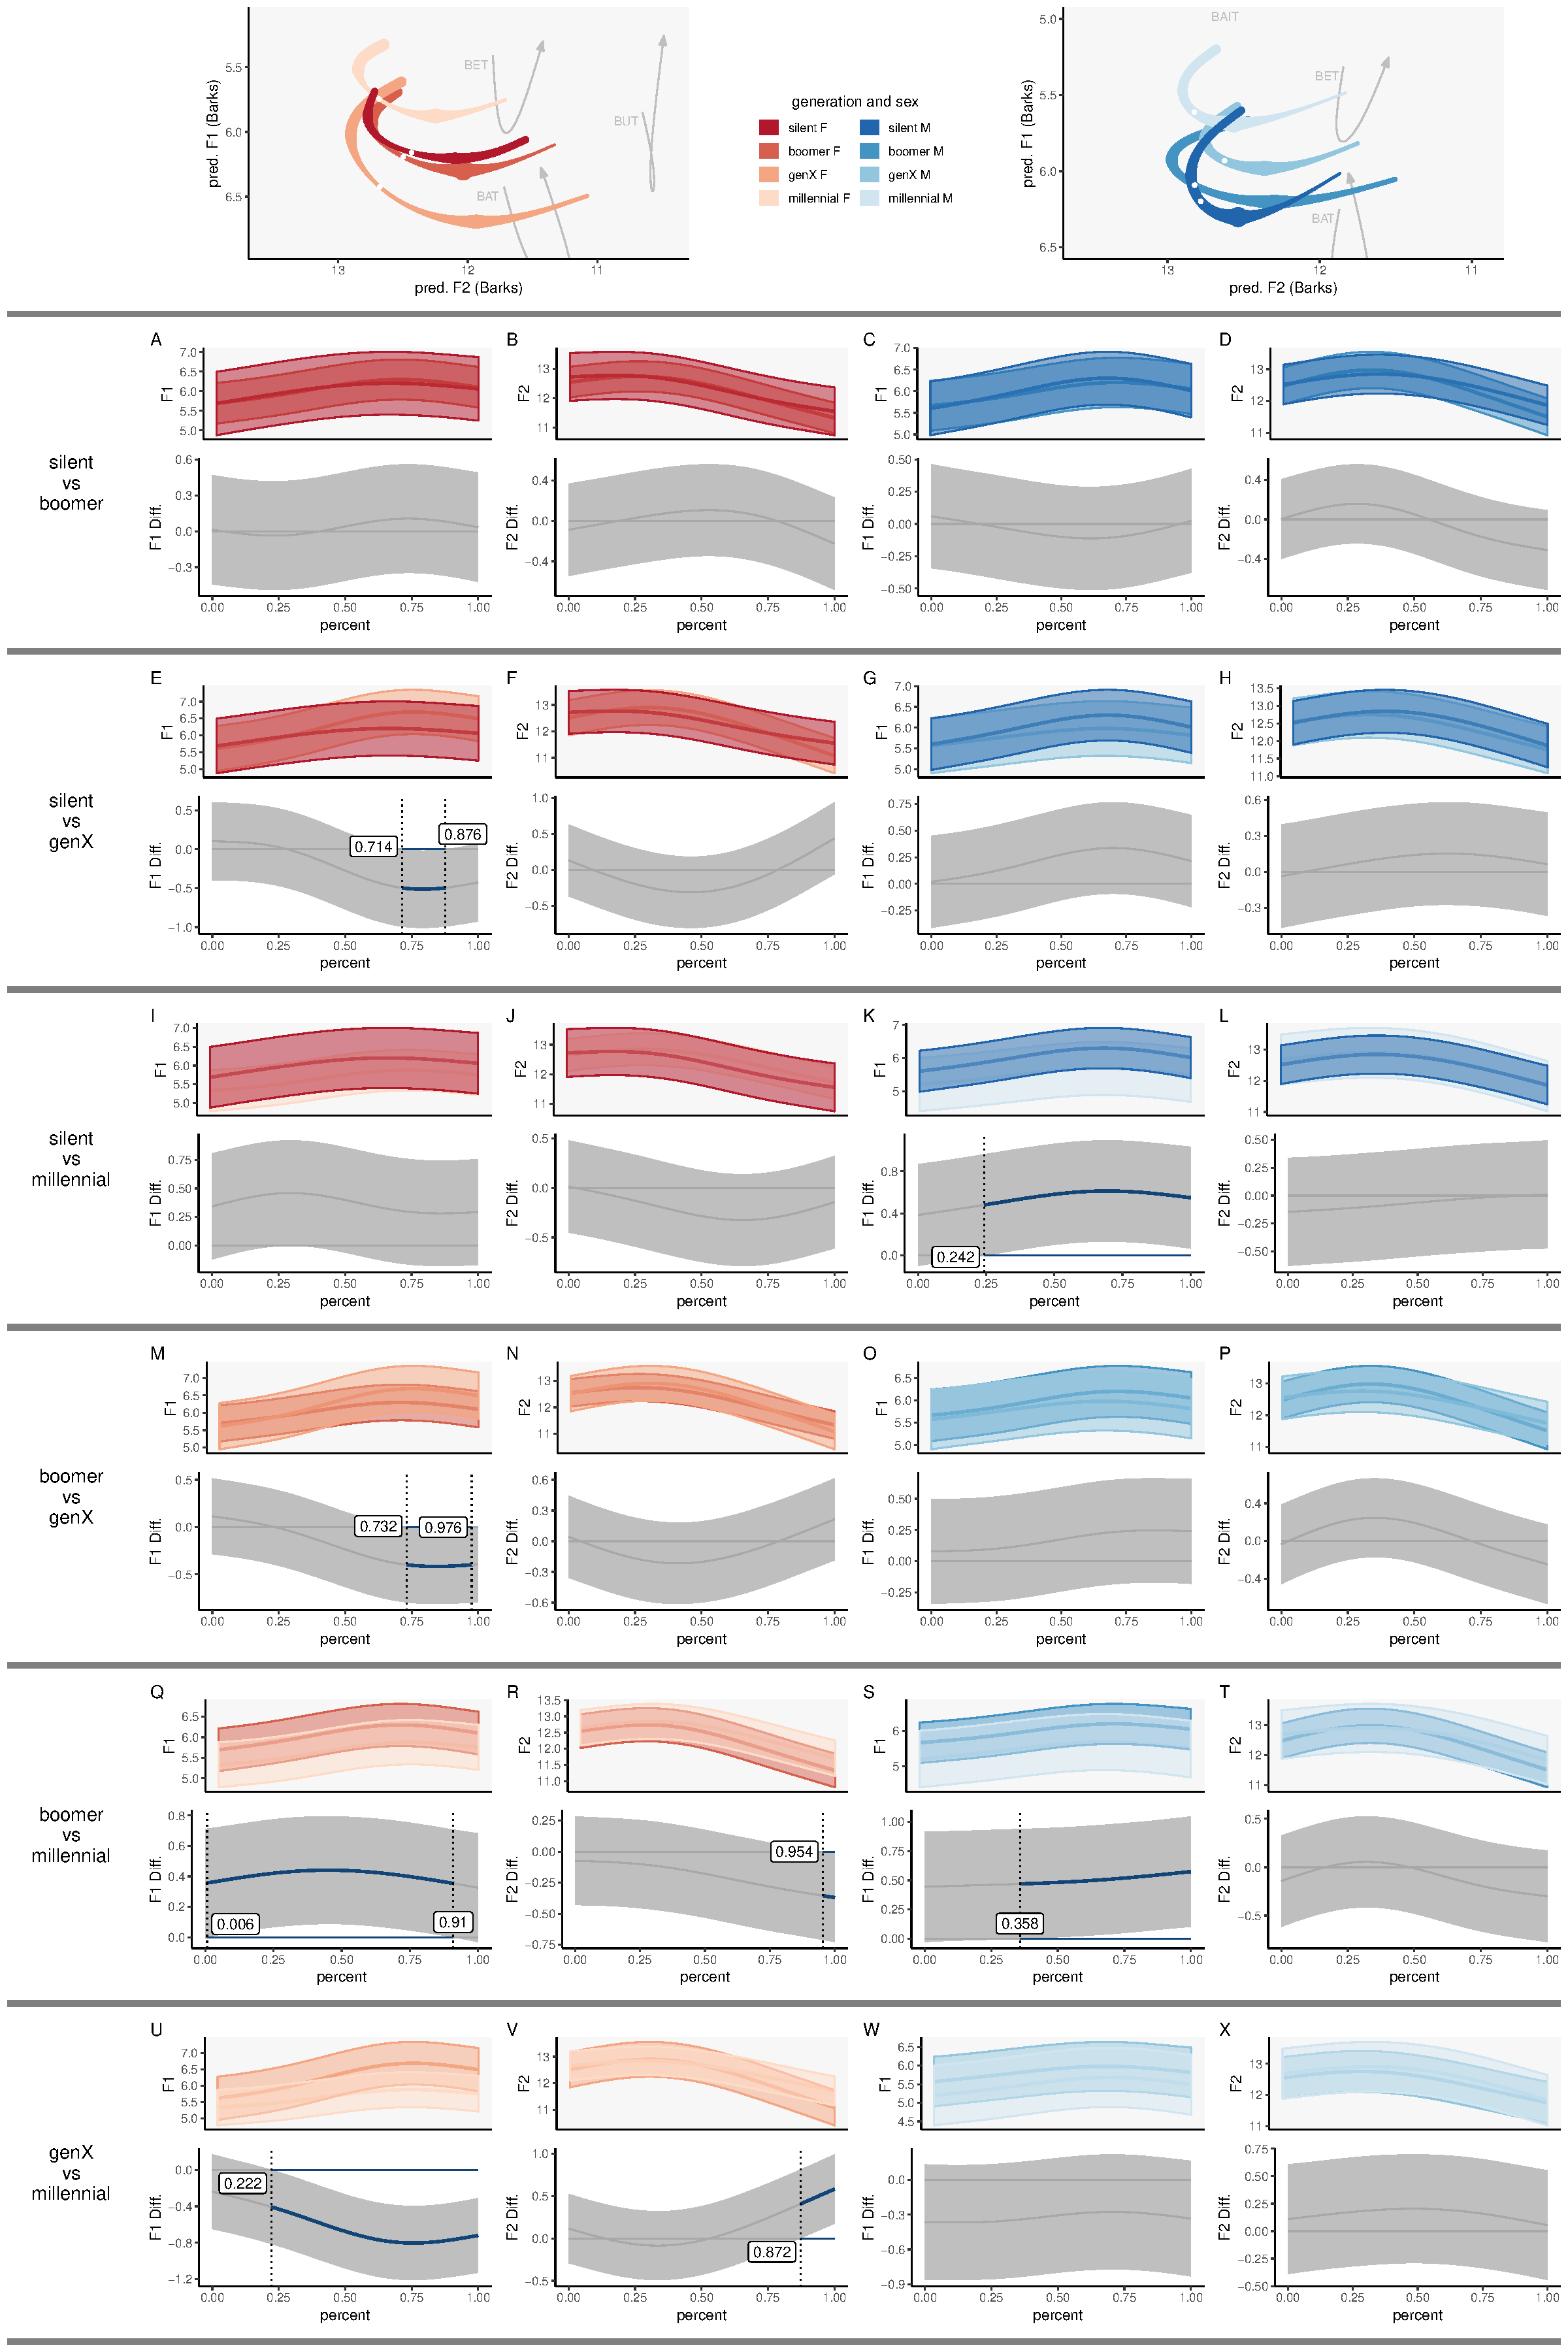
\includegraphics[width=\textwidth]{Figures/BAN/BAN_detailed_generation_panel_plot.pdf}
    \caption{Difference smooths comparing generation pairs for \ban.}
    \label{fig:ban_diff_smooths_gen}
\end{figure}

\begin{figure}[p]
    \centering
    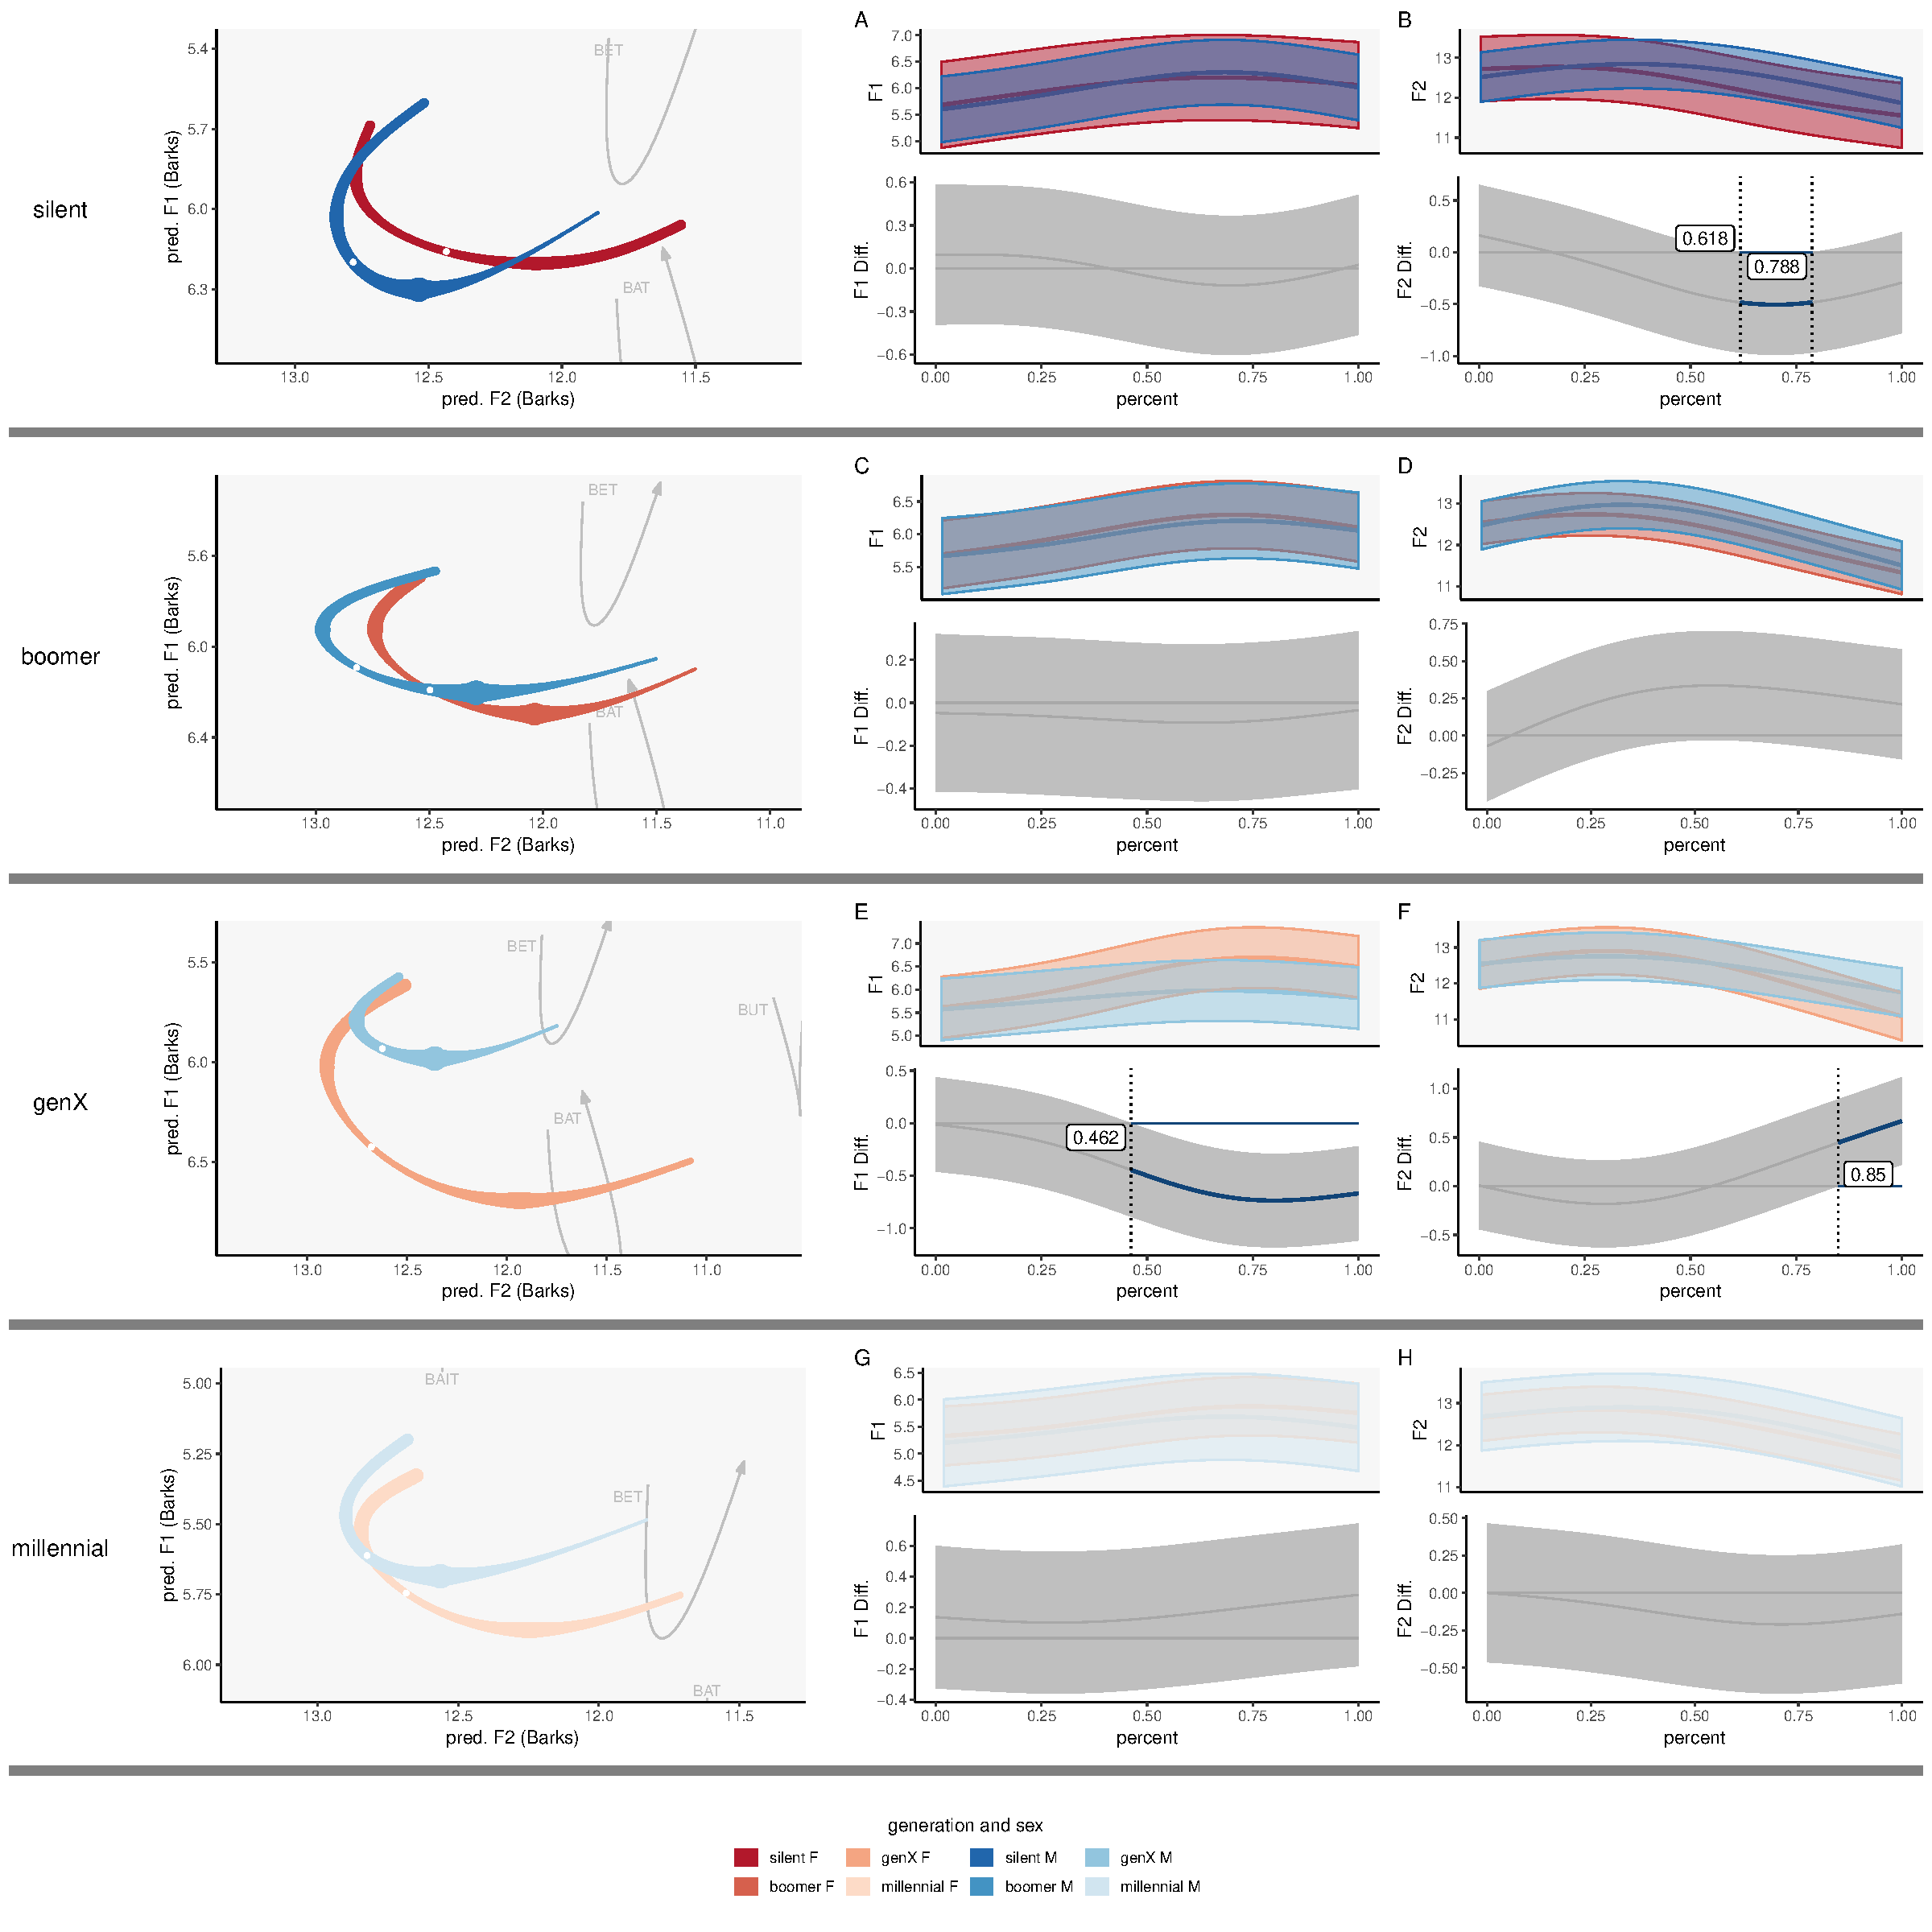
\includegraphics[width=\textwidth]{Figures/BAN/BAN_sex_panel_plot.pdf}
    \caption{Difference smooths comparing the sexes for \ban.}
    \label{fig:ban_diff_smooths_sex_gen}
\end{figure}



\begin{figure}[p]
    \centering
    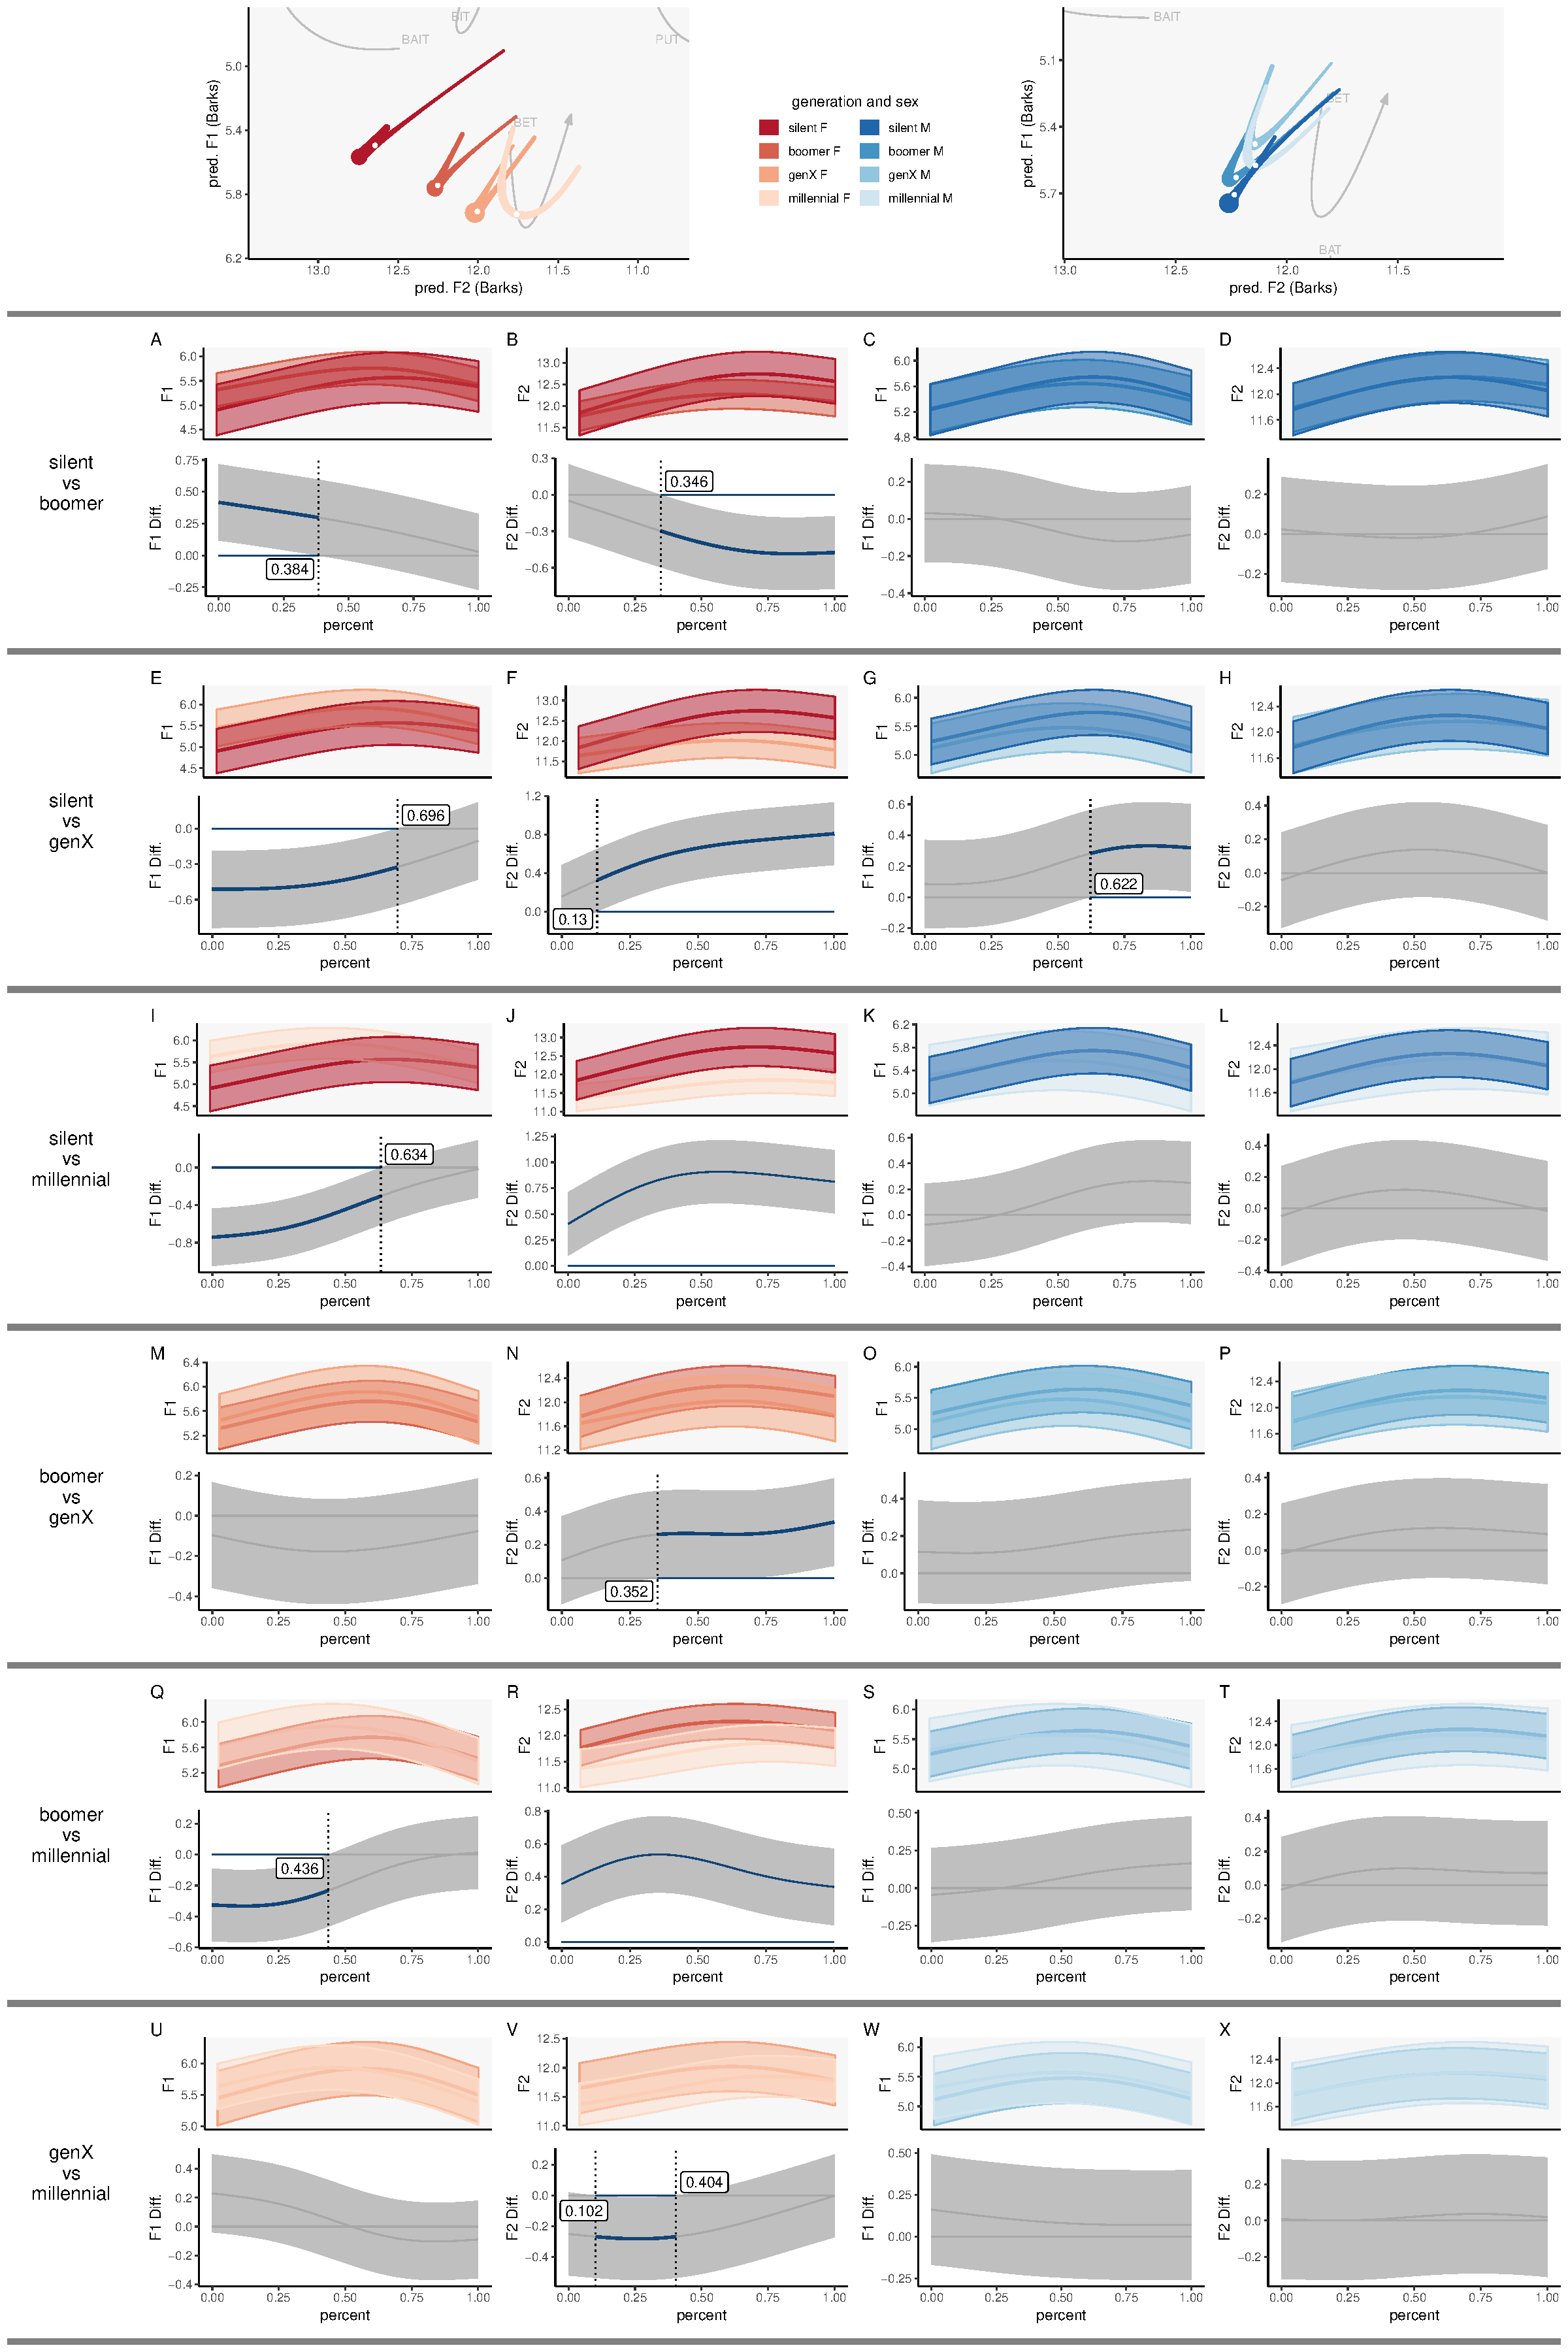
\includegraphics[width=\textwidth]{Figures/BEN/BEN_detailed_generation_panel_plot.pdf}
    \caption{Difference smooths comparing generation pairs for \ben.}
    \label{fig:ben_diff_smooths_gen}
\end{figure}

\begin{figure}[p]
    \centering
    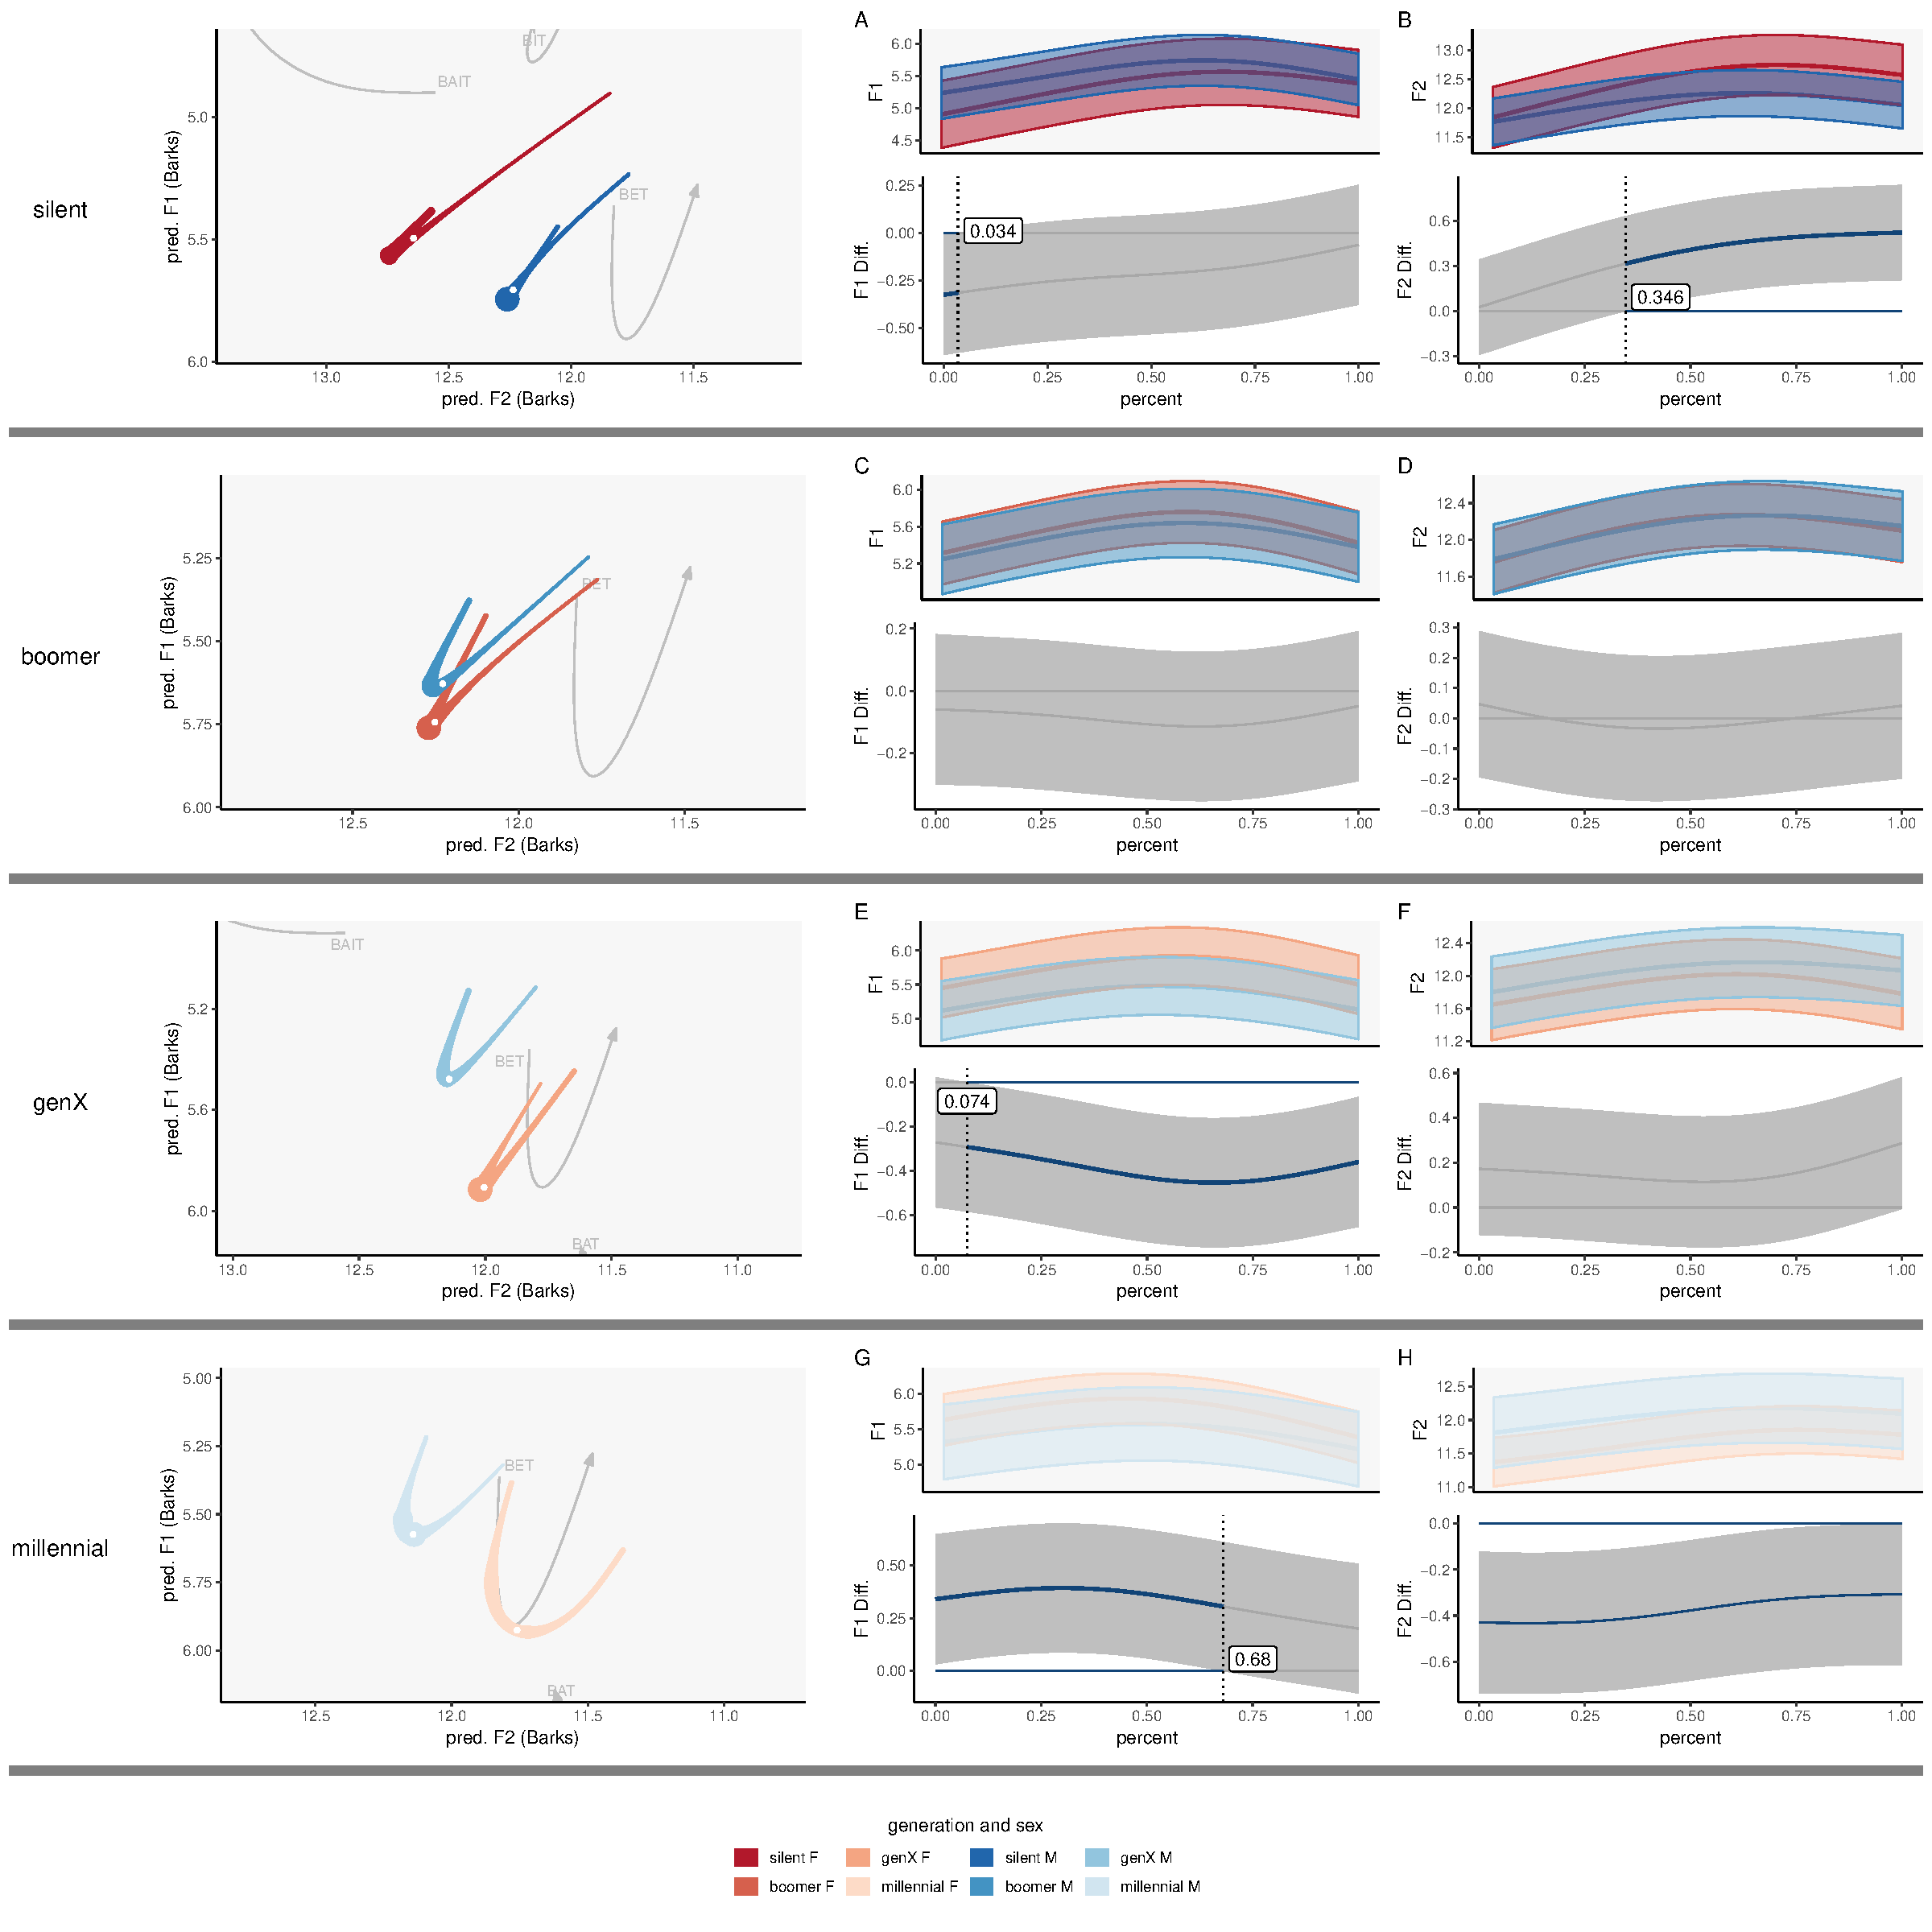
\includegraphics[width=\textwidth]{Figures/BEN/BEN_sex_panel_plot.pdf}
    \caption{Difference smooths comparing the sexes for \ben.}
    \label{fig:ben_diff_smooths_sex_gen}
\end{figure}



\begin{figure}[p]
    \centering
    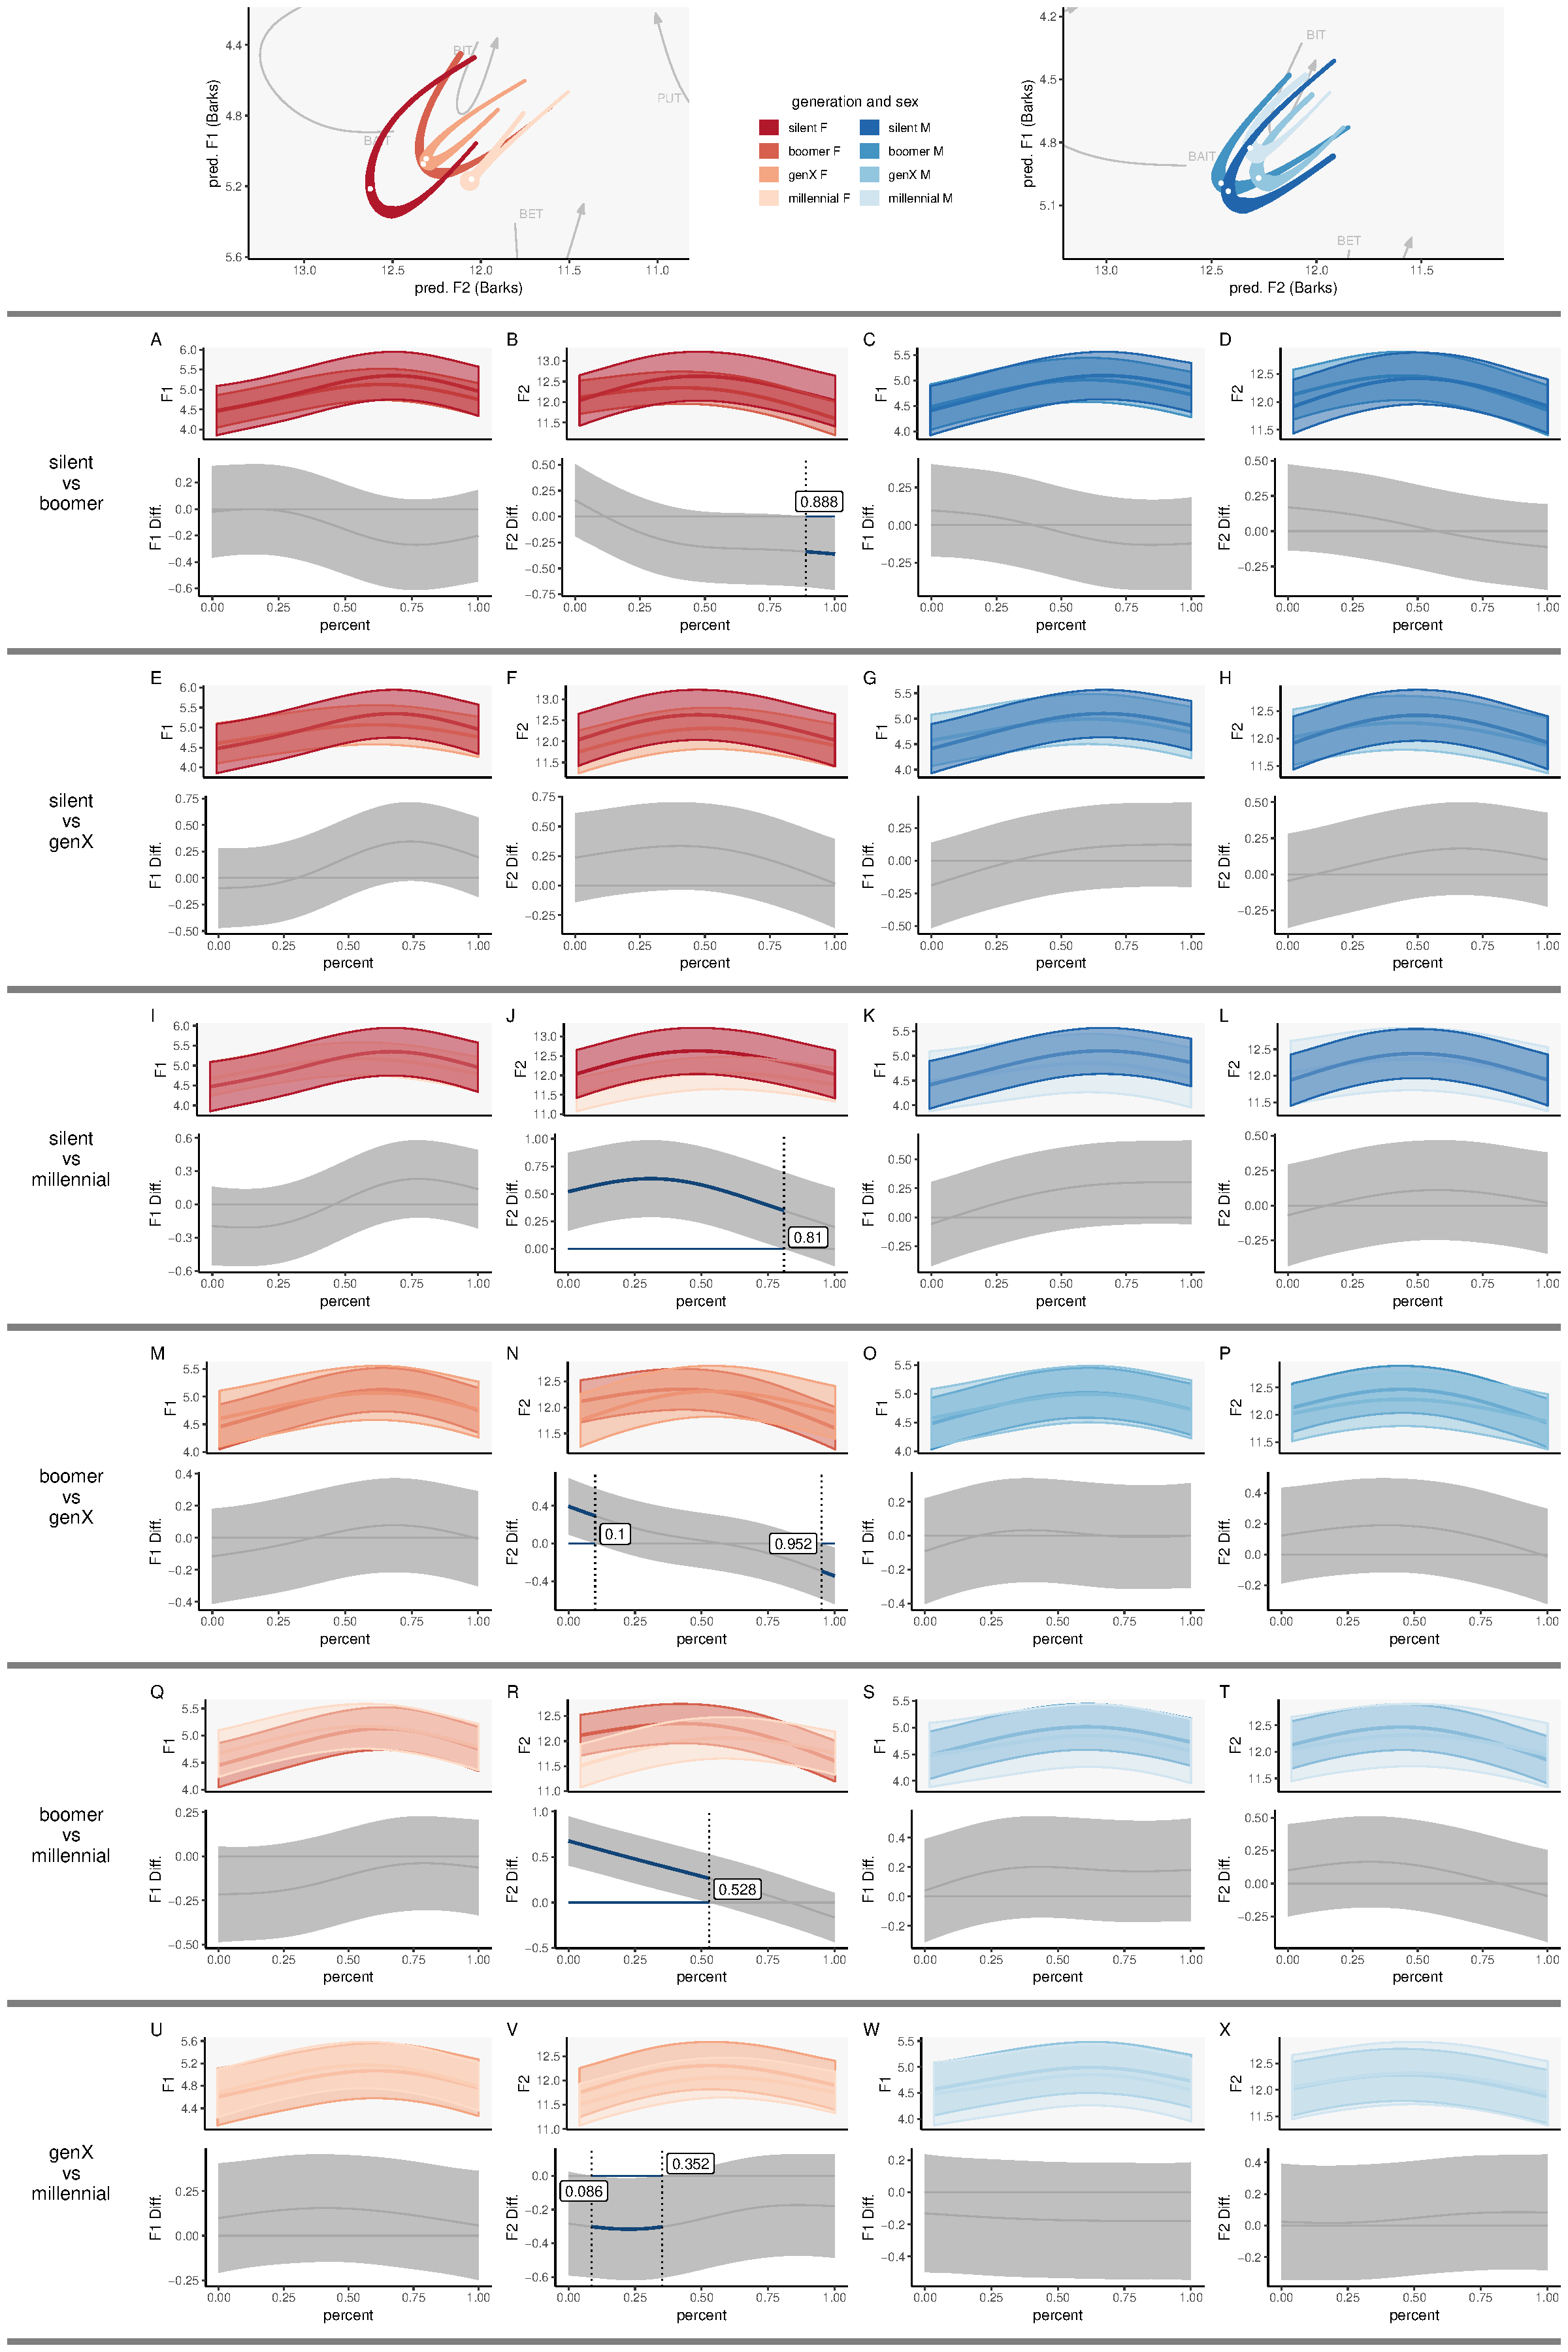
\includegraphics[width=\textwidth]{Figures/BIN/BIN_detailed_generation_panel_plot.pdf}
    \caption{Difference smooths comparing generation pairs for \bin.}
    \label{fig:bin_diff_smooths_gen}
\end{figure}

\begin{figure}[p]
    \centering
    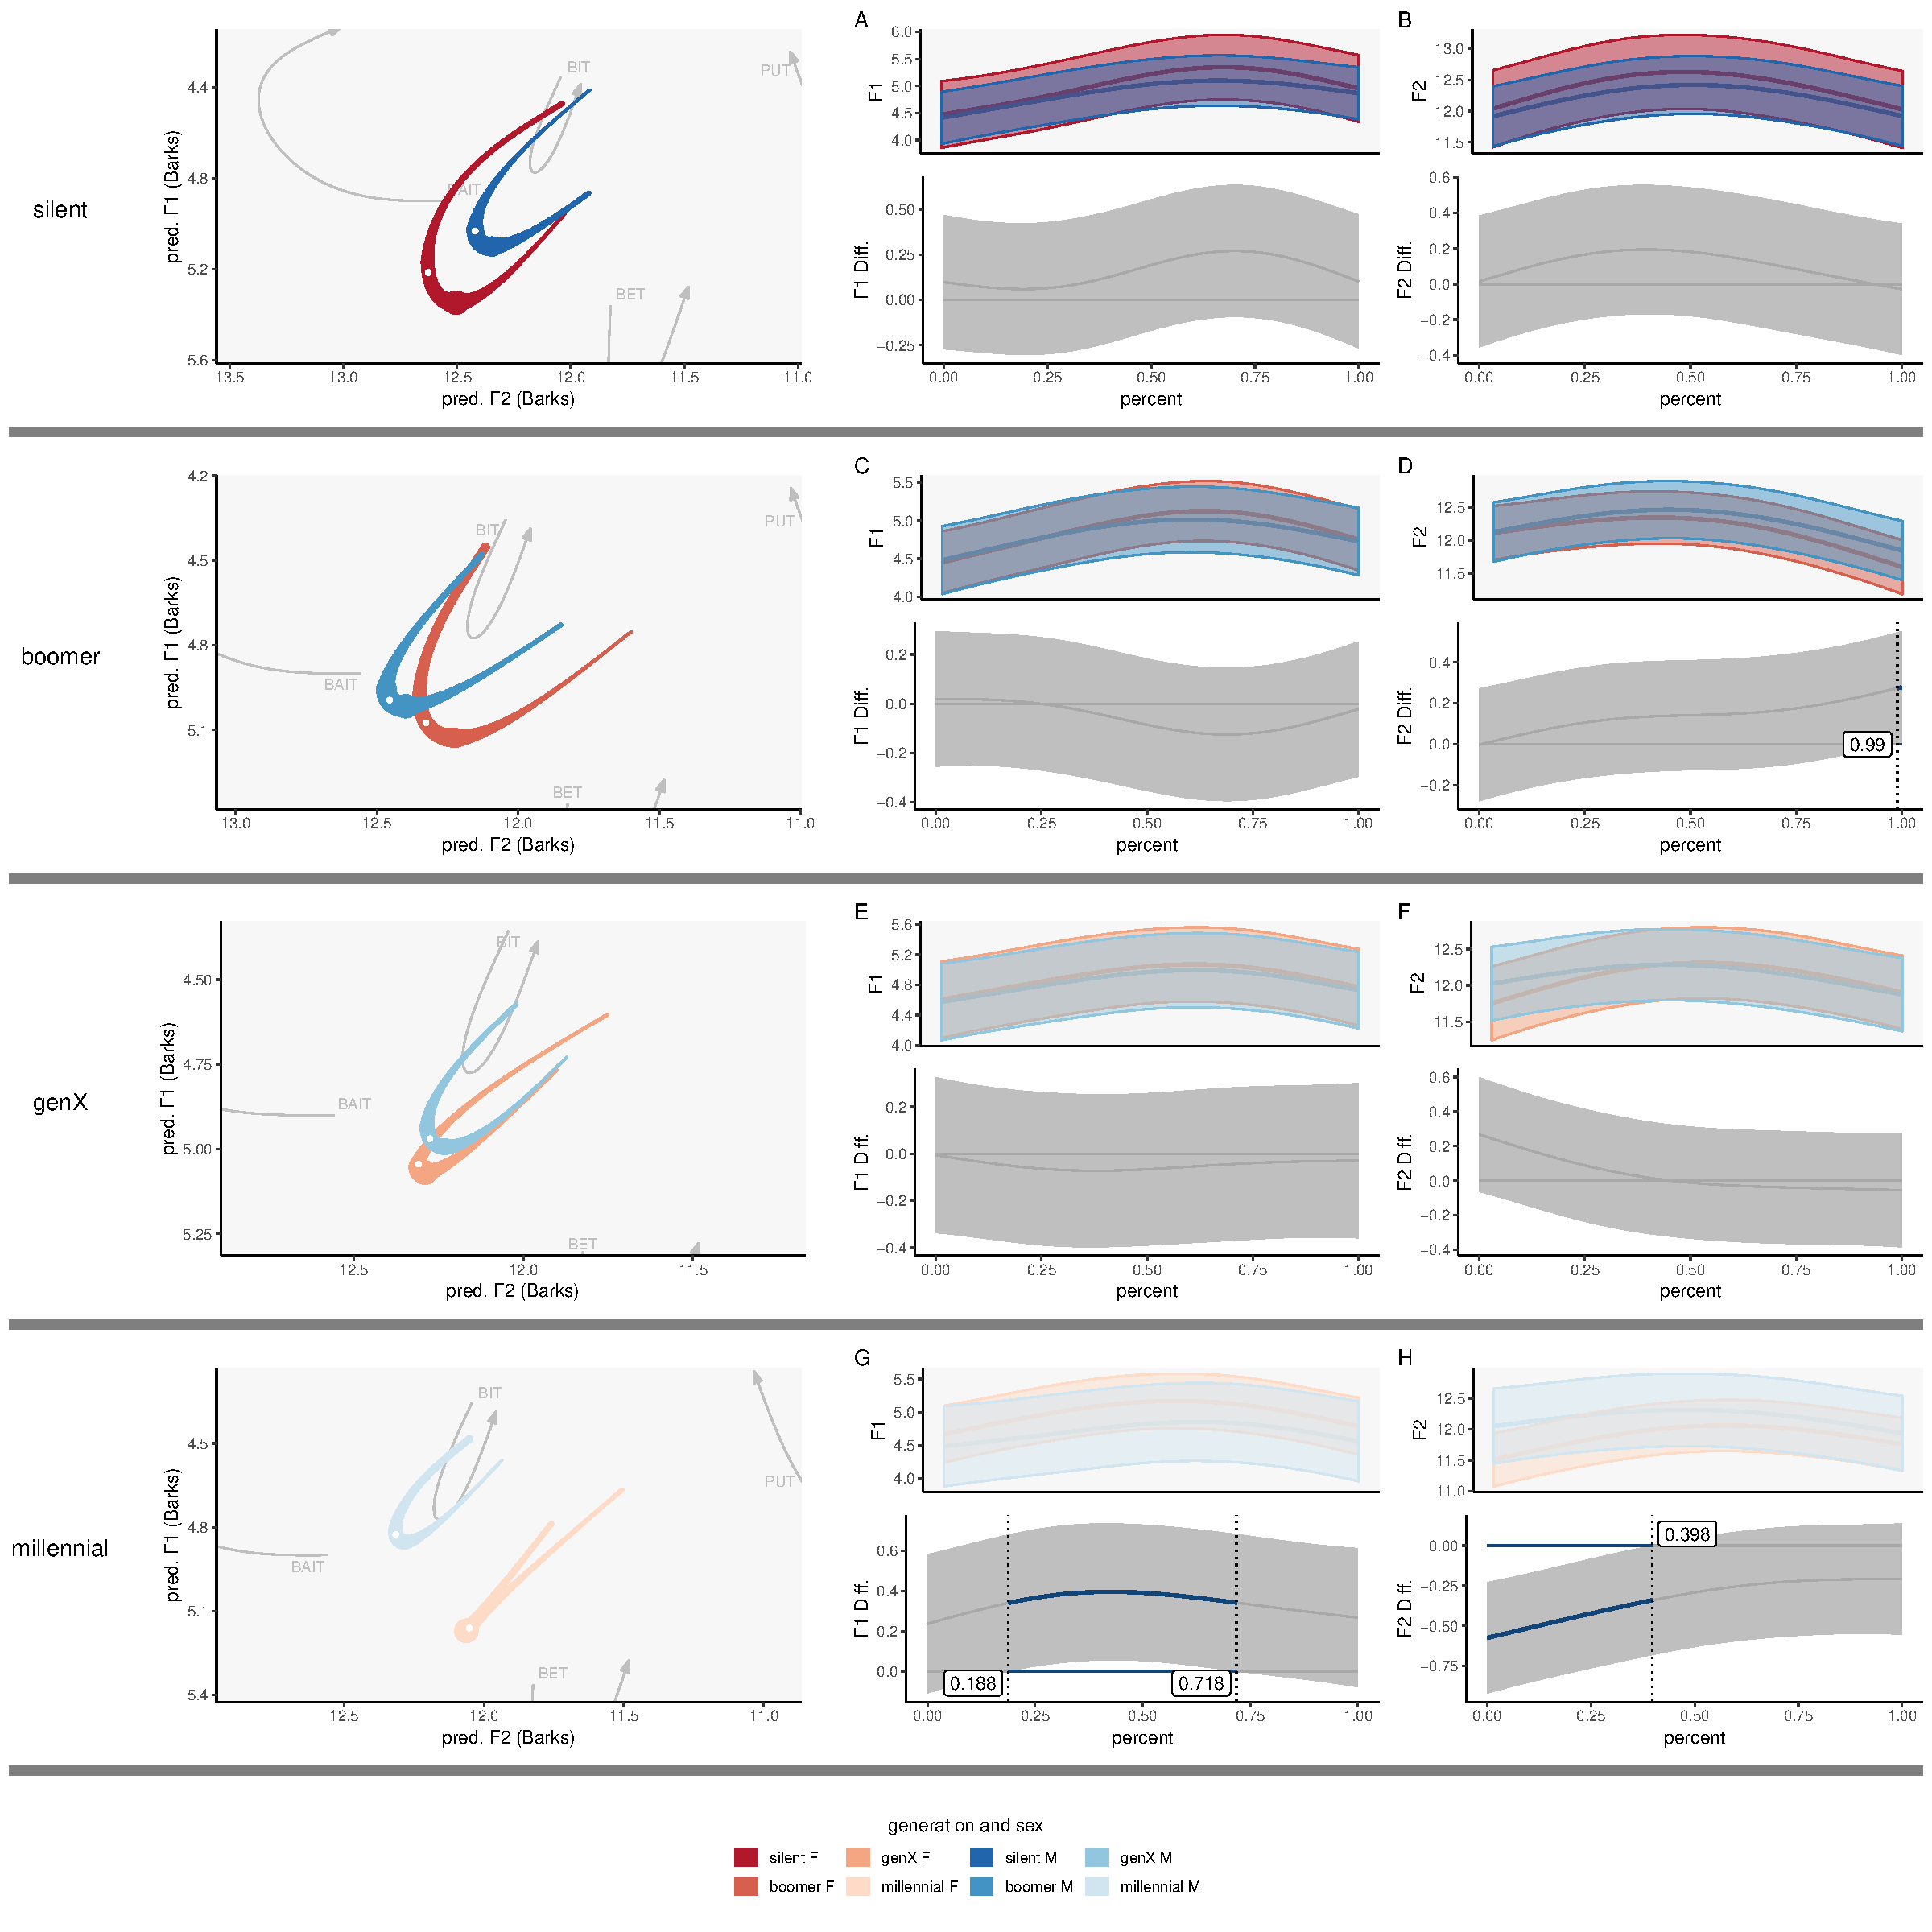
\includegraphics[width=\textwidth]{Figures/BIN/BIN_sex_panel_plot.pdf}
    \caption{Difference smooths comparing the sexes for \bin.}
    \label{fig:bin_diff_smooths_sex_gen}
\end{figure}




\begin{figure}[p]
    \centering
    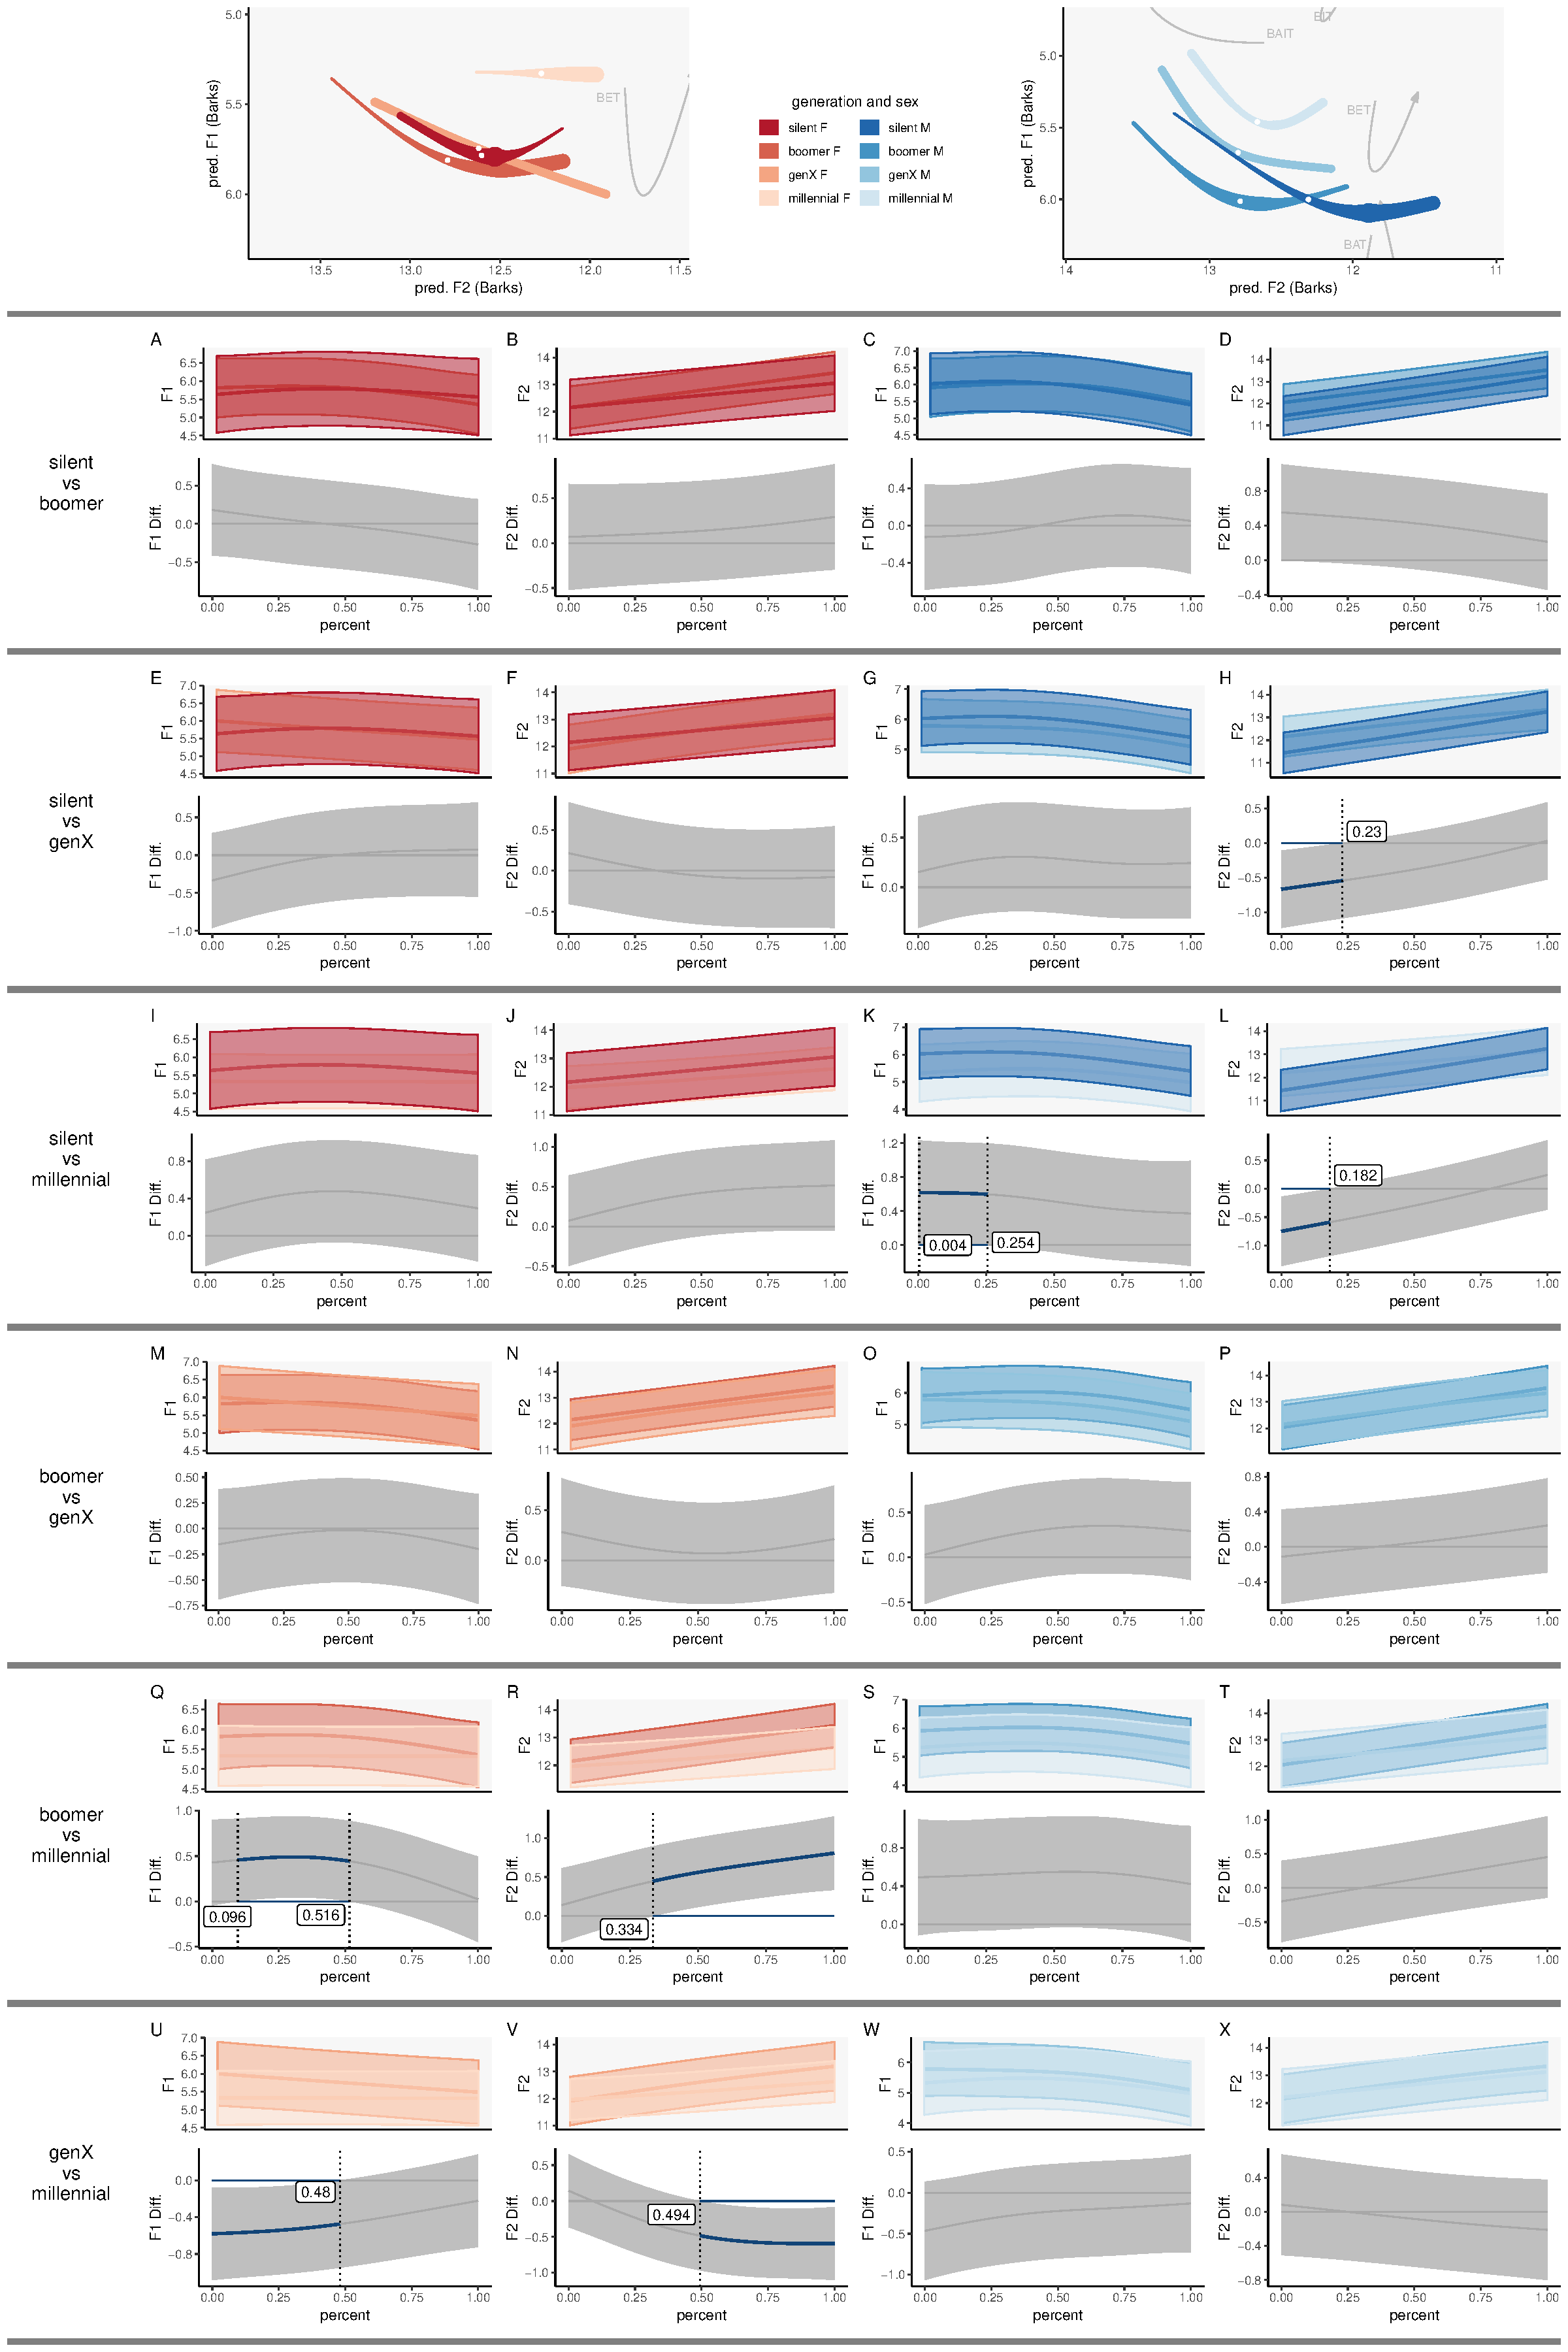
\includegraphics[width=\textwidth]{Figures/BANG/BANG_detailed_generation_panel_plot.pdf}
    \caption{Difference smooths comparing generation pairs for \bang.}
    \label{fig:bang_diff_smooths_gen}
\end{figure}

\begin{figure}[p]
    \centering
    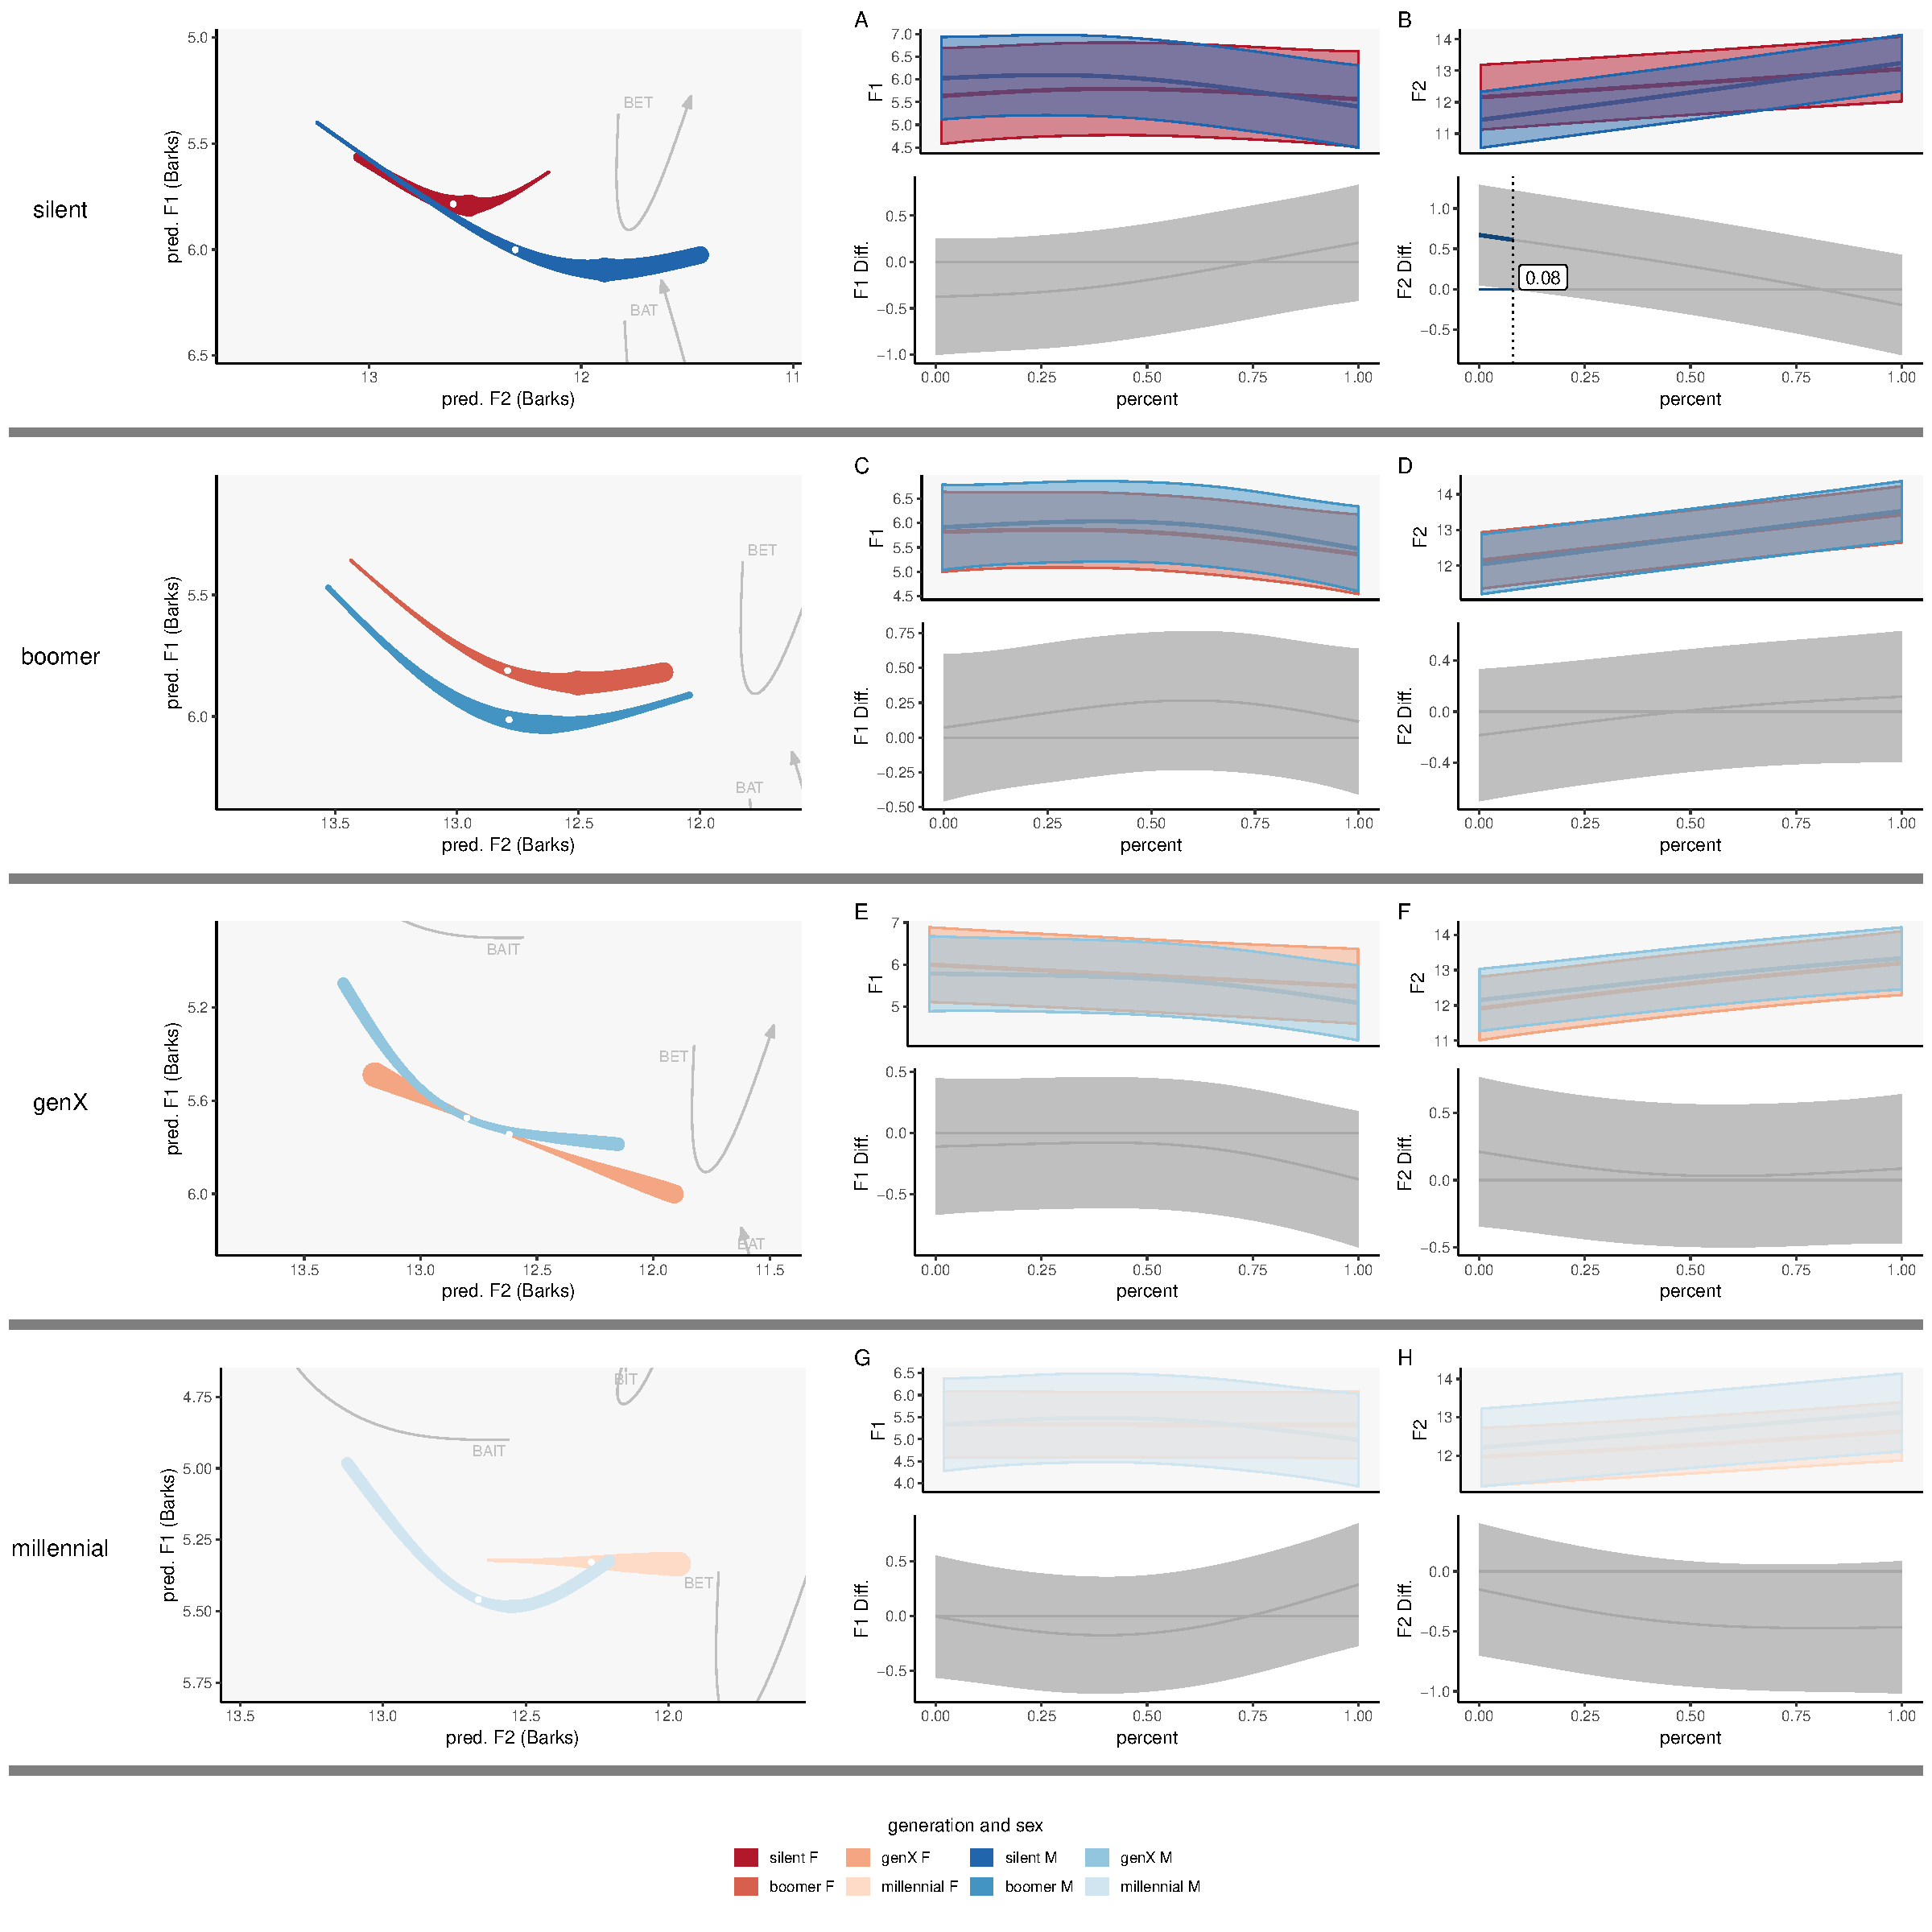
\includegraphics[width=\textwidth]{Figures/BANG/BANG_sex_panel_plot.pdf}
    \caption{Difference smooths comparing the sexes for \bang.}
    \label{fig:bang_diff_smooths_sex_gen}
\end{figure}


\begin{figure}[p]
    \centering
    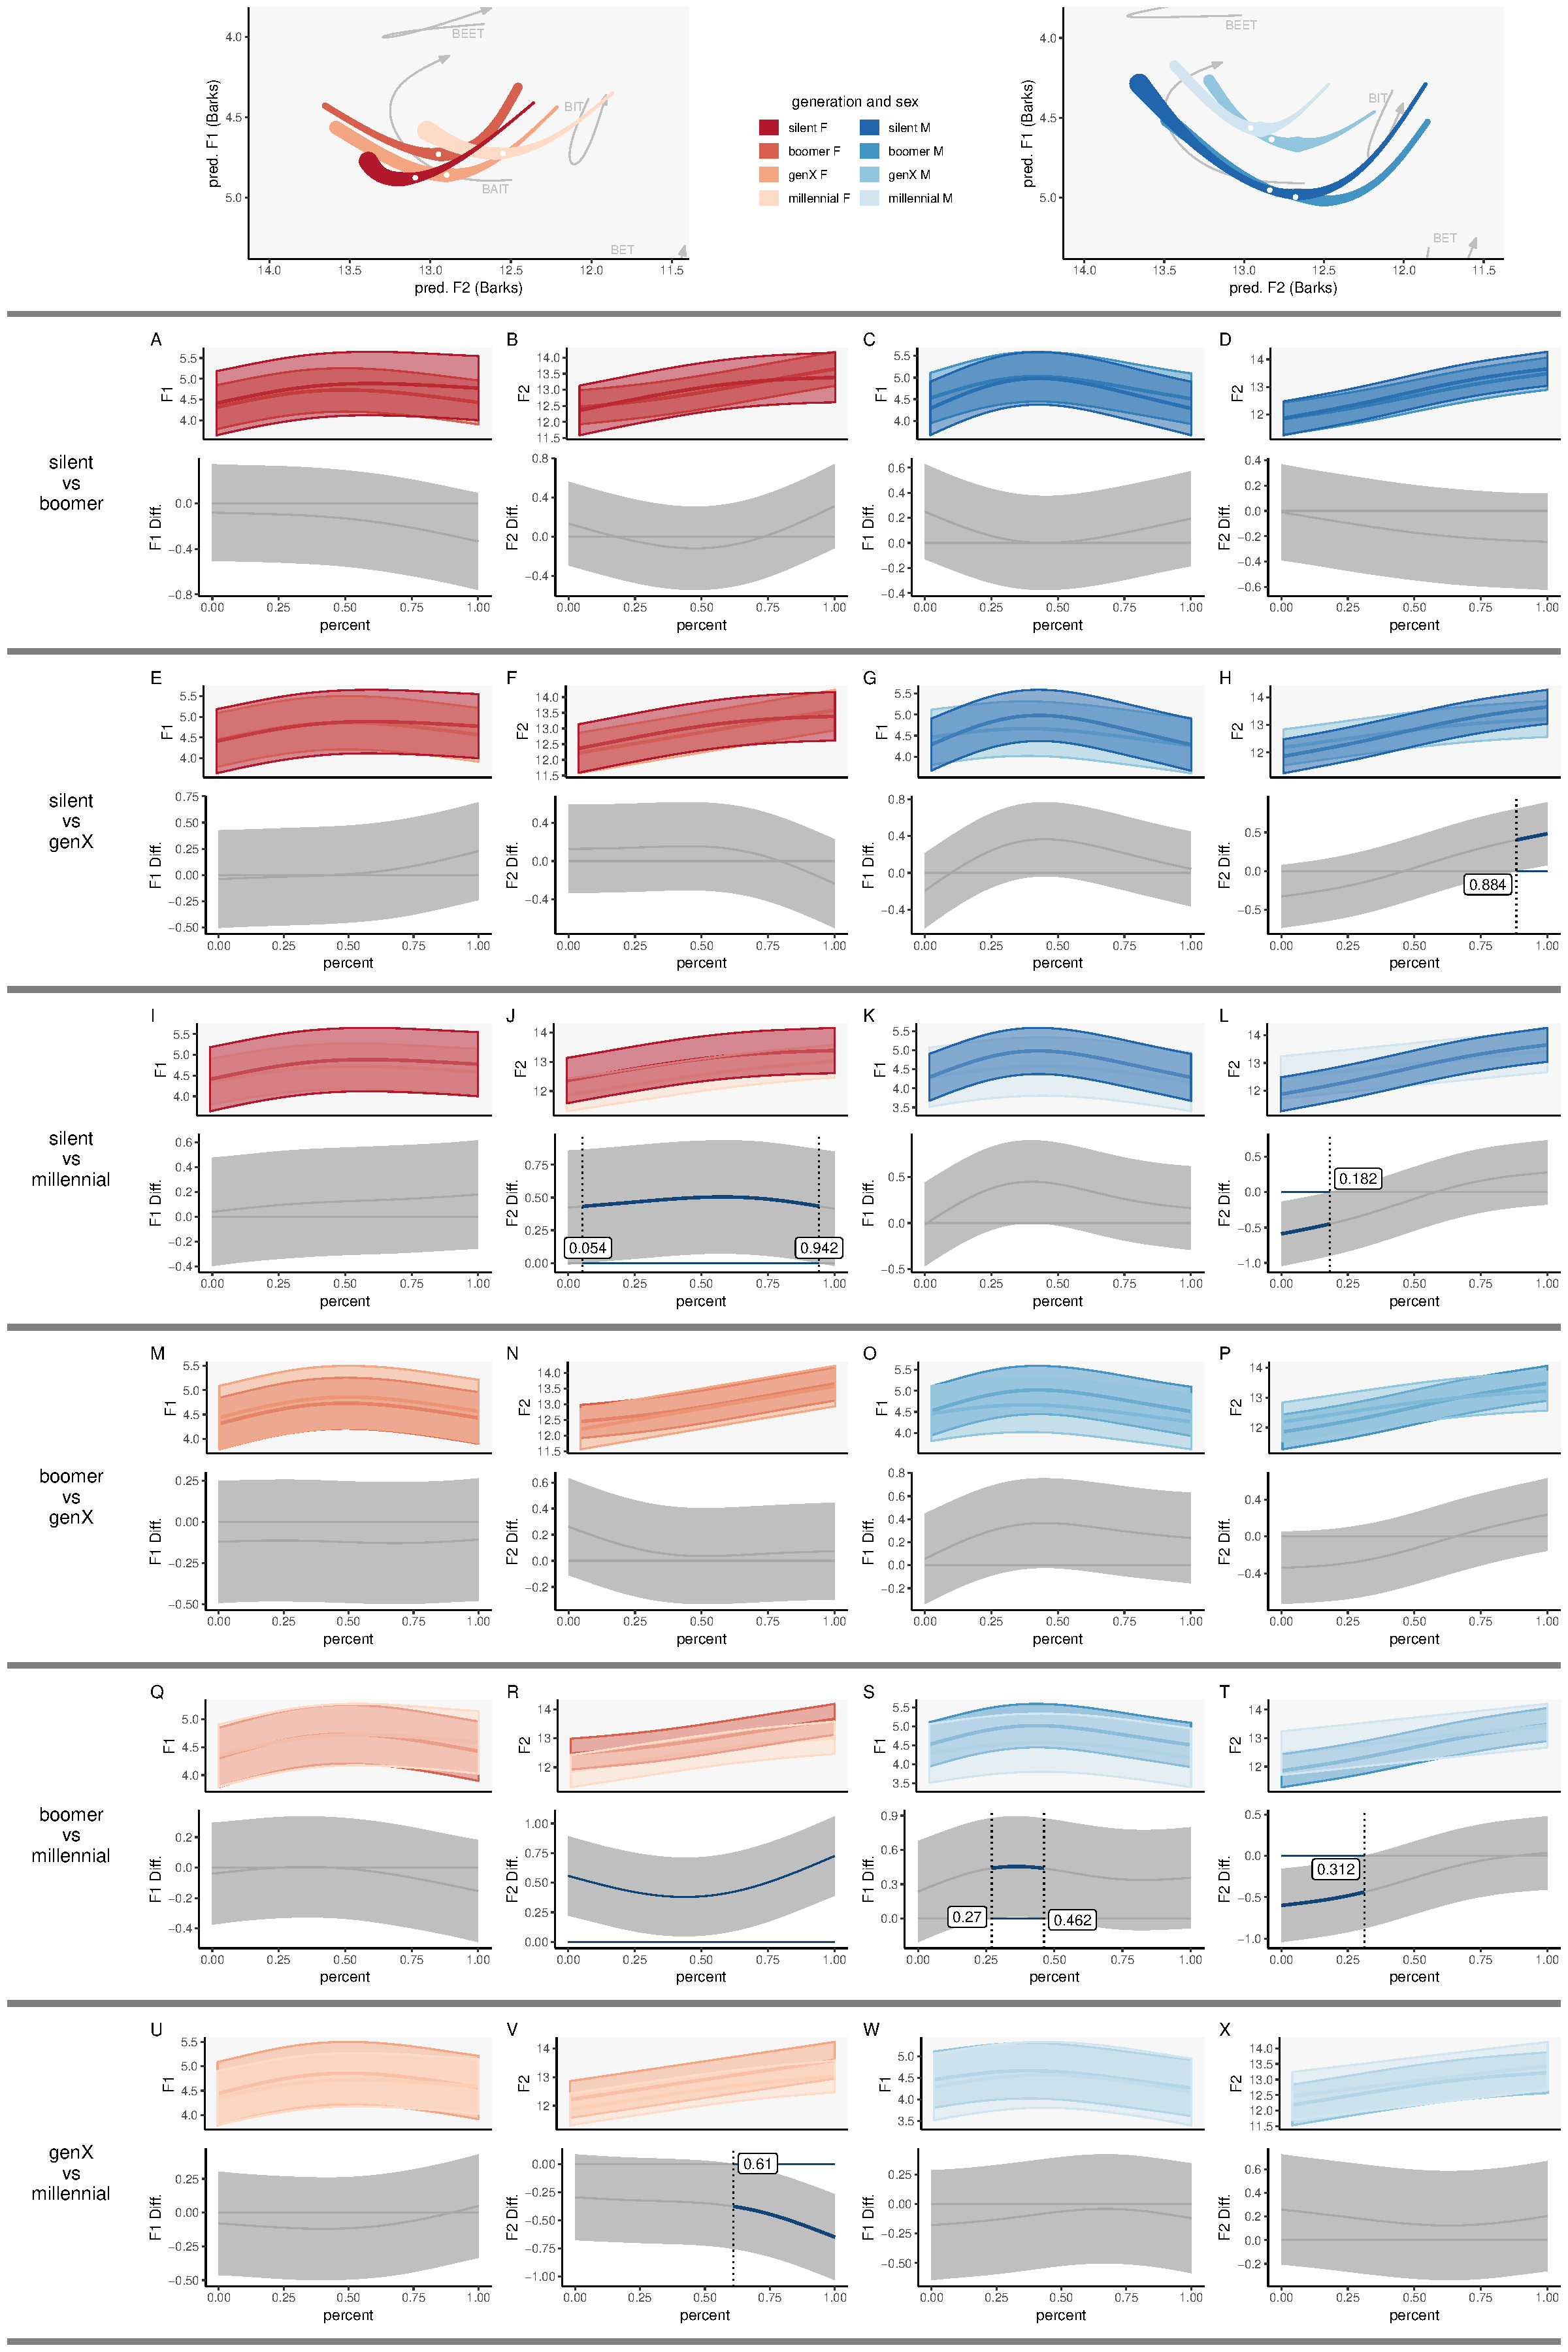
\includegraphics[width=\textwidth]{Figures/BING/BING_detailed_generation_panel_plot.pdf}
    \caption{Difference smooths comparing generation pairs for \bing.}
    \label{fig:bing_diff_smooths_gen}
\end{figure}

\begin{figure}[p]
    \centering
    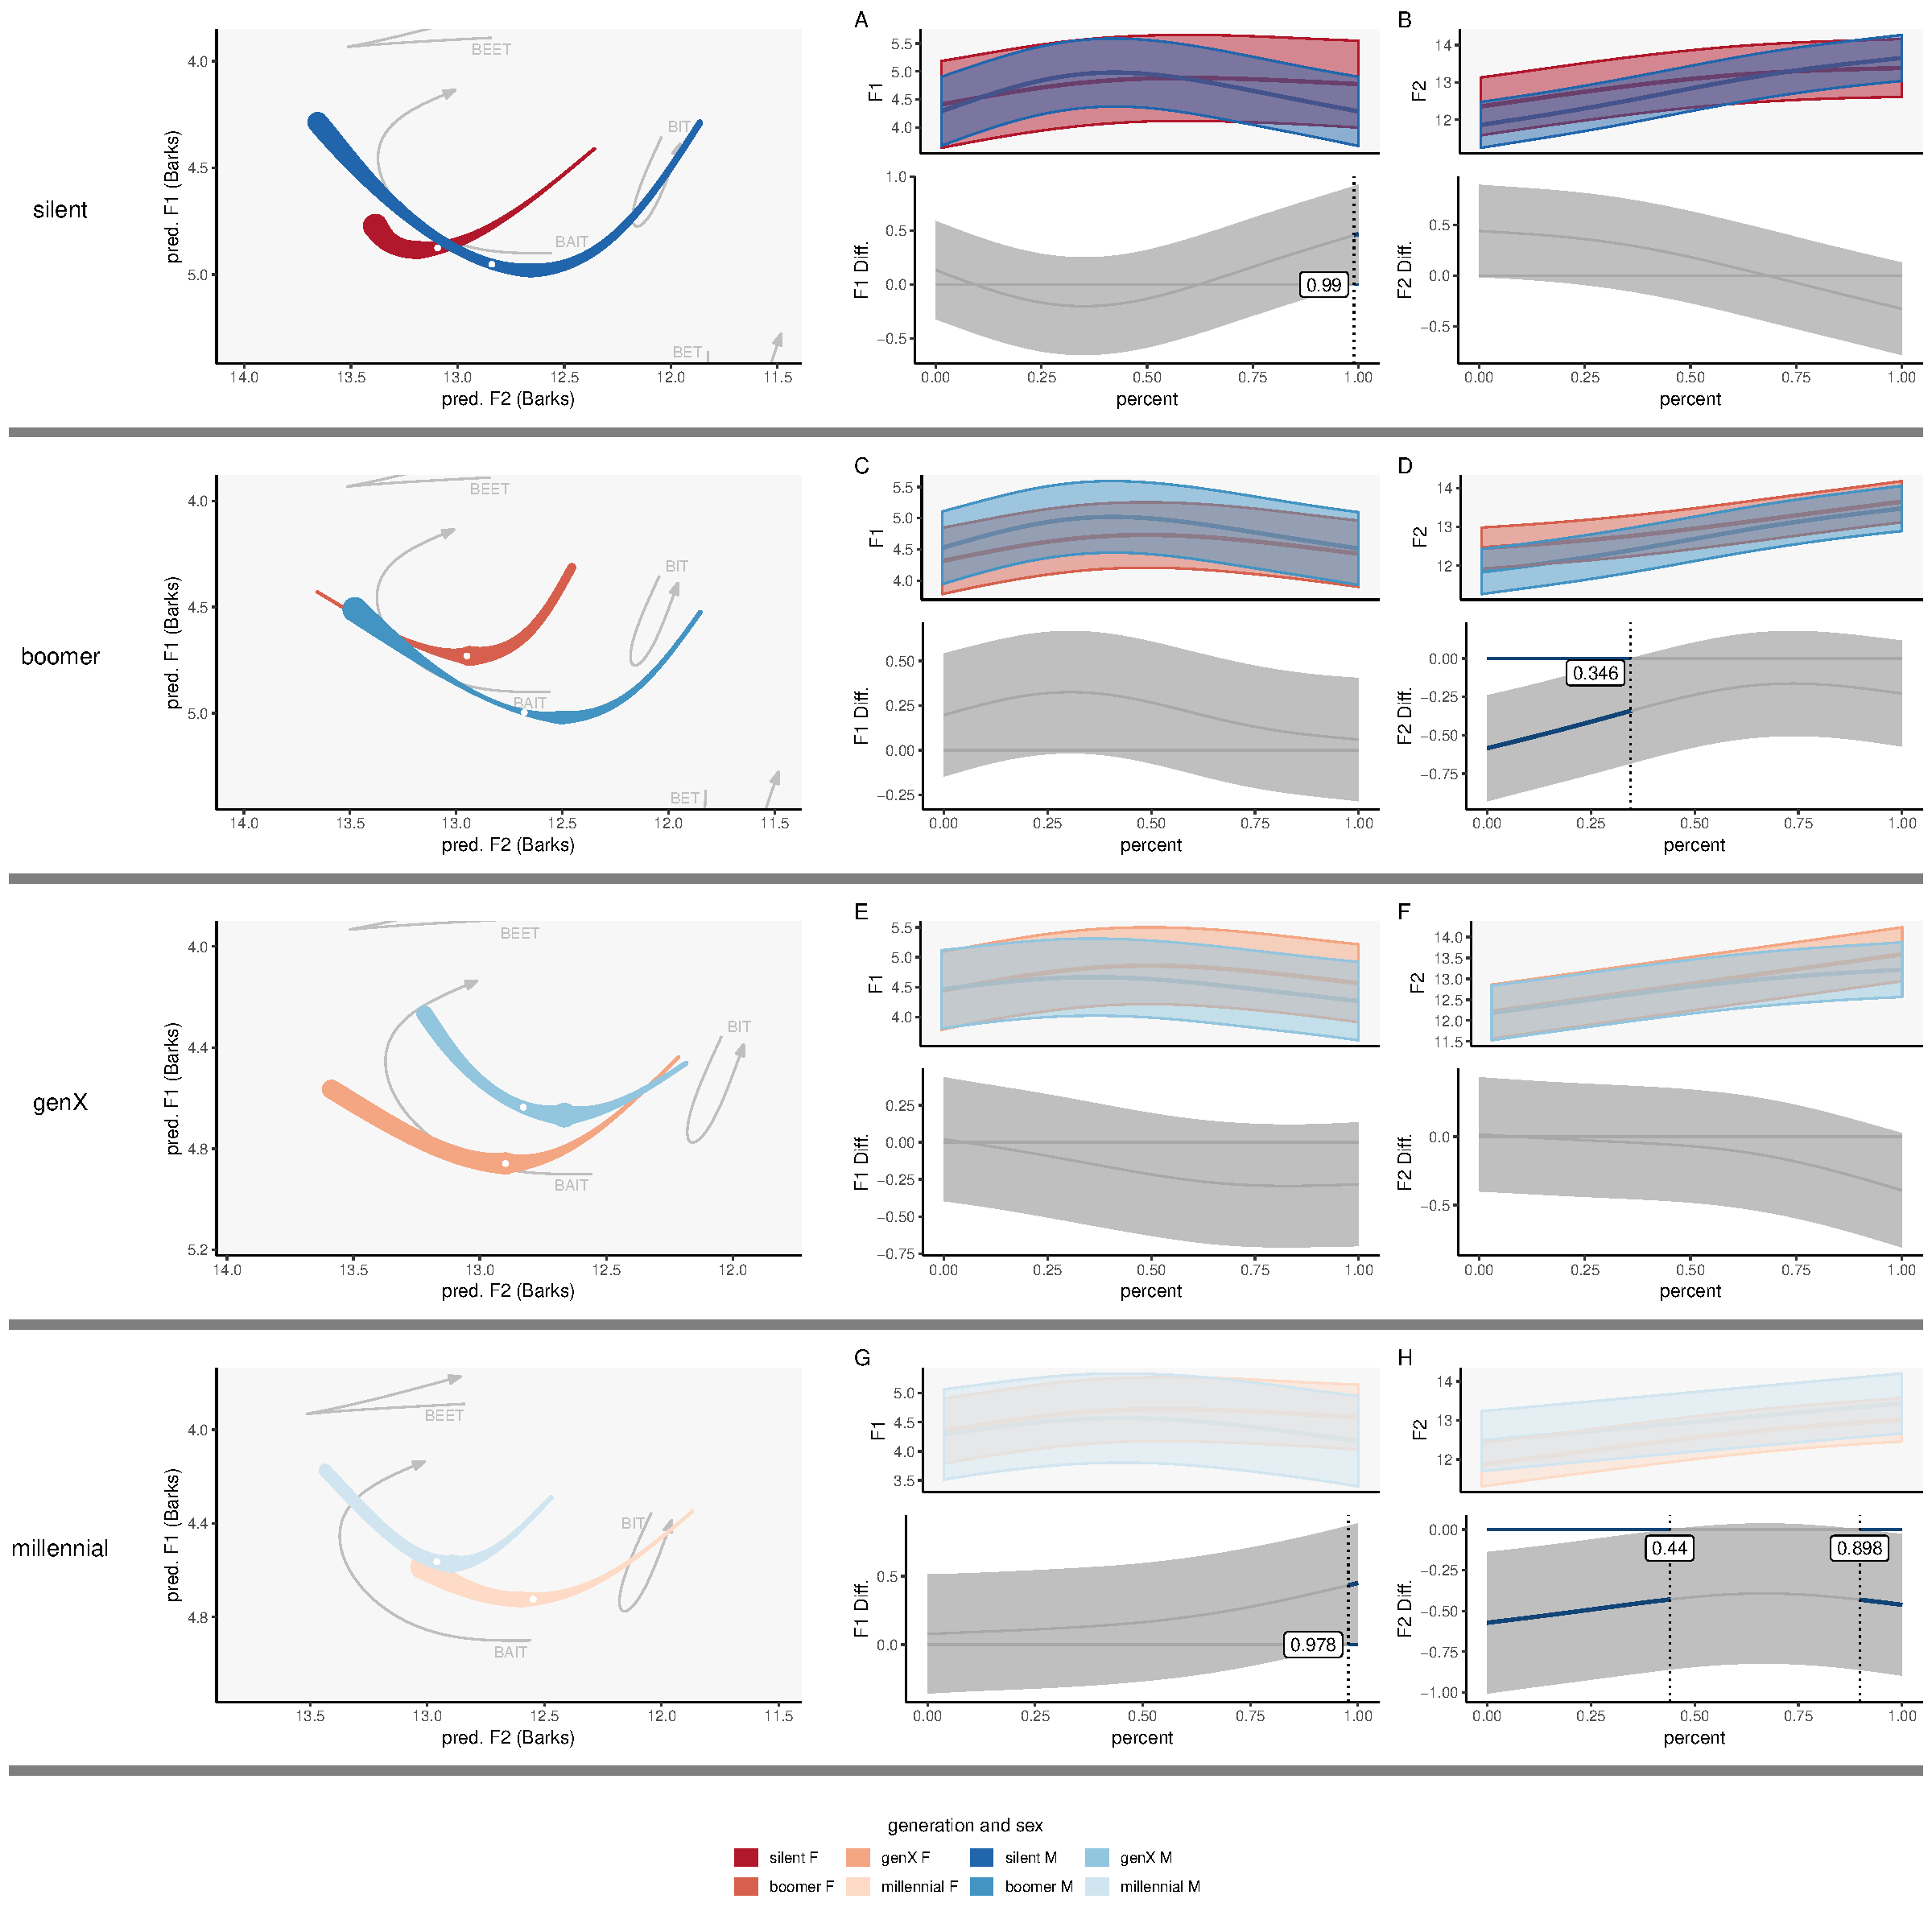
\includegraphics[width=\textwidth]{Figures/BING/BING_sex_panel_plot.pdf}
    \caption{Difference smooths comparing the sexes for \bing.}
    \label{fig:bing_diff_smooths_sex_gen}
\end{figure}




\begin{figure}[p]
    \centering
    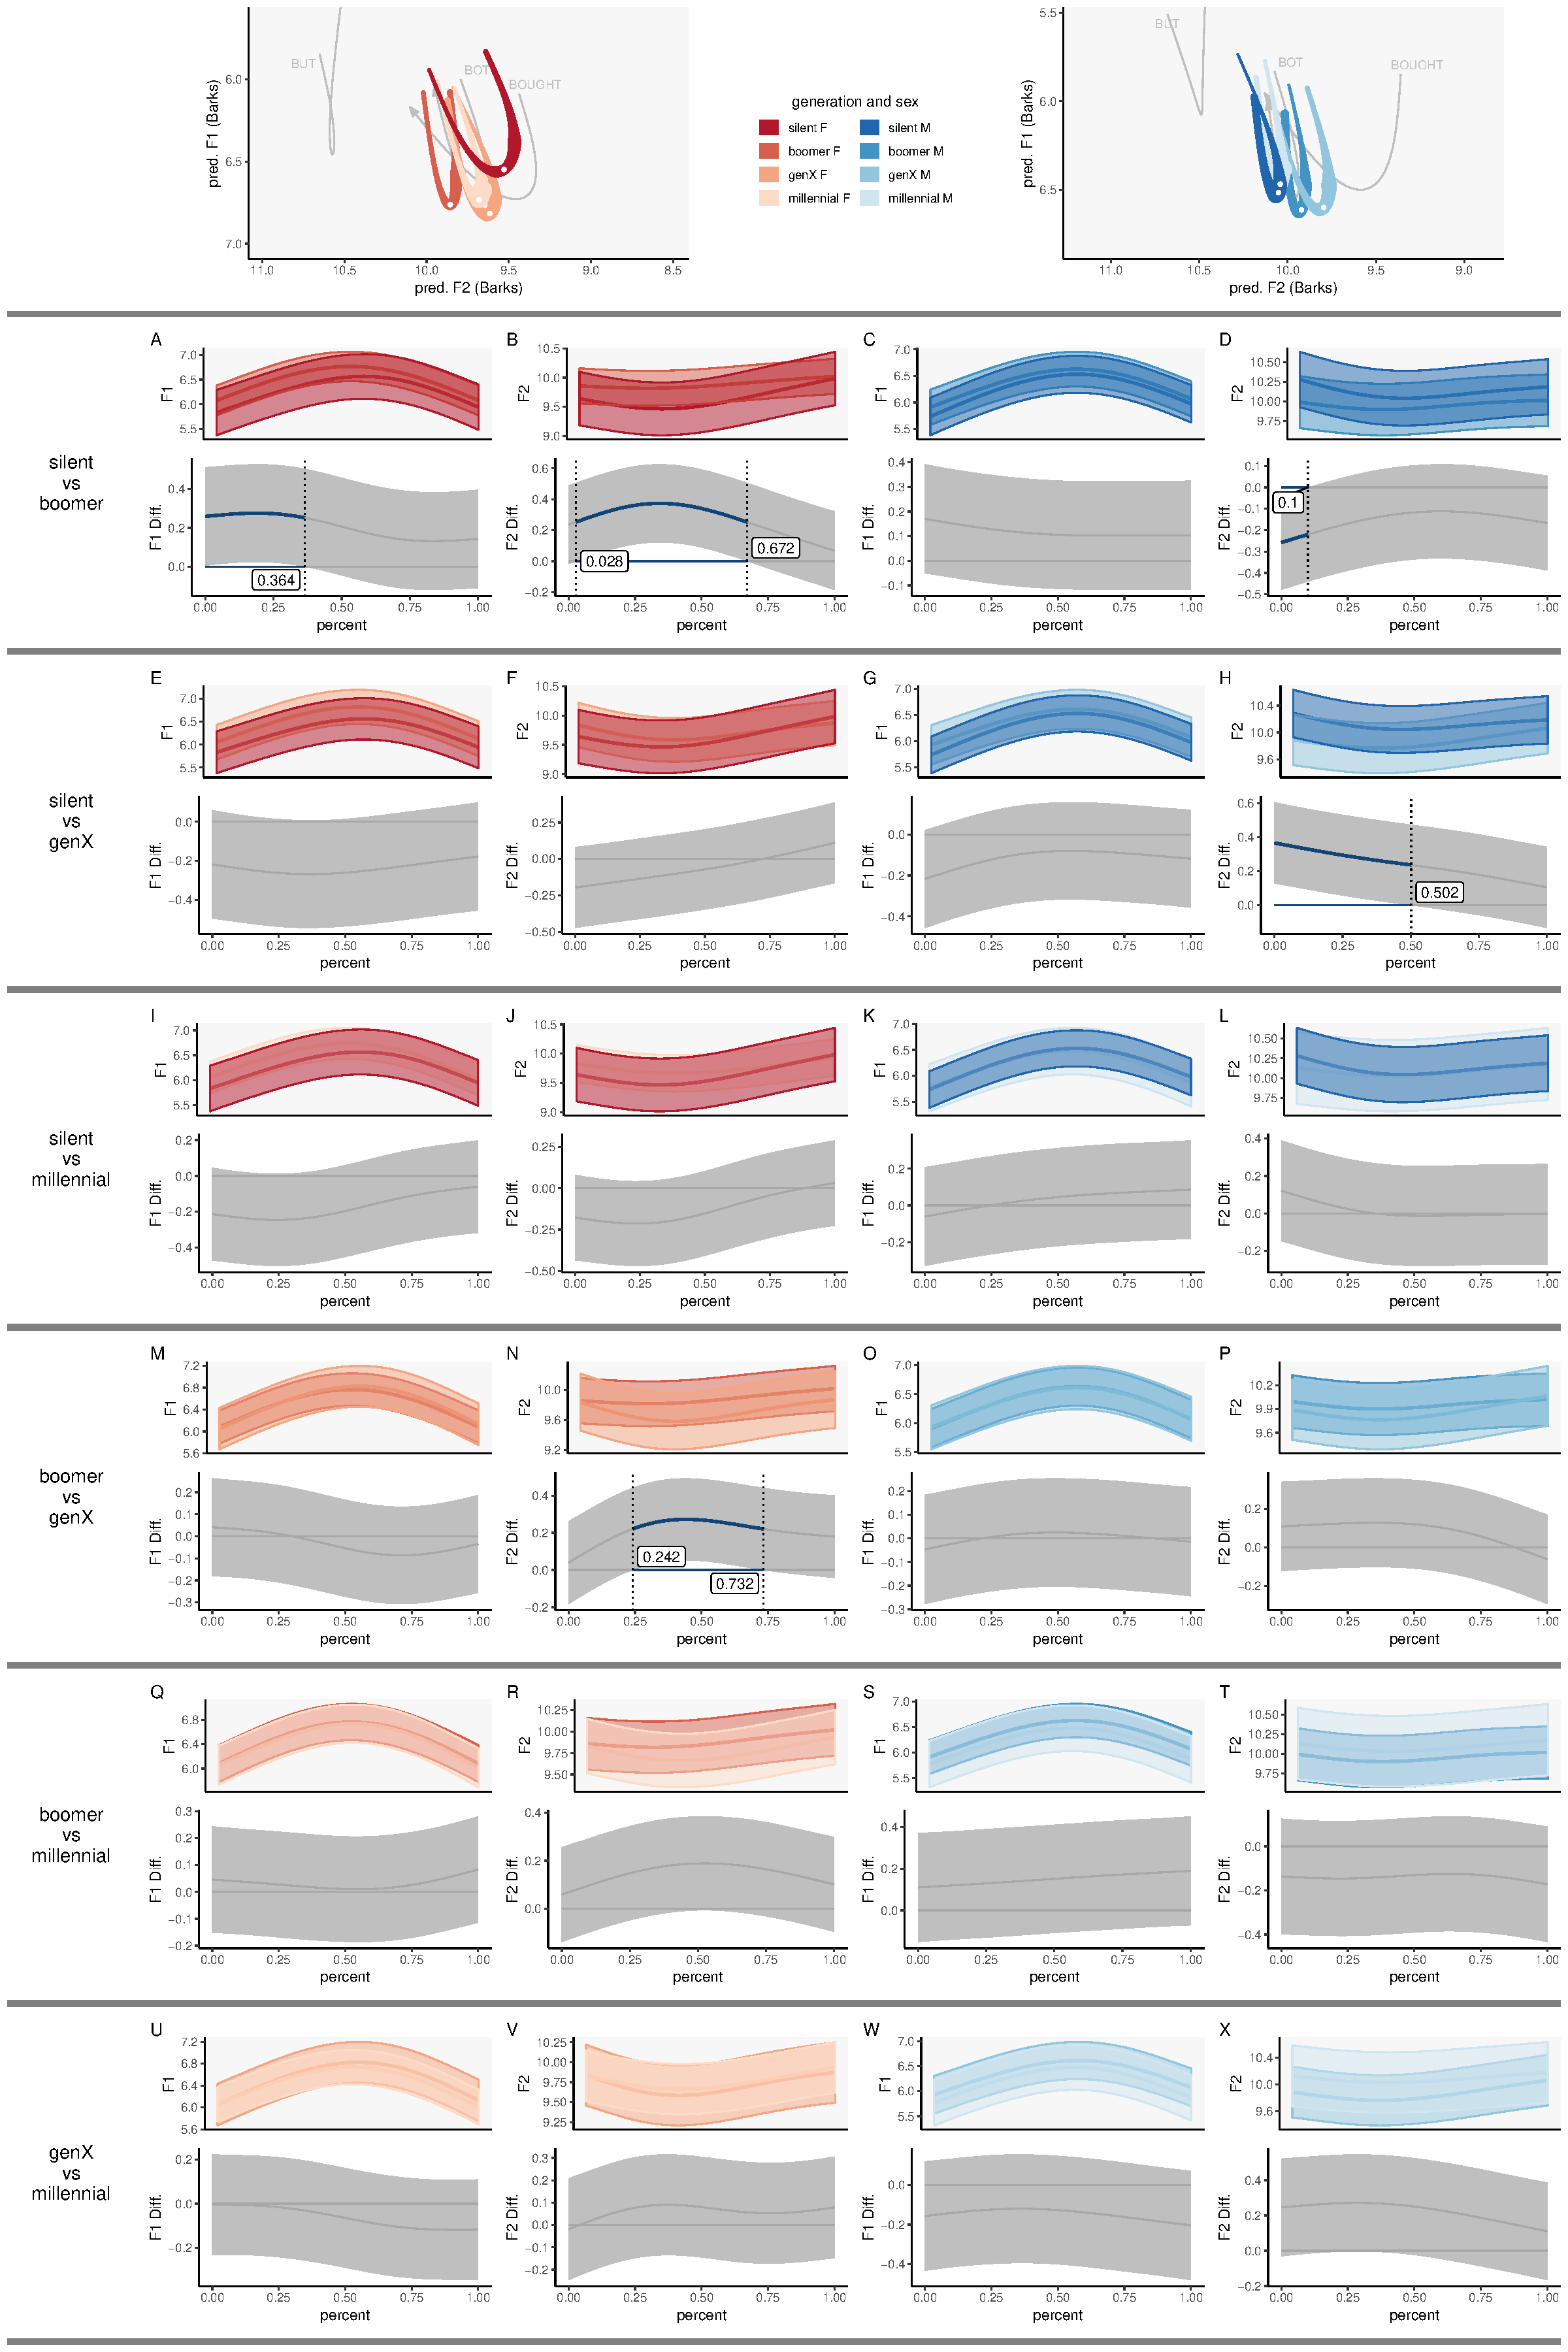
\includegraphics[width=\textwidth]{Figures/BOT/BOT_detailed_generation_panel_plot.pdf}
    \caption{Difference smooths comparing generation pairs for \lot.}
    \label{fig:bot_diff_smooths_gen}
\end{figure}

\begin{figure}[p]
    \centering
    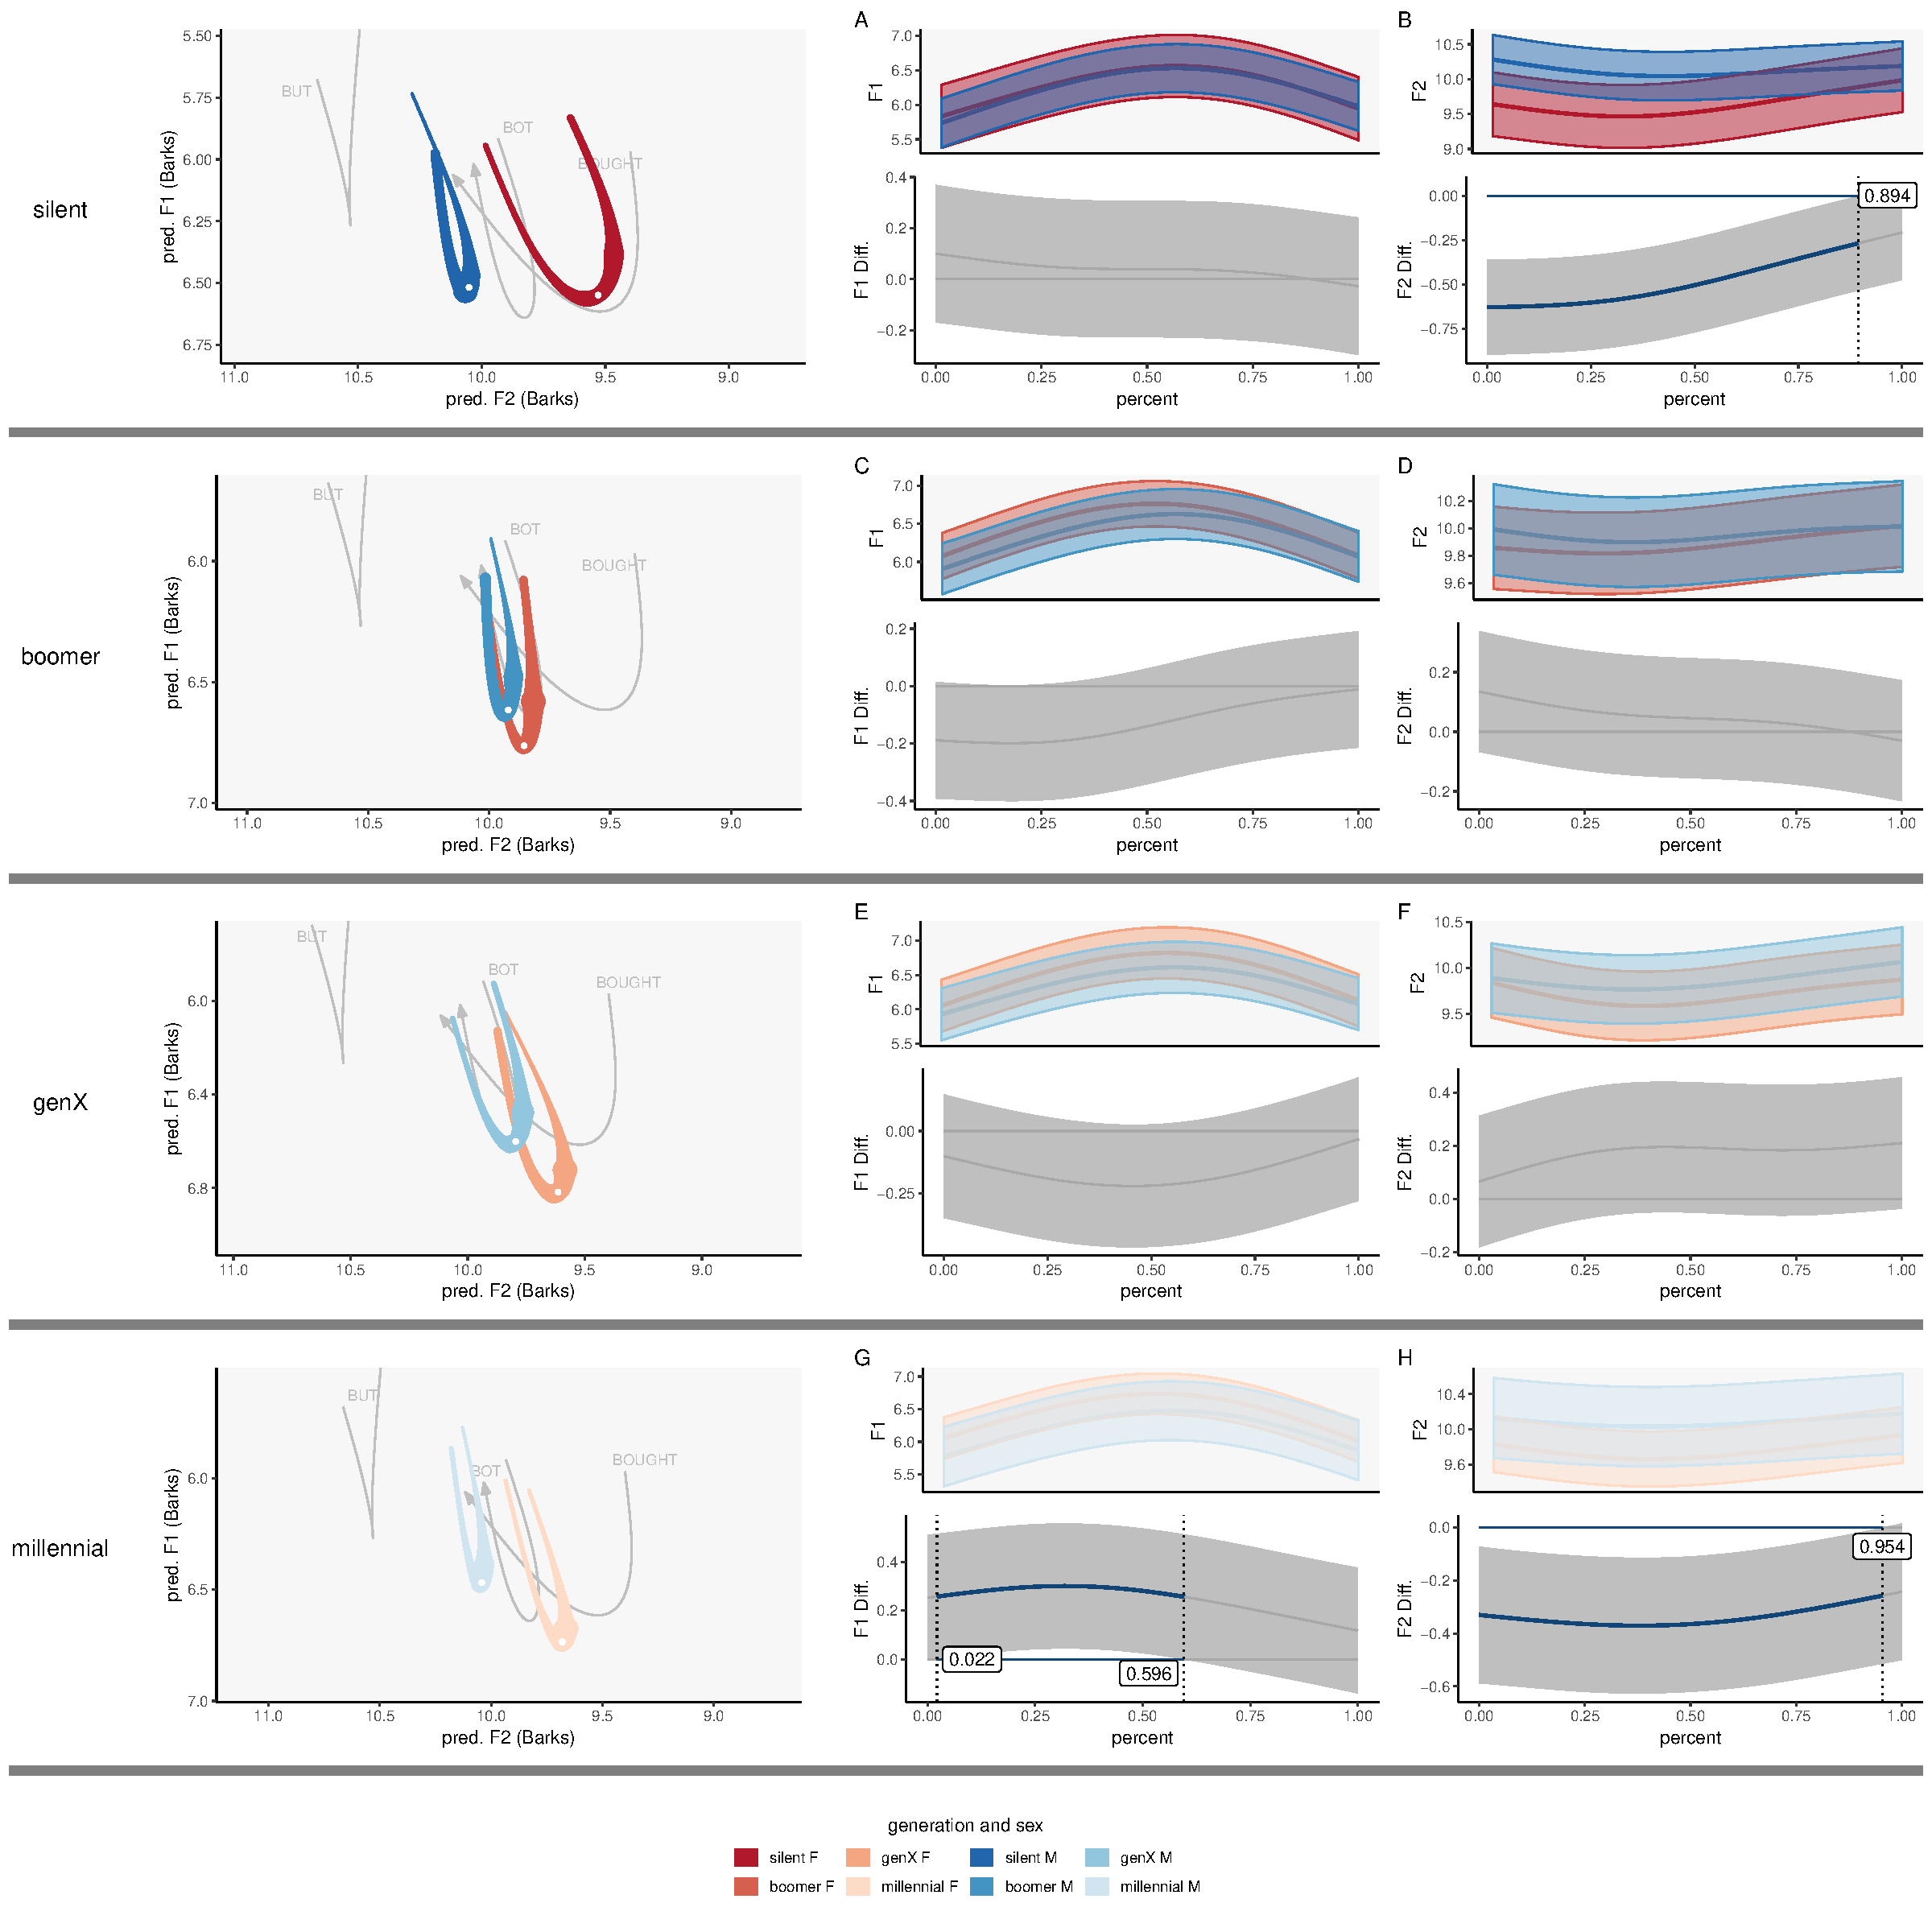
\includegraphics[width=\textwidth]{Figures/BOT/BOT_sex_panel_plot.pdf}
    \caption{Difference smooths comparing the sexes for \lot.}
    \label{fig:bot_diff_smooths_sex_gen}
\end{figure}




\begin{figure}[p]
    \centering
    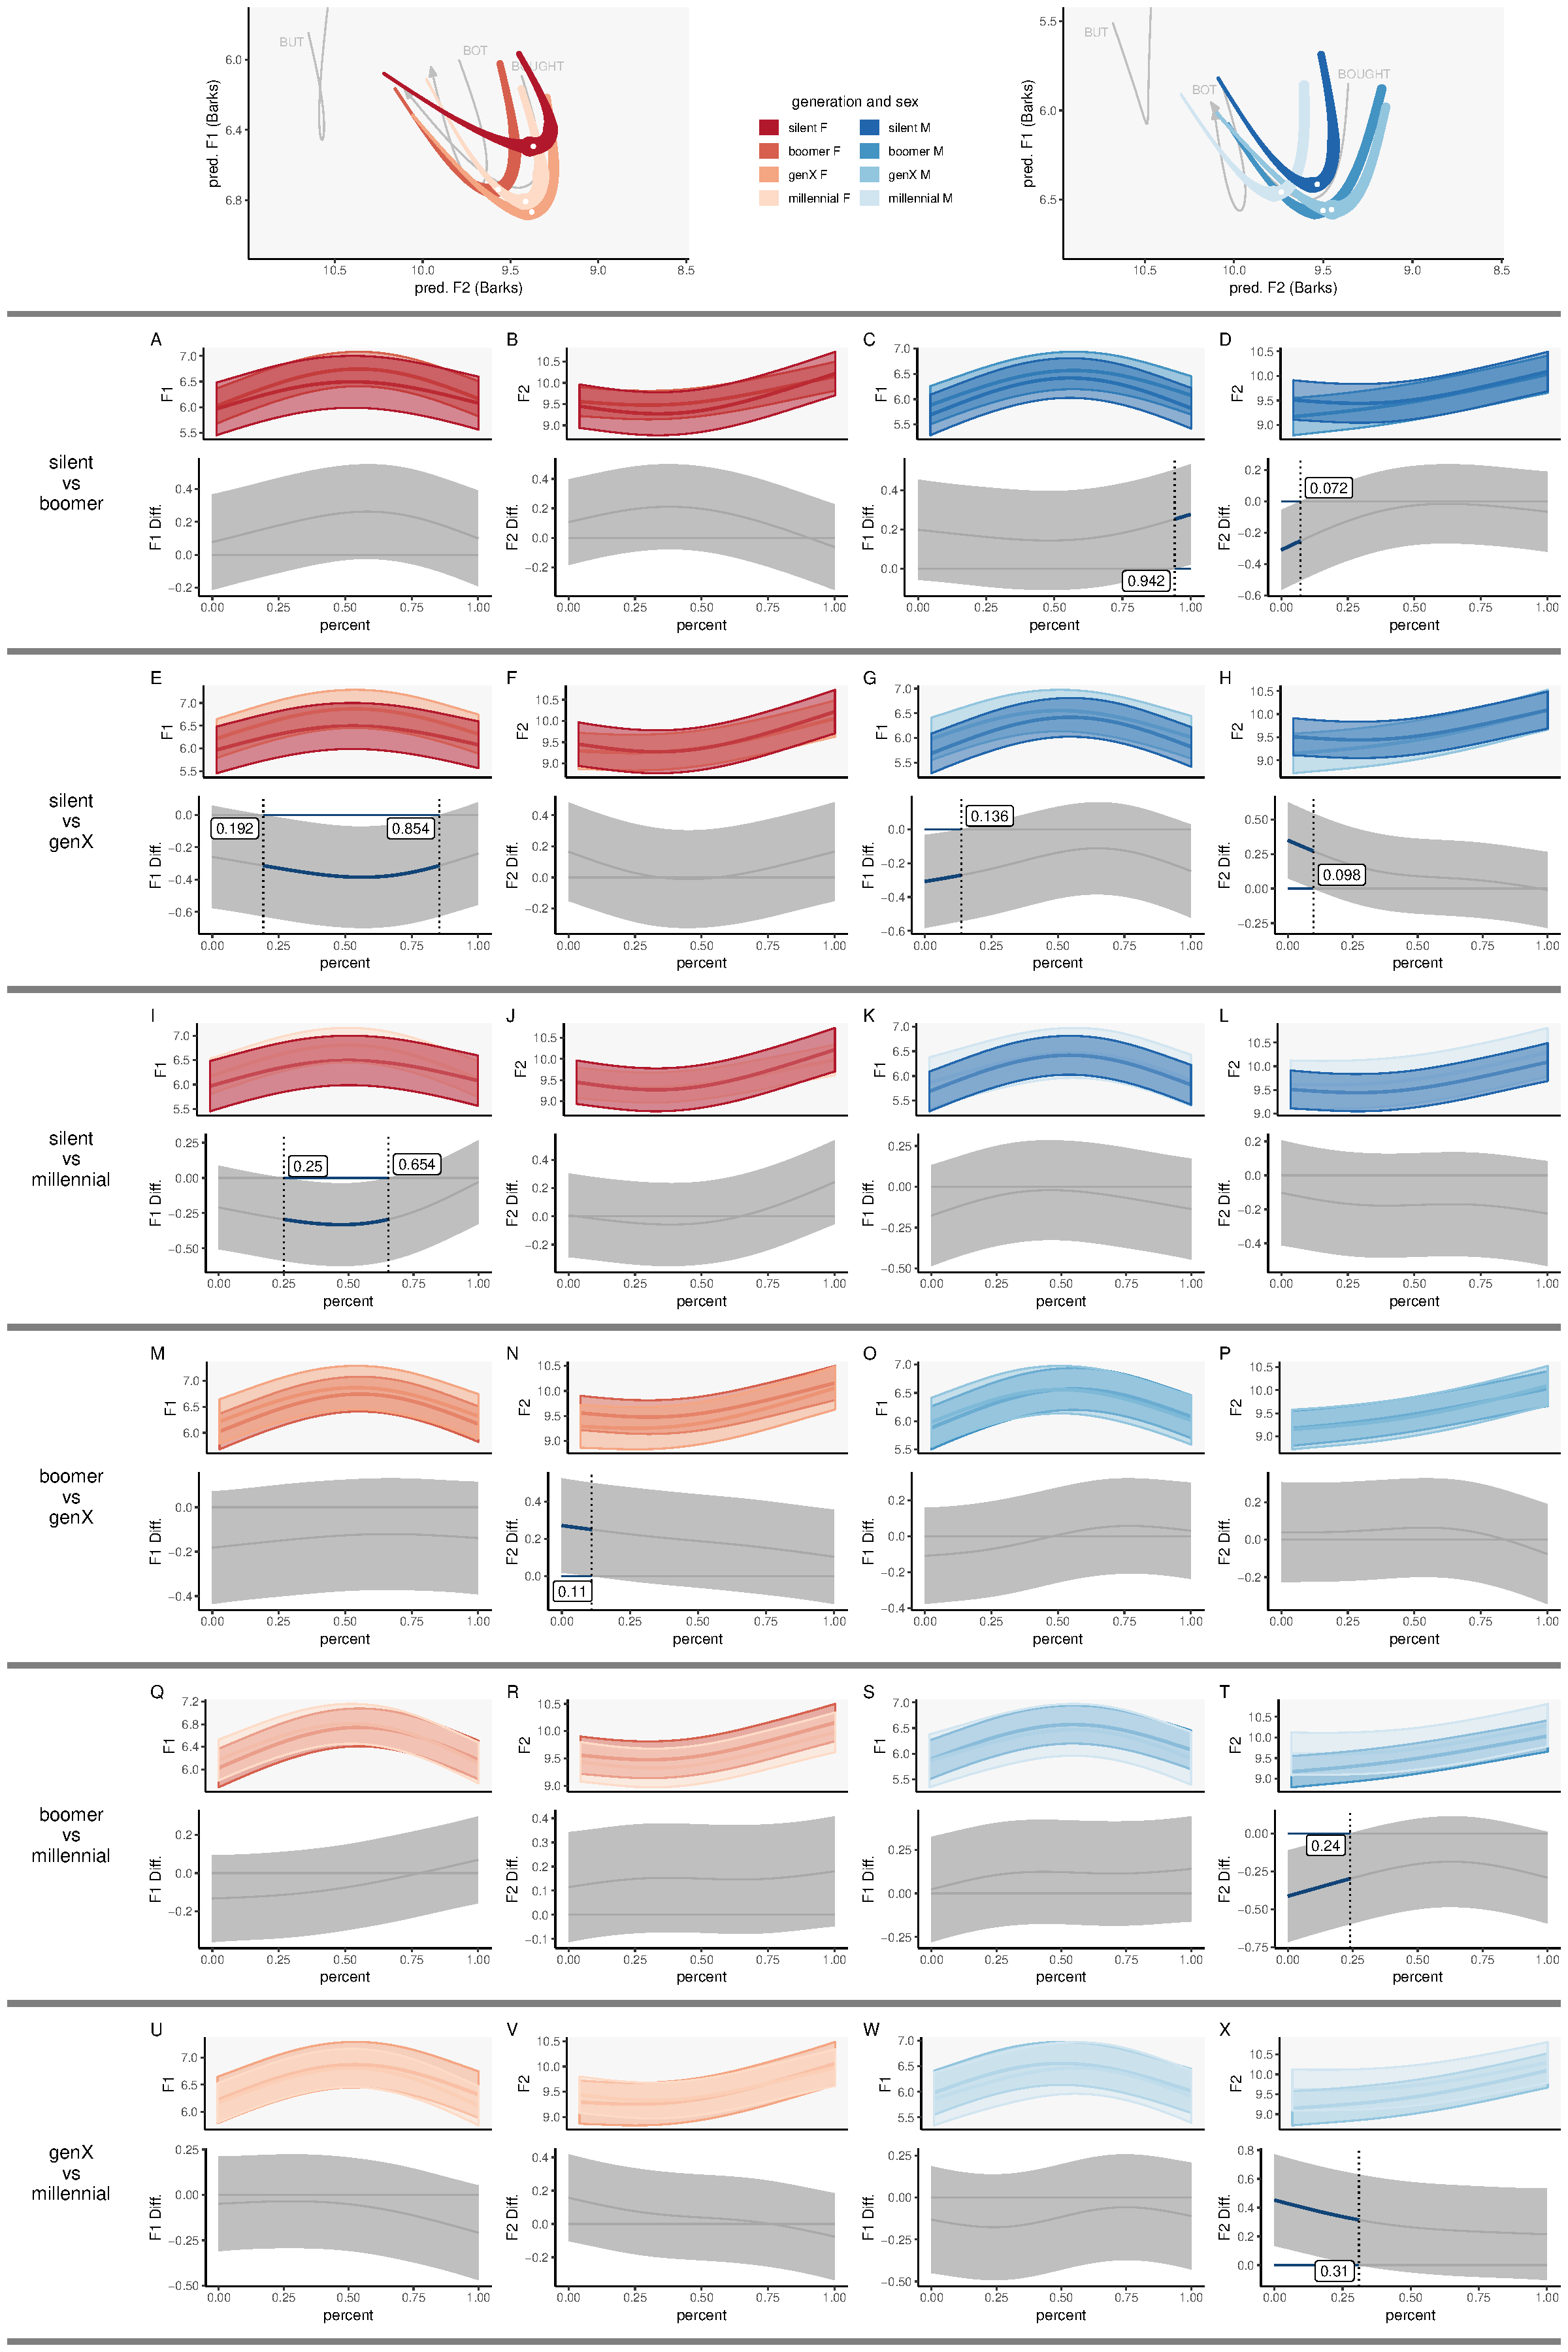
\includegraphics[width=\textwidth]{Figures/BOUGHT/BOUGHT_detailed_generation_panel_plot.pdf}
    \caption{Difference smooths comparing generation pairs for \thought.}
    \label{fig:bought_diff_smooths_gen}
\end{figure}

\begin{figure}[p]
    \centering
    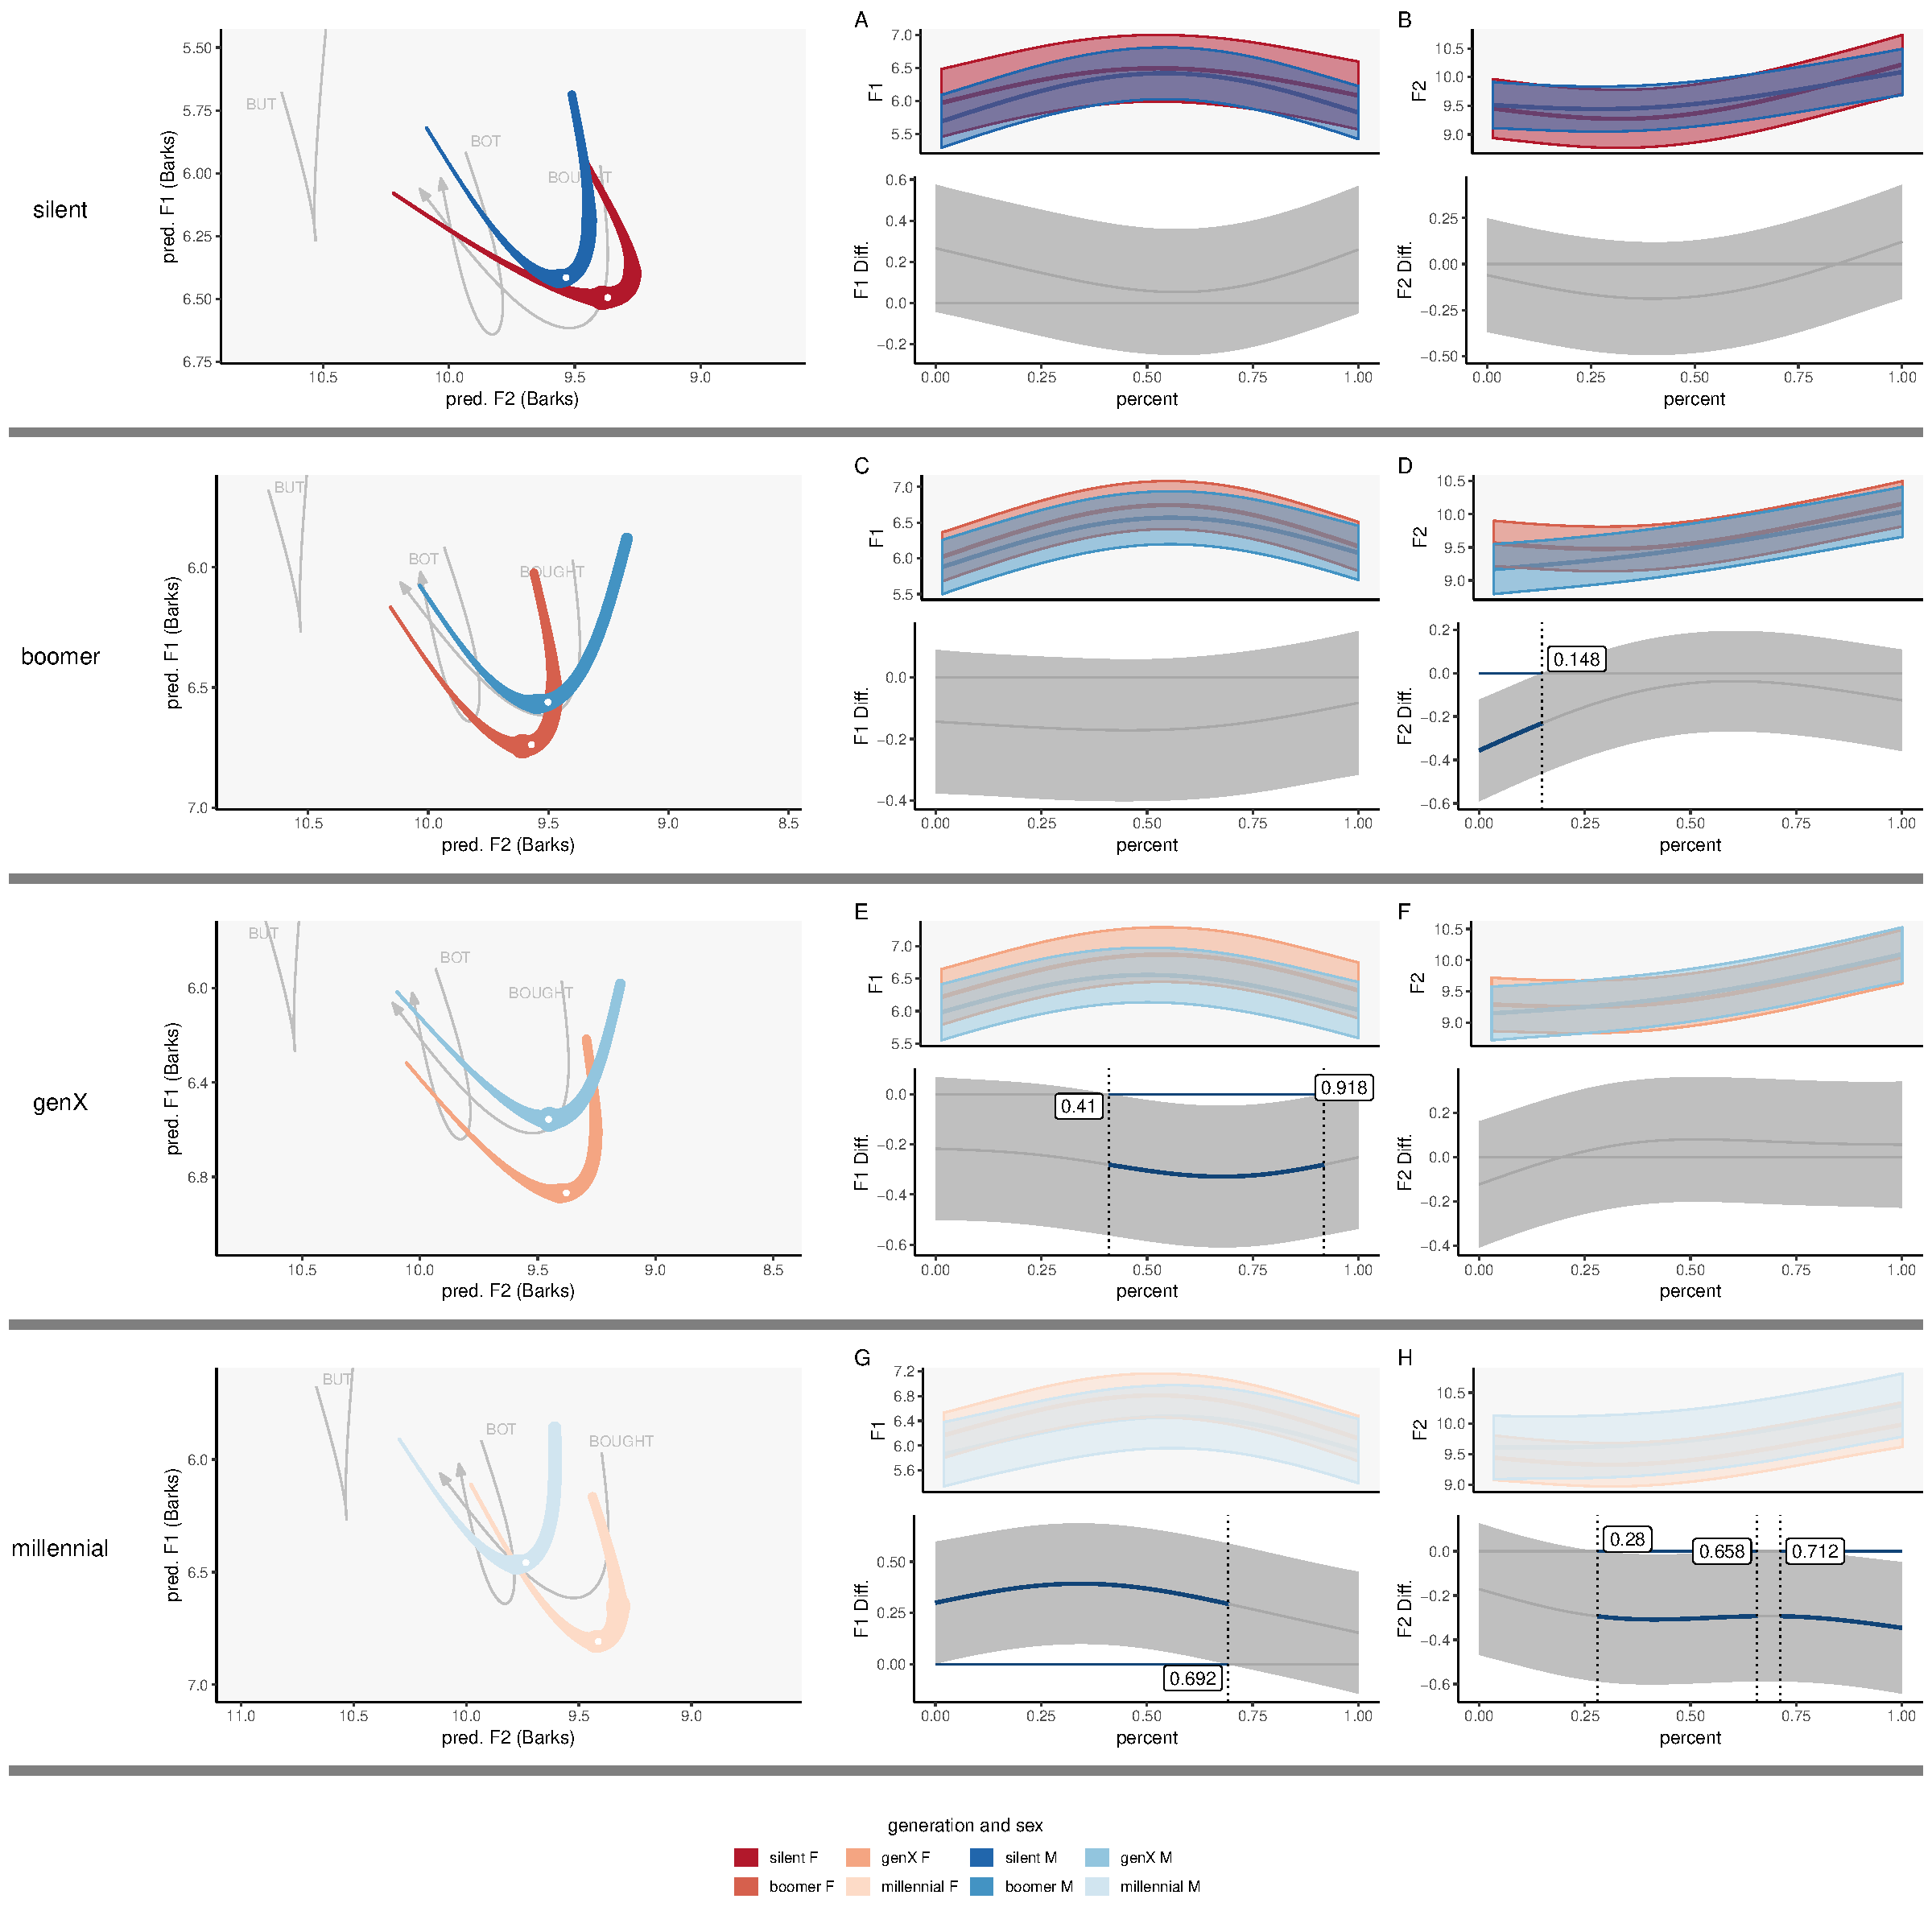
\includegraphics[width=\textwidth]{Figures/BOUGHT/BOUGHT_sex_panel_plot.pdf}
    \caption{Difference smooths comparing the sexes for \thought.}
    \label{fig:bought_diff_smooths_sex_gen}
\end{figure}
